\documentclass[conference,a4paper]{../../IEEEtran}

% *** GRAPHICS RELATED PACKAGES ***
\ifCLASSINFOpdf
  \usepackage[pdftex]{graphicx}
  \usepackage{epstopdf}
  % declare the path(s) where your graphic files are
  % \graphicspath{{../pdf/}{../jpeg/}}
  % and their extensions so you won't have to specify these with
  % every instance of \includegraphics
  % \DeclareGraphicsExtensions{.pdf,.jpeg,.png}
\else
  % or other class option (dvipsone, dvipdf, if not using dvips). graphicx
  % will default to the driver specified in the system graphics.cfg if no
  % driver is specified.
  \usepackage[dvips]{graphicx}
  % declare the path(s) where your graphic files are
  % \graphicspath{{../eps/}}
  % and their extensions so you won't have to specify these with
  % every instance of \includegraphics
  % \DeclareGraphicsExtensions{.eps}
\fi


% *** MATH PACKAGES ***
\usepackage[cmex10]{amsmath}


% *** PDF, URL AND HYPERLINK PACKAGES ***
\usepackage{url}
\usepackage{caption}
\usepackage{subcaption}
\usepackage{morefloats}


% *** Do not adjust lengths that control margins, column widths, etc. ***
% *** Do not use packages that alter fonts (such as pslatex).         ***
% There should be no need to do such things with IEEEtran.cls V1.6 and later.
% (Unless specifically asked to do so by the journal or conference you plan
% to submit to, of course. )


% correct bad hyphenation here
\hyphenation{op-tical net-works semi-conduc-tor}


\begin{document}
%
% paper title
% can use linebreaks \\ within to get better formatting as desired
\title{OMNeT++ Network Simulation}


% author names and affiliations
% use a multiple column layout for up to three different
% affiliations
\author{
\IEEEauthorblockN{Zhen-Huan Hwang and Hasan Mahmood Aminul Islam}
\IEEEauthorblockA{Aalto University, Espoo, Finland\\
zhen-huan.hwang and hasan.islam @aalto.fi}}


% make the title area
\maketitle


\begin{abstract}

OMNeT++ is an open-source network simulation tool and is free for academic usage.
The main objective of this assignment is to familiarise ourselves with OMNeT++.
In this assignment, we use OMNeT++ simulation tool to evaluate three TCP congestion control algorithms under different network characteristics.
We modify host specific TCP parameters to select different TCP congestion control algorithms.
Variation of network characteristics is done through relevant configuration files.
Finally, we provide an analysis of the trace we obtained from OMNeT++ simulation.

\end{abstract}
% IEEEtran.cls defaults to using nonbold math in the Abstract.
% This preserves the distinction between vectors and scalars. However,
% if the conference you are submitting to favors bold math in the abstract,
% then you can use LaTeX's standard command \boldmath at the very start
% of the abstract to achieve this. Many IEEE journals/conferences frown on
% math in the abstract anyway.

% no keywords



\section{Introduction}
% no \IEEEPARstart

OMNeT++ is an open-source network simulation tool and is free for academic usage.
It is accompanied by a rich set of documentation, addons, and examples.
It is therefore a good idea for us in computer networking related fields to familiarise ourselves with OMNeT++.
In order to fulfil this main objective, we will set up a simplified version of Finland national backbone and do some experiments.
This required us to develop the OMNeT++ model, devise and deploy a subnet scheme, configure some routing mechnism to make the model a connected network, and finally deploy TCP test applications in the network.

\subsection{TCP and congestion control}

TCP \cite{tcp} is a connection-oriented, reliable standard transport protocol. TCP is able to recover data that is damaged, lost, duplicated, or delivered out of order through Internet. TCP sender uses sequence numbers and acknowledgements from a receiver to recover for flow control and error control.

TCP provides flow and congestion control mechanisms through the use of congestion window. TCP starts a retransmission timer when an downstream segment is passed down to IP. If there is no acknowledgement from the receiver for the data in a given segment before the timer expires, then the segment is retransmitted. If the network is congested, the sender increases the window size by a fixed number every RTT. In response to congestion detection, the sender decreases the transmission rate by a multiplicative factor, for instance, the congestion window is decreased by half. This algorithm is known as Additive increase, multiplicative decrease (AIMD) of the sending rate. The acknowledgement (ACK) number from receiver determines a range of acceptable sequence numbers beyond the last segment successfully received. 


TCP Reno is a variant of basic TCP congestion protocol. It applies four congestion control mechanisms: slow-start, congestion avoidance, fast retransmit and fast recovery. Slow-start and congestion avoidance algorithms are utilized to control the amount of outstanding data being pushed into the network. TCP sender uses congestion window to limit the amount of data in sender side to be injected into the network before receiving an acknowledgement (ACK). Flow control is achieved through receiver's advertised window (\texttt{rwnd}) on the amount of outstanding data. Another state variable, the slow start threshold (\texttt{ssthresh}), defines the margin to promote the sender switching from the slow-start to congestion avoidance algorithm.

At the beginning of transmission into a network with unknown conditions, TCP applies slow-start algorithm to determine the available capacity of the network instead of injecting large burst of data congesting the network. This algorithm is also used after loss recovery by the retransmission timer. A non standard, experimental TCP extension states that the initial value of \texttt{cwnd} can be defined as the following equation \cite{RFC2414}:

\begin{equation}
   cwnd = min (4\times SMSS, max (2 \times SMSS, 4380 bytes))
  \label{eqn1}
\end{equation}

where sender maximum segment size (SMSS) is the size of the largest segment that the sender can transmit. This value can be based on the maximum transmission unit of the network, largest segment the receiver is willing to accept or other factors. The initial value of \texttt{ssthresh} is set arbitrarily high and reduced upon congestion detection. 



Congestion avoidance algorithm allows the sender to increase the \texttt{cwnd} by SMSS per RTT. The value of \texttt{ssthresh} is adjusted while detecting segment loss using retransmission timer and the given segment has not yet been resent by way of the retransmission timer, the value is set by Equation~\ref{eqnn}.

\begin{equation}
  ssthresh = max (FlightSize  / 2, 2 \times SMSS)
  \label{eqnn}
\end{equation}

where, \texttt{FlightSize} is the amount of outstanding data in the network. 


When TCP receiver detects arrival of an out of order segment, it immediately sends duplicate ACK to TCP sender that includes the expected sequence number. This ACK is a duplicate of an ACK which was sent previously. From the sender's point of view, a duplicate ACK can be caused by a lost segment or just a reordering of segments. When incoming data segments fill in all or part of a gap in the sequence space, TCP receiver immediately sends an ACK.


Fast Retransmit algorithm is used to detect and repair losses based on incoming duplicate ACKs. Fast Retransmit and Fast Recovery of TCP Reno is used together. The arrival of 3 duplicate ACKs determine the lost of a segment and TCP starts retransmitting a missing segment without waiting for the retransmission timer. The \texttt{cwnd} is set to \texttt{ssthresh} plus 3*SMSS. Therefore, Fast Recovery takes place to promote the transmission of new data until a non-duplicate ACK arrives. 

Generally, TCP Reno \cite{tcpreno} is not able to recover multiple losses of packets in a single flight. In TCP Reno, Fast Recovery exits upon the reception of new ACK. TCP NewReno is the modification of the standard implementation of the Fast Retransmit and Fast Recovery algorithms. The modification introduces partial acknowledgements and a new variable \texttt{recover}. Acknowledgement for a retransmitted packet will acknowledge some but not all of outstanding packets being transmitted. It is known as partial acknowledgement. The value of \texttt{recover} records the highest sequence number transmitted. When a TCP sender receives three duplicate ACKs, the value of \texttt{ssthresh} is reduced to half of the current congestion window and the TCP sender enters fast retransmit mechanism to recover the lost segment. When an ACK arrives, TCP New Reno will determine whether it acknowledges all of the data up to and including \texttt{recover}. If it is not affirmative, then the packet acknowledged by partial acknowledgement is retransmitted. This process continues until an acknowledgement, denoting the highest sequence number already transmitted, arrives and thereafter TCP NewReno \cite{tcpnewreno} will leave the fast recovery setting the value of \texttt{cwnd} to \texttt{ssthresh}. Then congestion avoidance algorithm takes place.


TCP Vegas \cite{brakmo1995tcp} is a congestion avoidance algorithm based on packet delay rather than packet loss to control the transmission rate. TCP Vegas detects congestion based on increasing Round-Trip Time (RTT) values of the packets in the connection. The algorithm depends heavily on accurate calculation of the Base RTT value. If it is too small then throughput of the connection will be less than available capacity and the large value may overrun the connection.

\section{Implementation}
We use OMNeT++ as simulation tool. In this assignment, we have performed networking simulation and utilize the INET2 module.

Figure \ref{fig1} illustrates our test environment set up which consists of seven routers running OSPFv2 and five local area networks.
WAN links are optical fibre with 20Mbps bandwidth and 1ms delay.
The LANs are 100Mbps Ethernet computer LANs and 1Gbps Ethernet CDN networks.
All red links have IP addresses in 192.173.0.0/24 subnet and all green links have IP address from 201.162.5.64/27 subnet.
TCP test applications are run in the hosts attached to Turku LAN and to Oulu LAN.
The test applications establish the connection at 6s after the start of the simulation and transfer 64MiB of data from Turku to Oulu. 


\begin{figure}[h]
\begin{center}
\includegraphics[scale=0.5]{plan.eps}
\caption{Test network -- OurSuomi}
\label{fig1}
\end{center}
\end{figure}


\subsection{Challenges}
One major challenge we encountered was that we must hack the INET\footnote{http://inet.omnetpp.org/} framework to get our simulation running.
OSPFv2 implementation for OMNeT++ does not support passive interface which connects a LAN network and does not receive OSPF messages.
In addition, serializer for OSPF messages was missing so Pcap recorder crashes whenever it receives an OSPF message.
We added a stub into IPv4 serializer to make OSPF messages ignored.
The other hack we did to INET framework is due to that the OSPF implementation tries to update routing table for nonexistent interfaces.
We changed the handler so it simply ignores such updates rather than causing a fatal error.

The last chanllenge is the the simulations are CPU intensive and the output files are large.


\section{Experiments}

We shall compare different TCP congestion control algorithms with respect to different network characteristics.
For this we selected three congestion algorithms: TCP Vegas, TCP Reno, and TCP New Reno.
The main reason behind choosing these three algorithms is that Vegas is sensitive to delay, Reno and New Reno are sensitive to packet loss.

We set up 9 different scenarios:
\begin{itemize}
\item Scene 1: TCP Reno + Delay in core network
\item Scene 2: TCP Reno + Packet error in core network
\item Scene 3: TCP Reno + Router failures in core network
\item Scene 4: TCP New Reno + Delay in core network
\item Scene 5: TCP New Reno + Packet error in core network
\item Scene 6: TCP New Reno + Router failures in core network
\item Scene 7: TCP Vegas + Delay in core network
\item Scene 8: TCP Vegas + Packet error in core network
\item Scene 9: TCP Vegas + Router failures in core network
\end{itemize}

For network delay, we tested four different values: 10ms, 50ms, 200ms, and 250ms.
For packet error, we tested four different rates: 1\%, 5\%, 10\%, and 20\%.
The story of router failure is: at 9s, rTampere crashes; at 19s, rTampere restores and rHelsinki crashes; at 25s, rHelsinki restores.
Once rTampere crashes, the route from Turku will be forced to go though rHelsinki if not already.
The crash of rHelsinki that follow will then force a route change through rTampere.


\section{Result}

% ==== delay

\begin{figure}
 \centering
 \begin{subfigure}[b]{0.2\textwidth}
  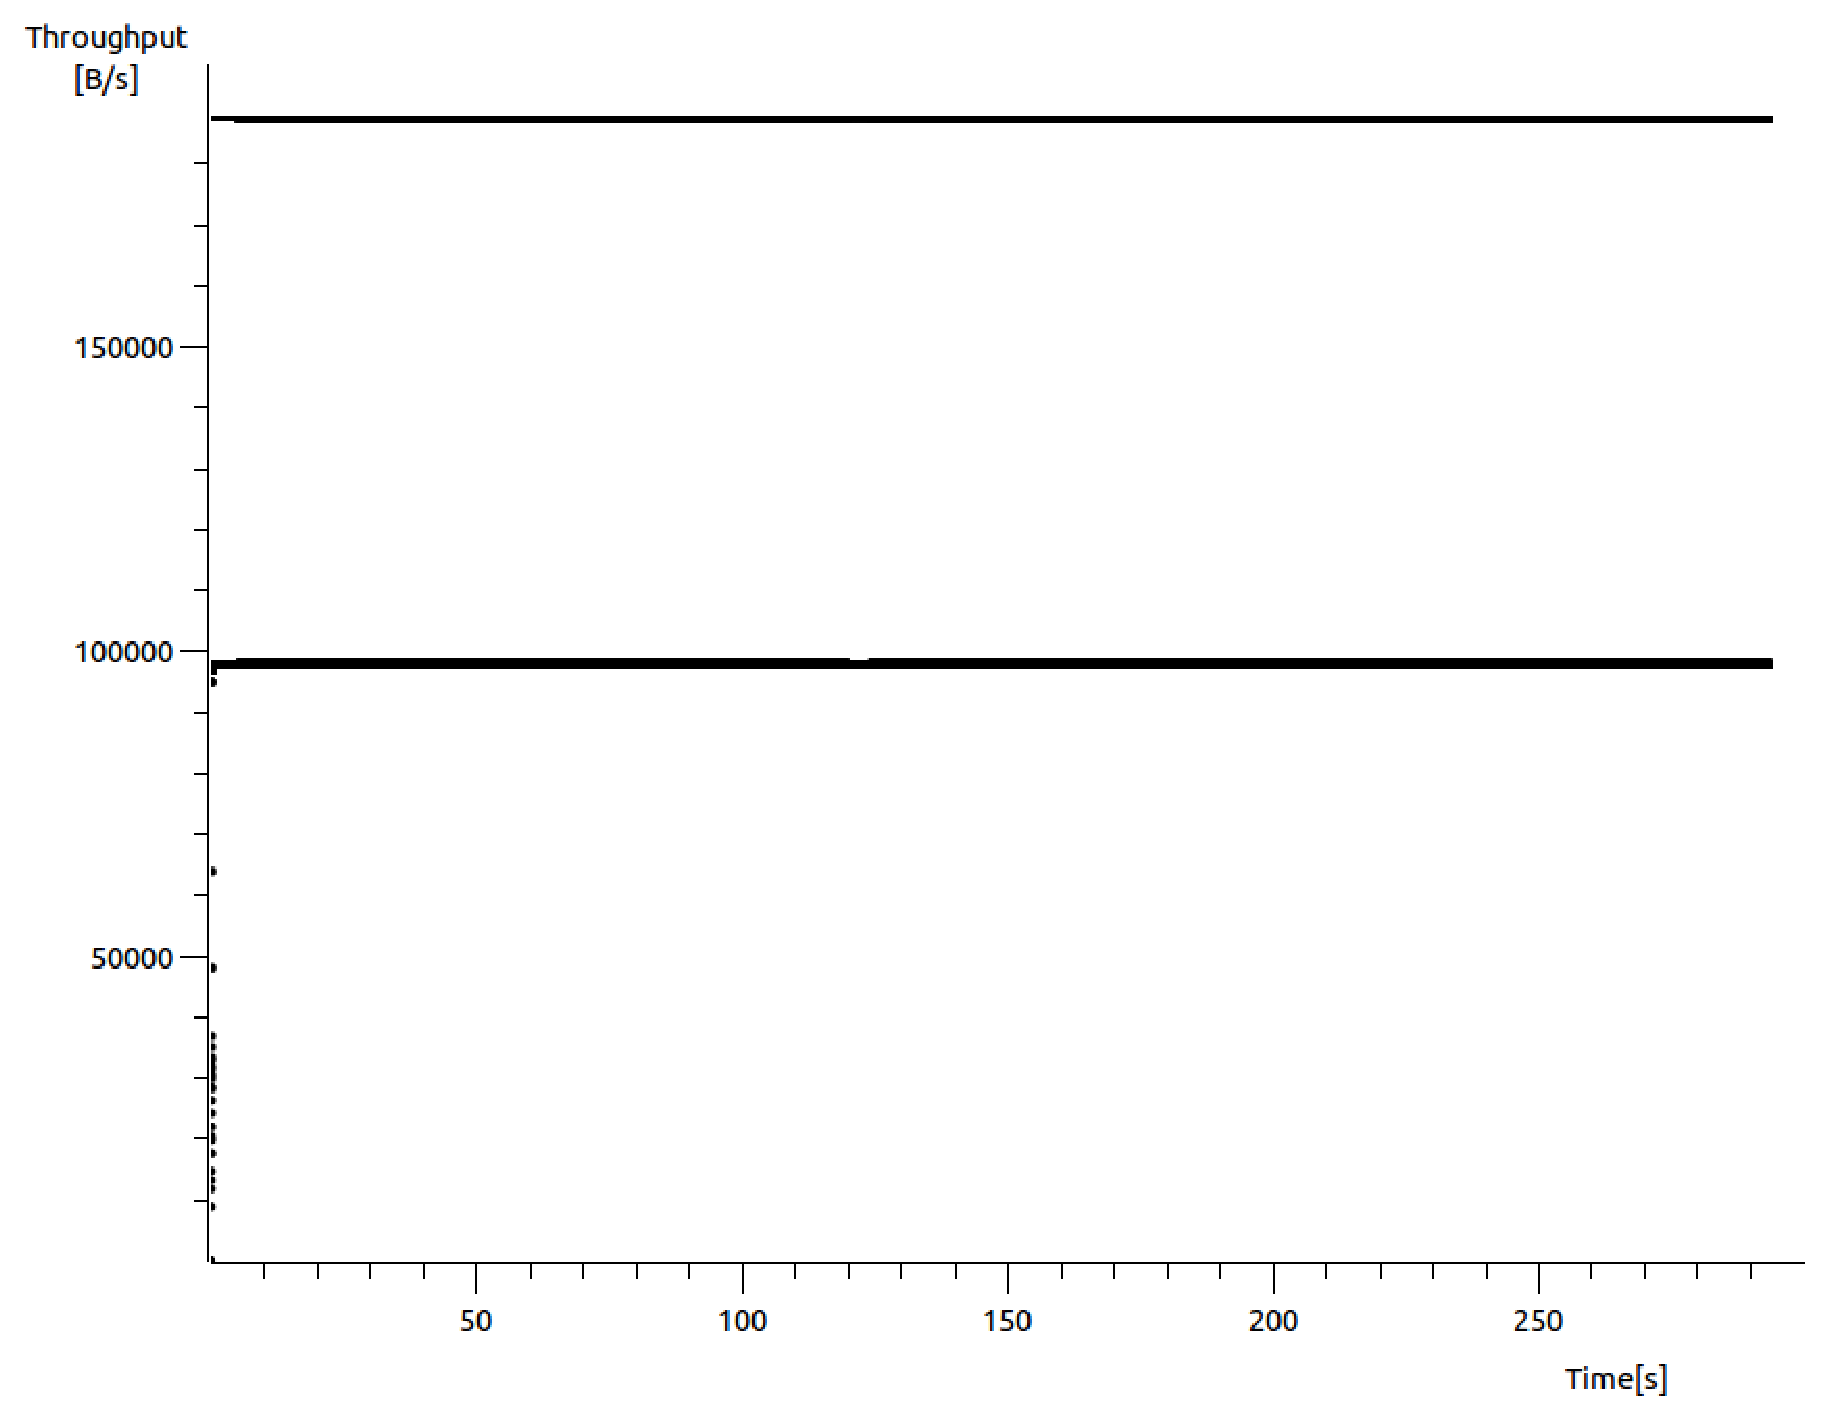
\includegraphics[width=\textwidth]{s1-0_thru}
  \caption{Throughput}
 \end{subfigure}
 \begin{subfigure}[b]{0.2\textwidth}
  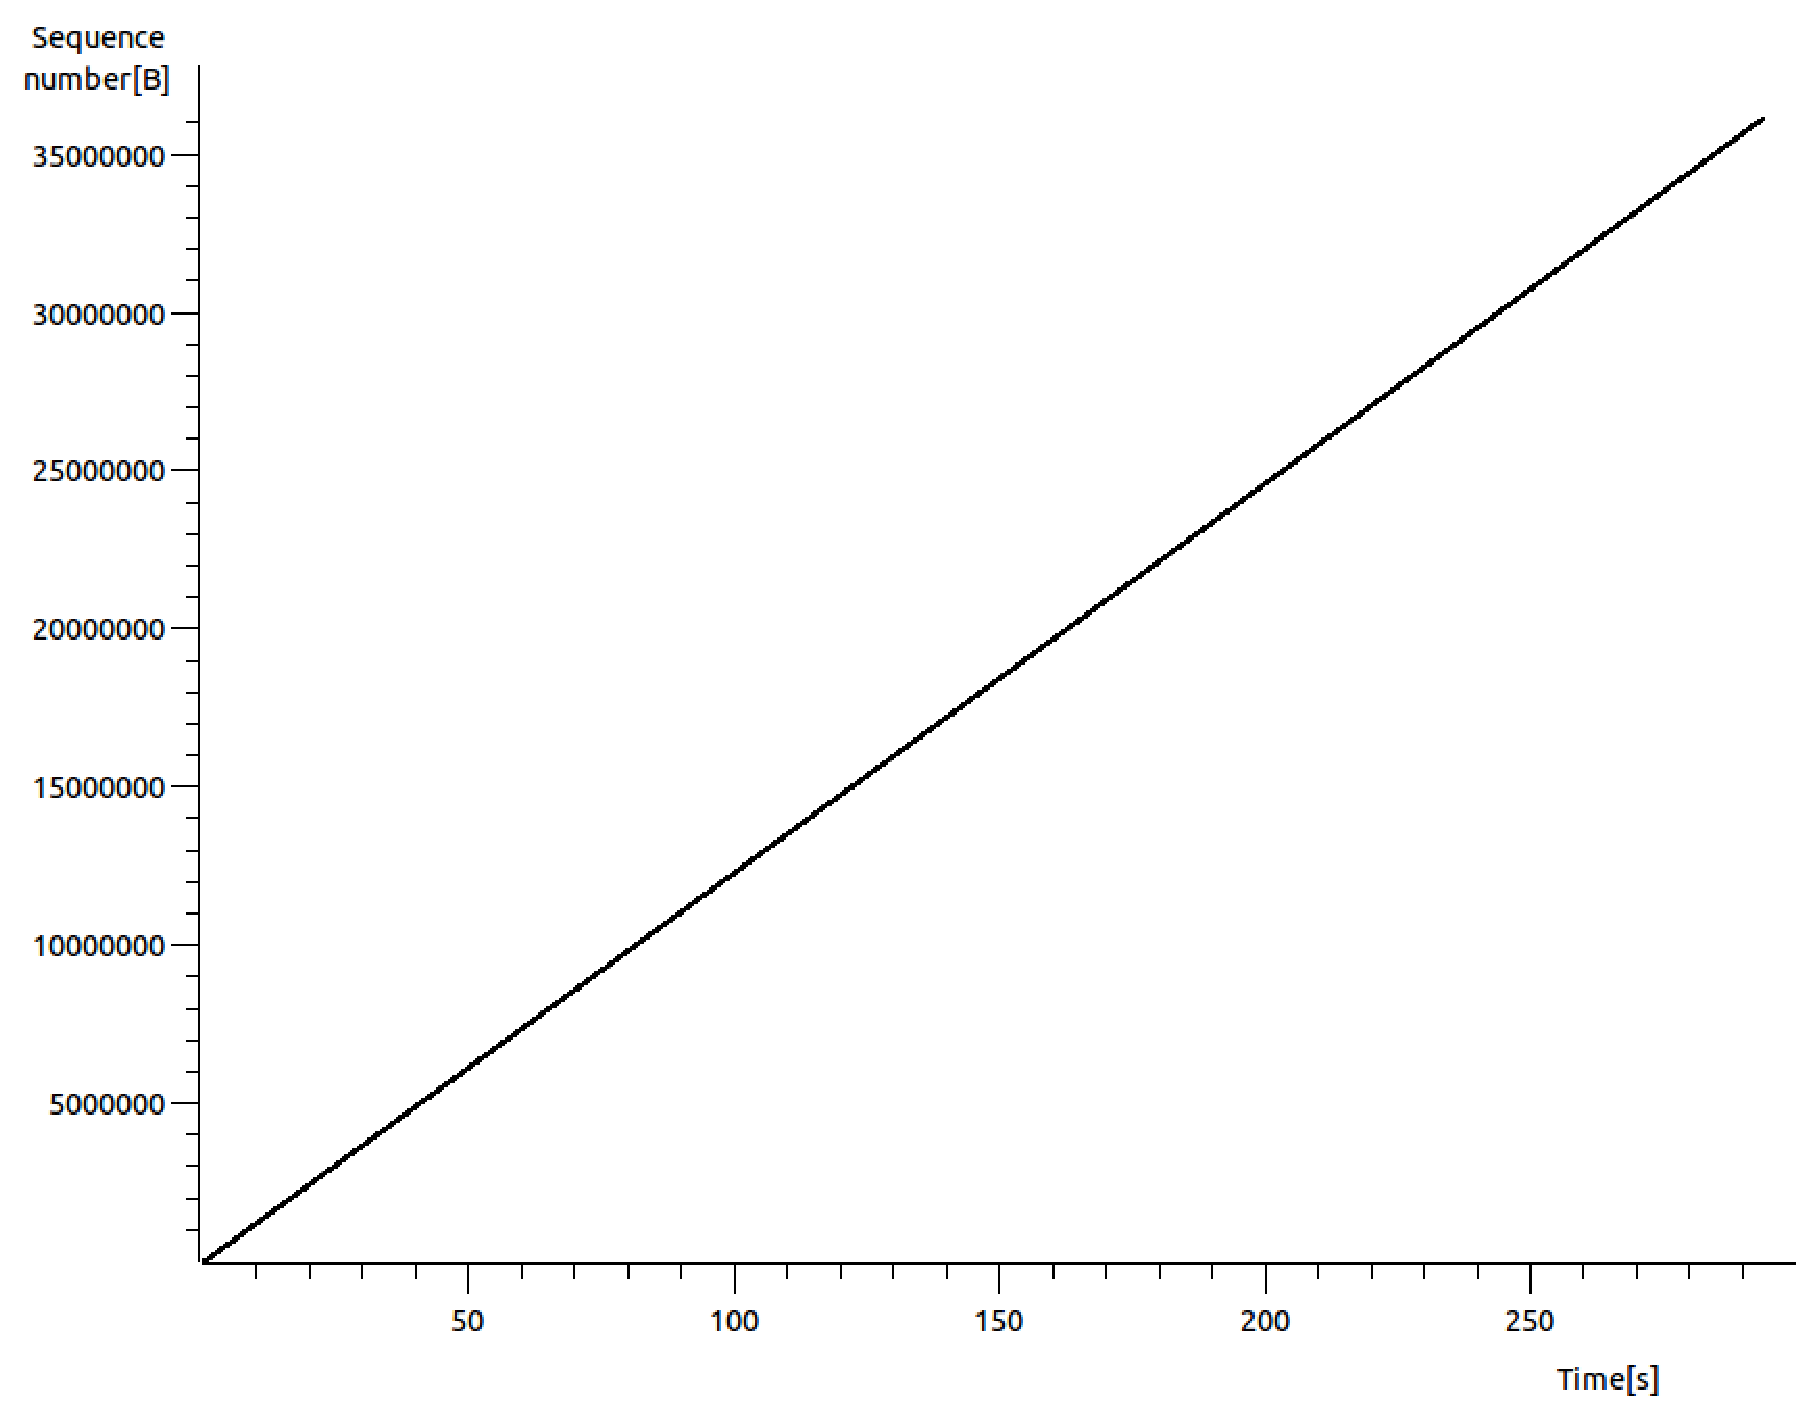
\includegraphics[width=\textwidth]{s1-0_seq}
  \caption{TCP sequence}
 \end{subfigure}
 \begin{subfigure}[b]{0.2\textwidth}
  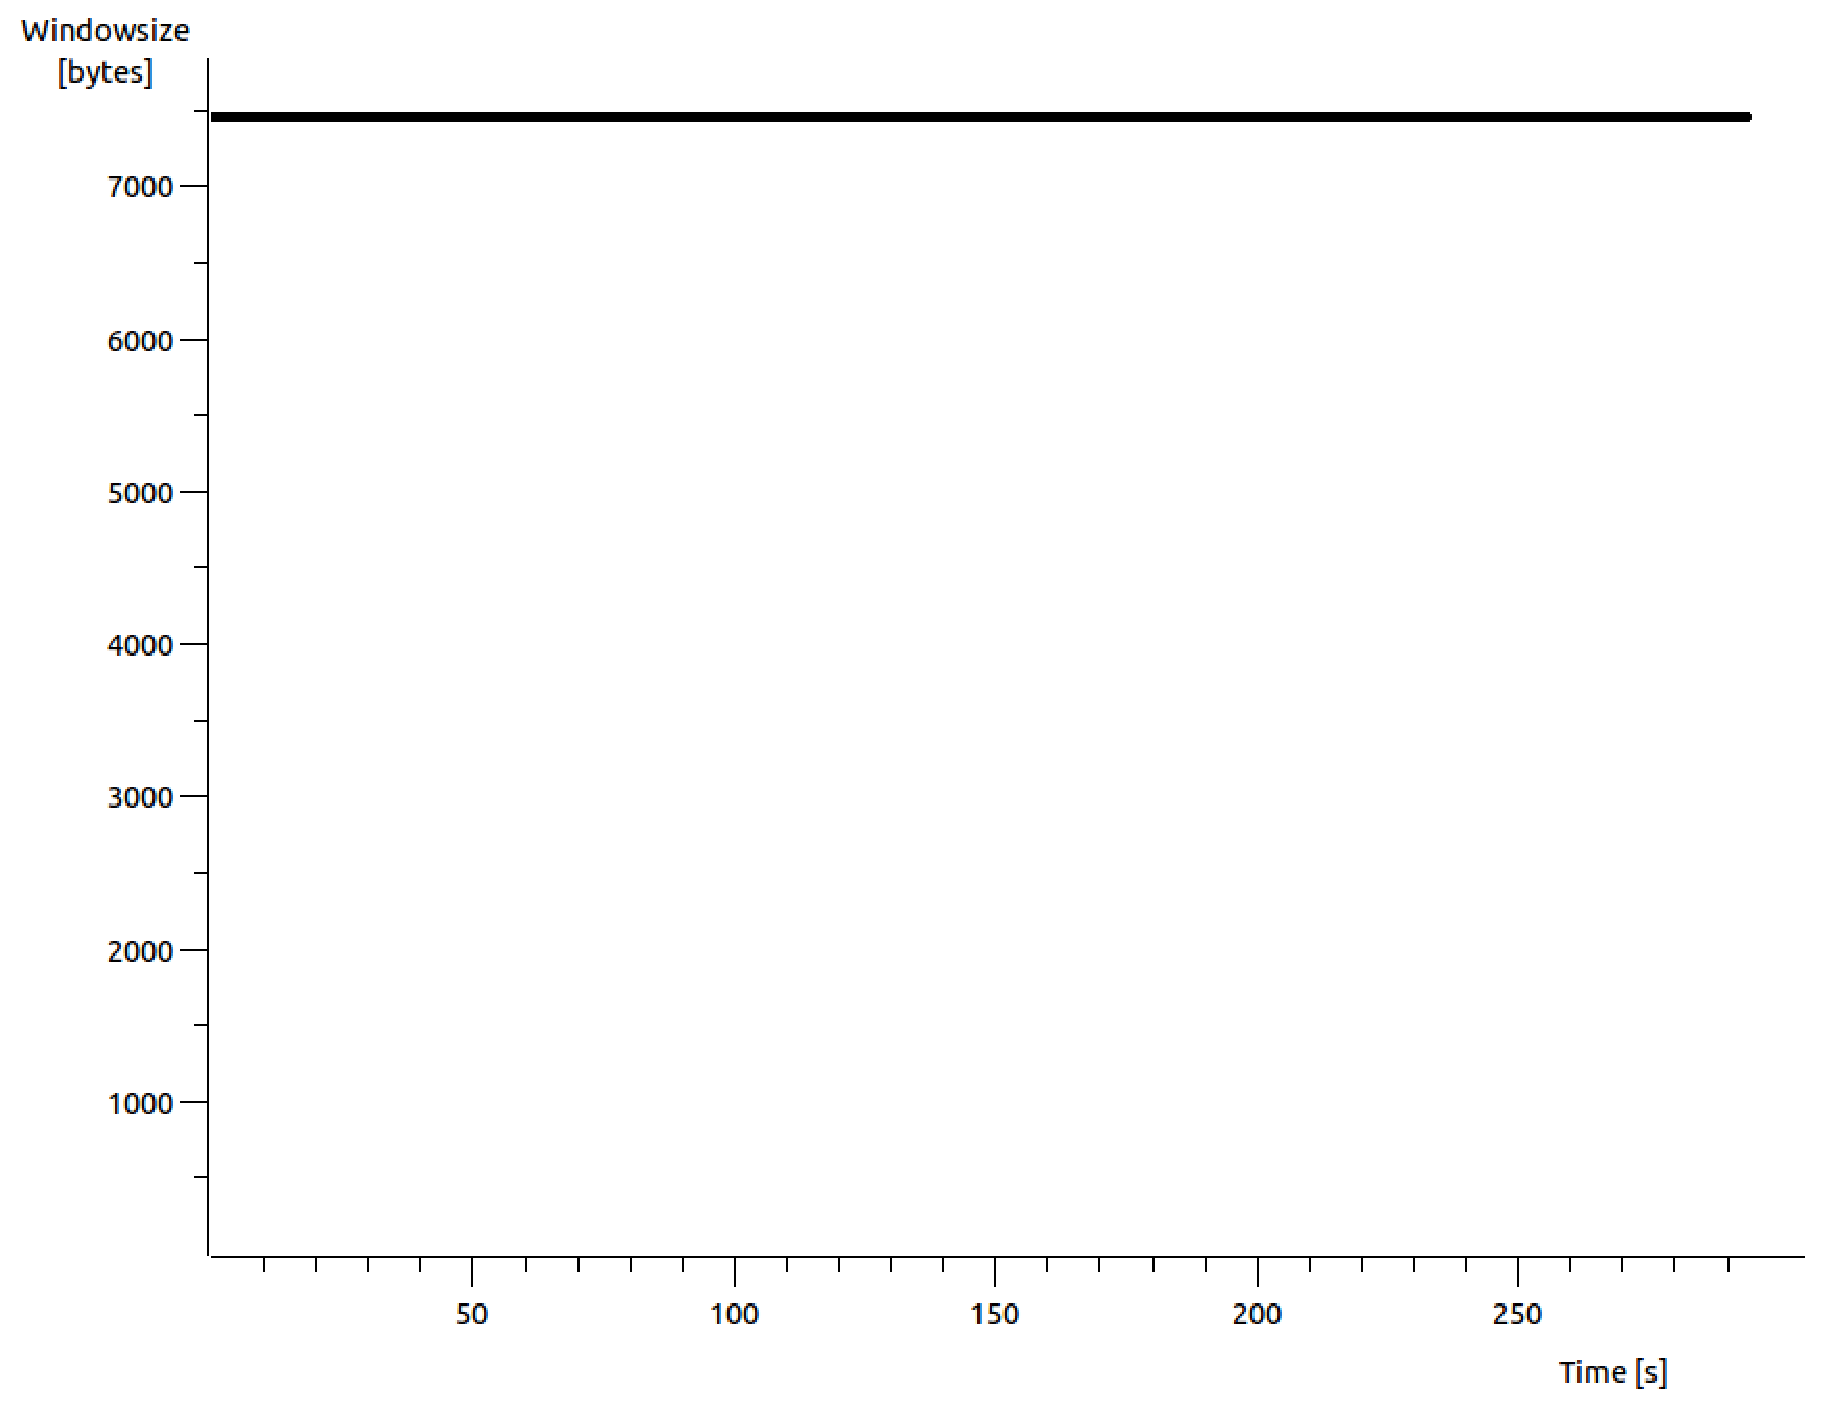
\includegraphics[width=\textwidth]{s1-0_wnd}
  \caption{Window size}
 \end{subfigure}
 \begin{subfigure}[b]{0.2\textwidth}
  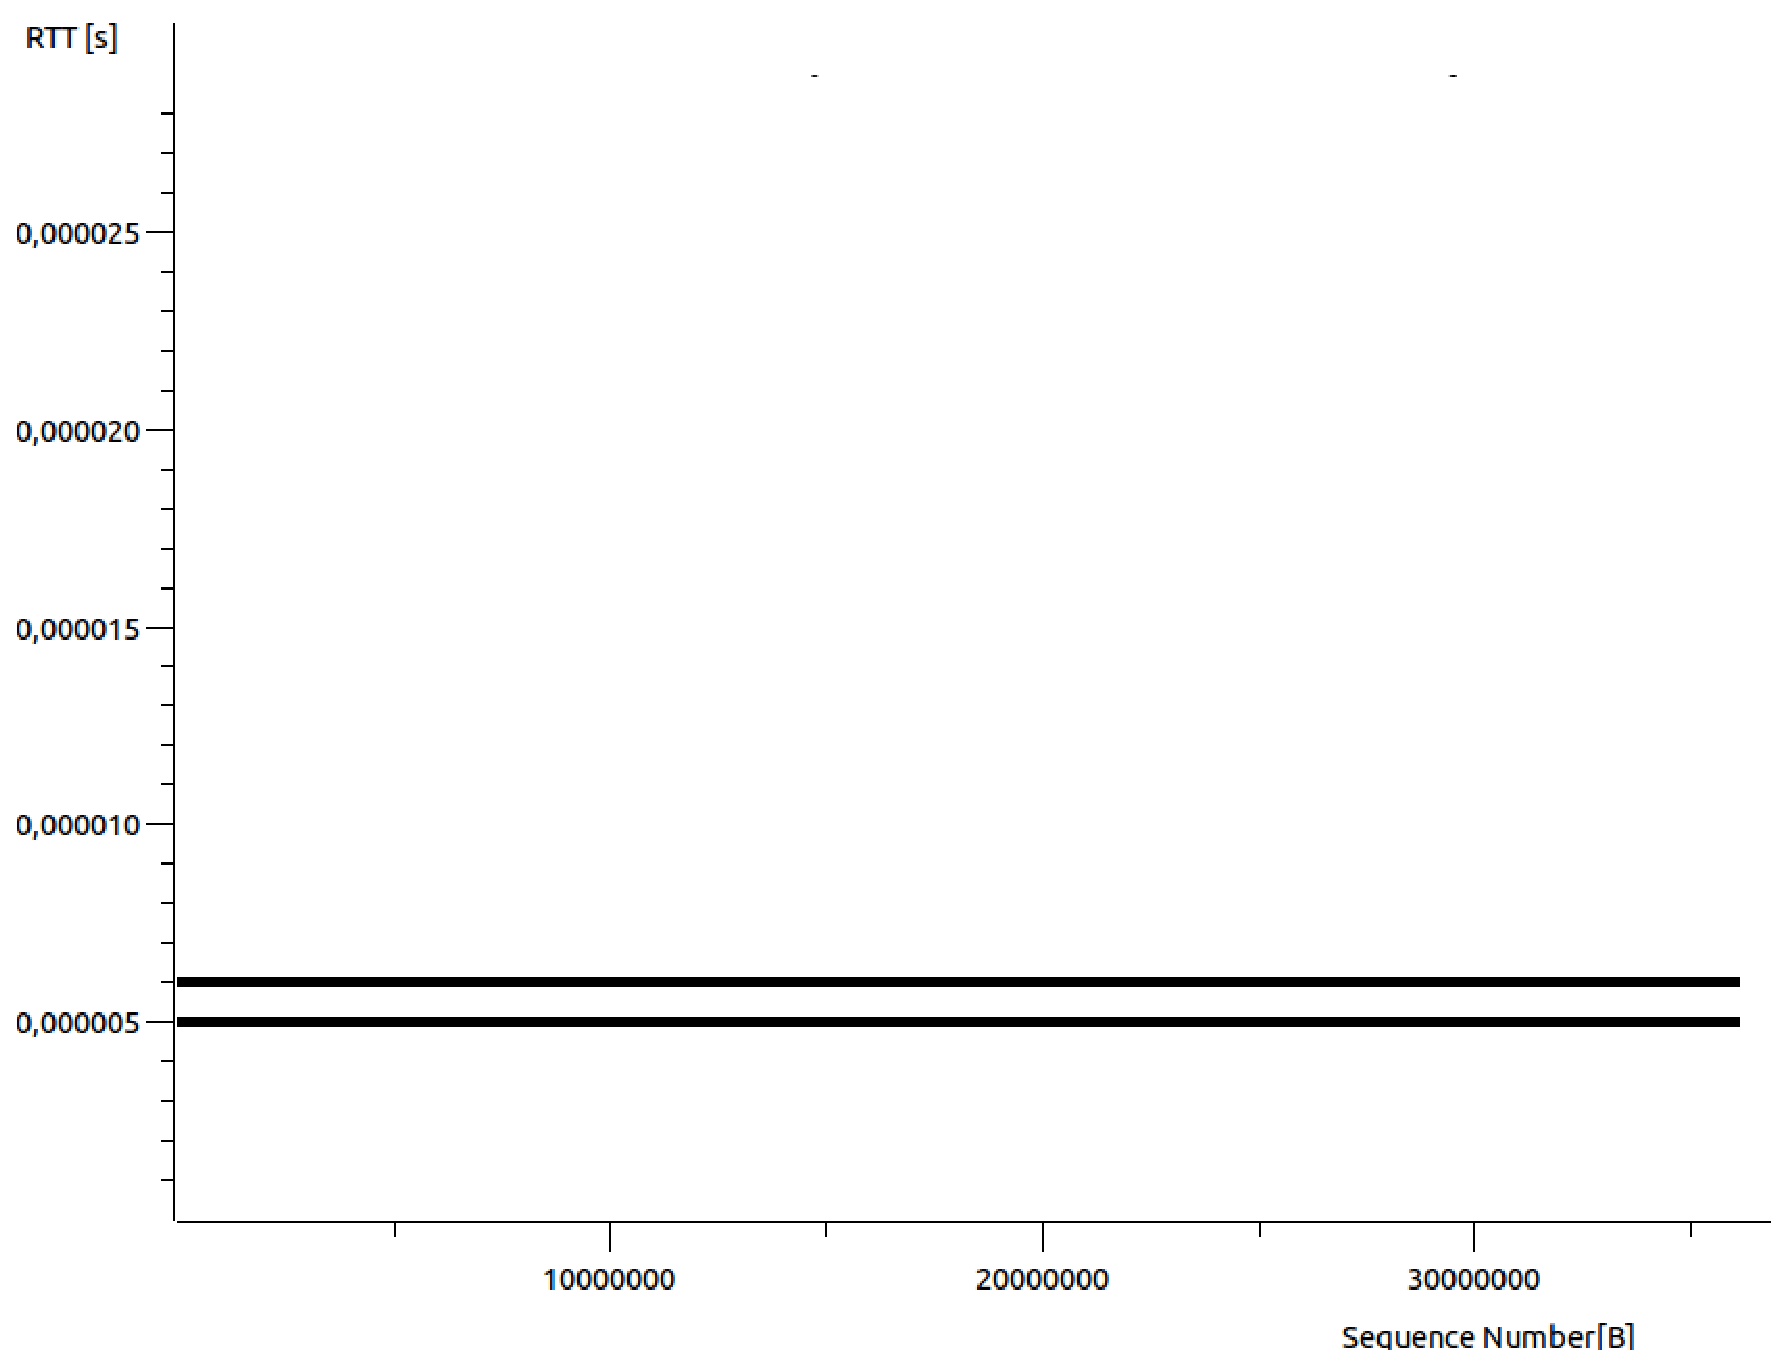
\includegraphics[width=\textwidth]{s1-0_rtt}
  \caption{RTT}
 \end{subfigure}
 \caption{Scene 1-0: TCP Reno + 10 ms delay}
\end{figure}

\begin{figure}
 \centering
 \begin{subfigure}[b]{0.2\textwidth}
  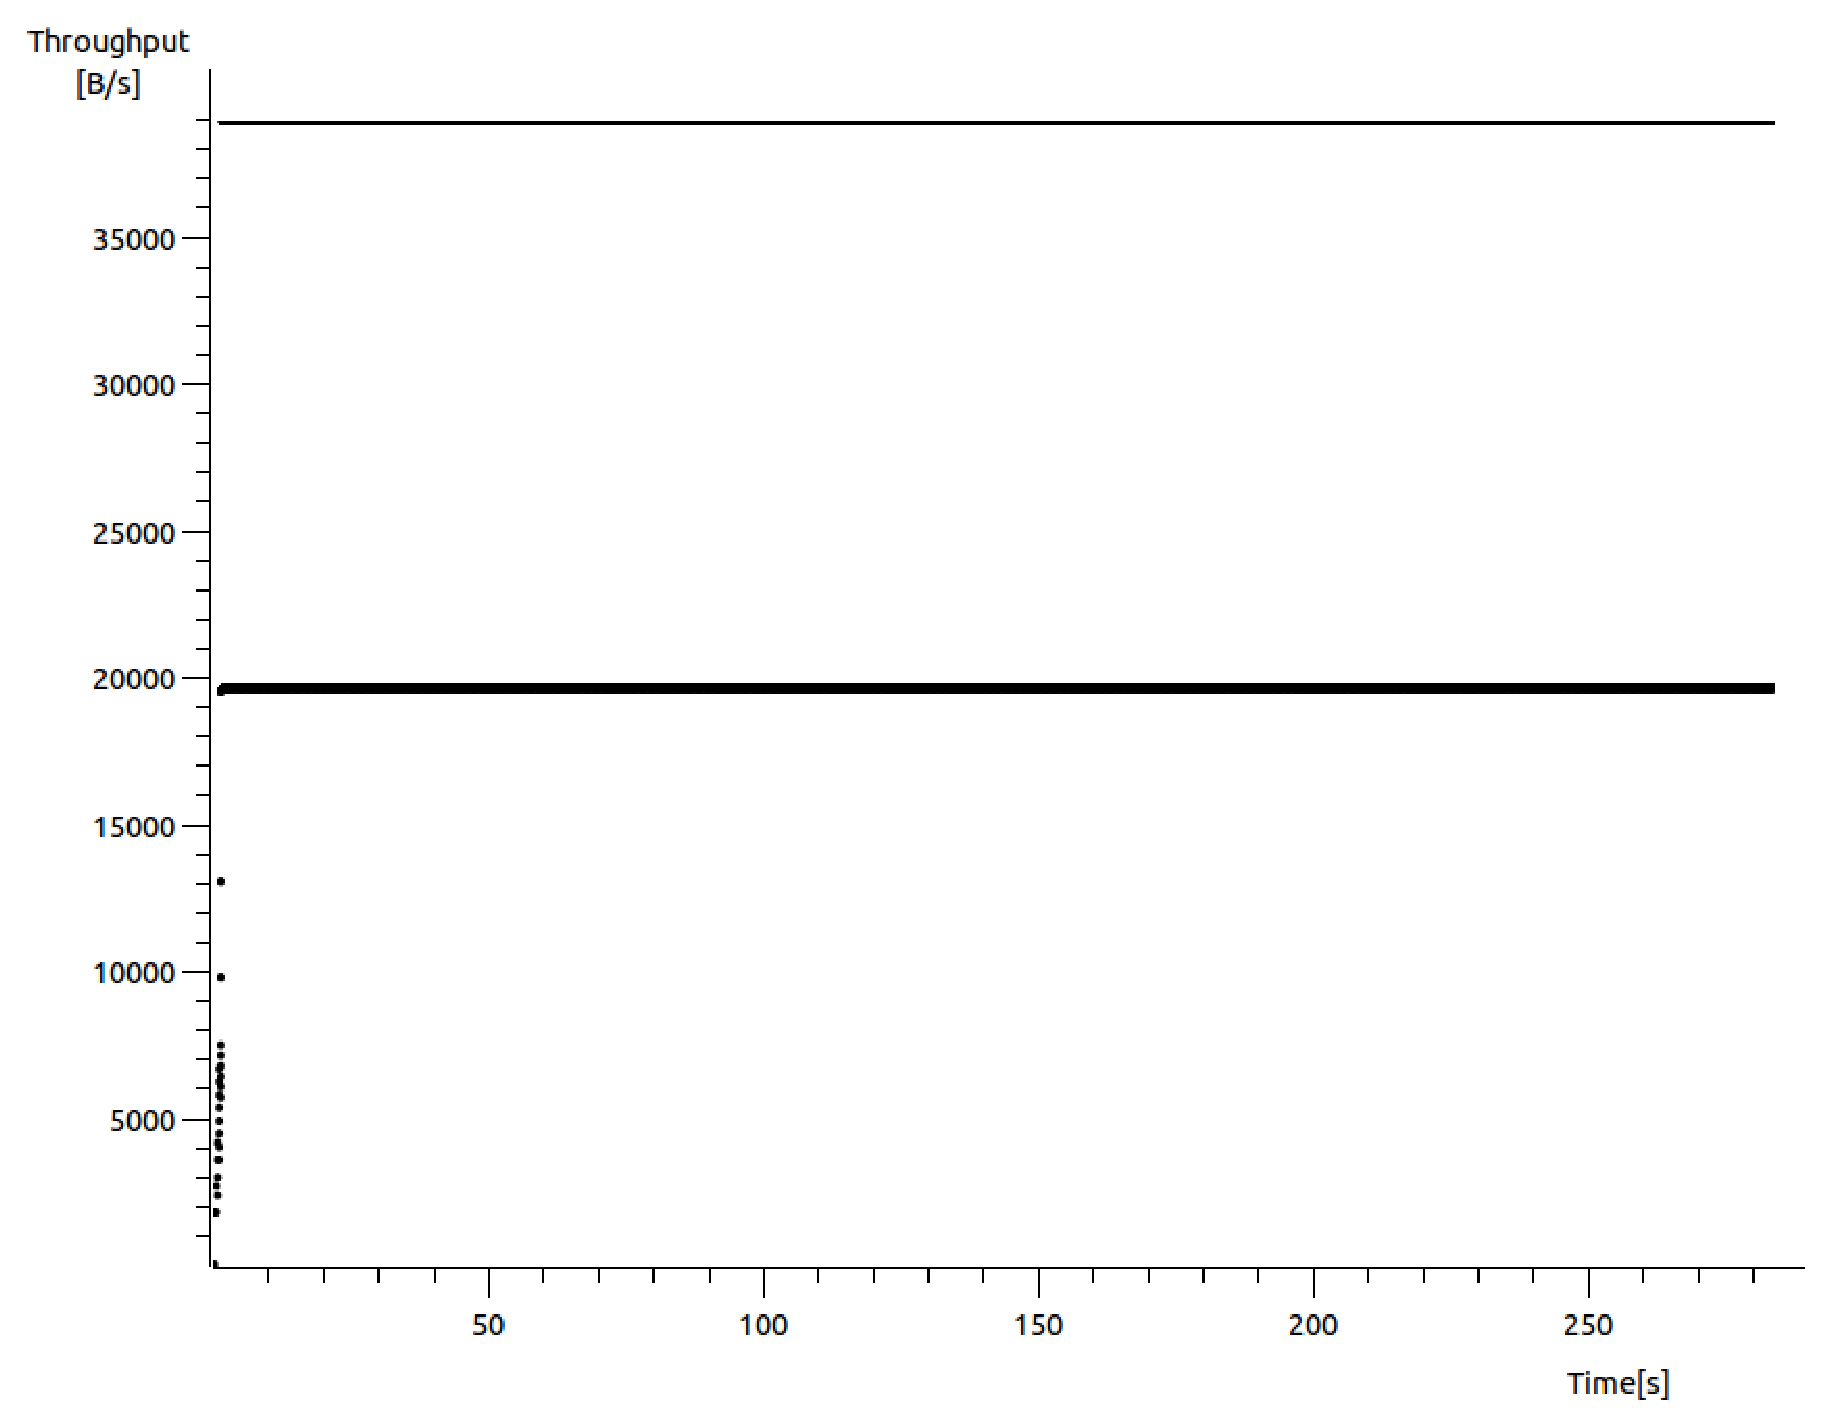
\includegraphics[width=\textwidth]{s1-1_thru}
  \caption{Throughput}
 \end{subfigure}
 \begin{subfigure}[b]{0.2\textwidth}
  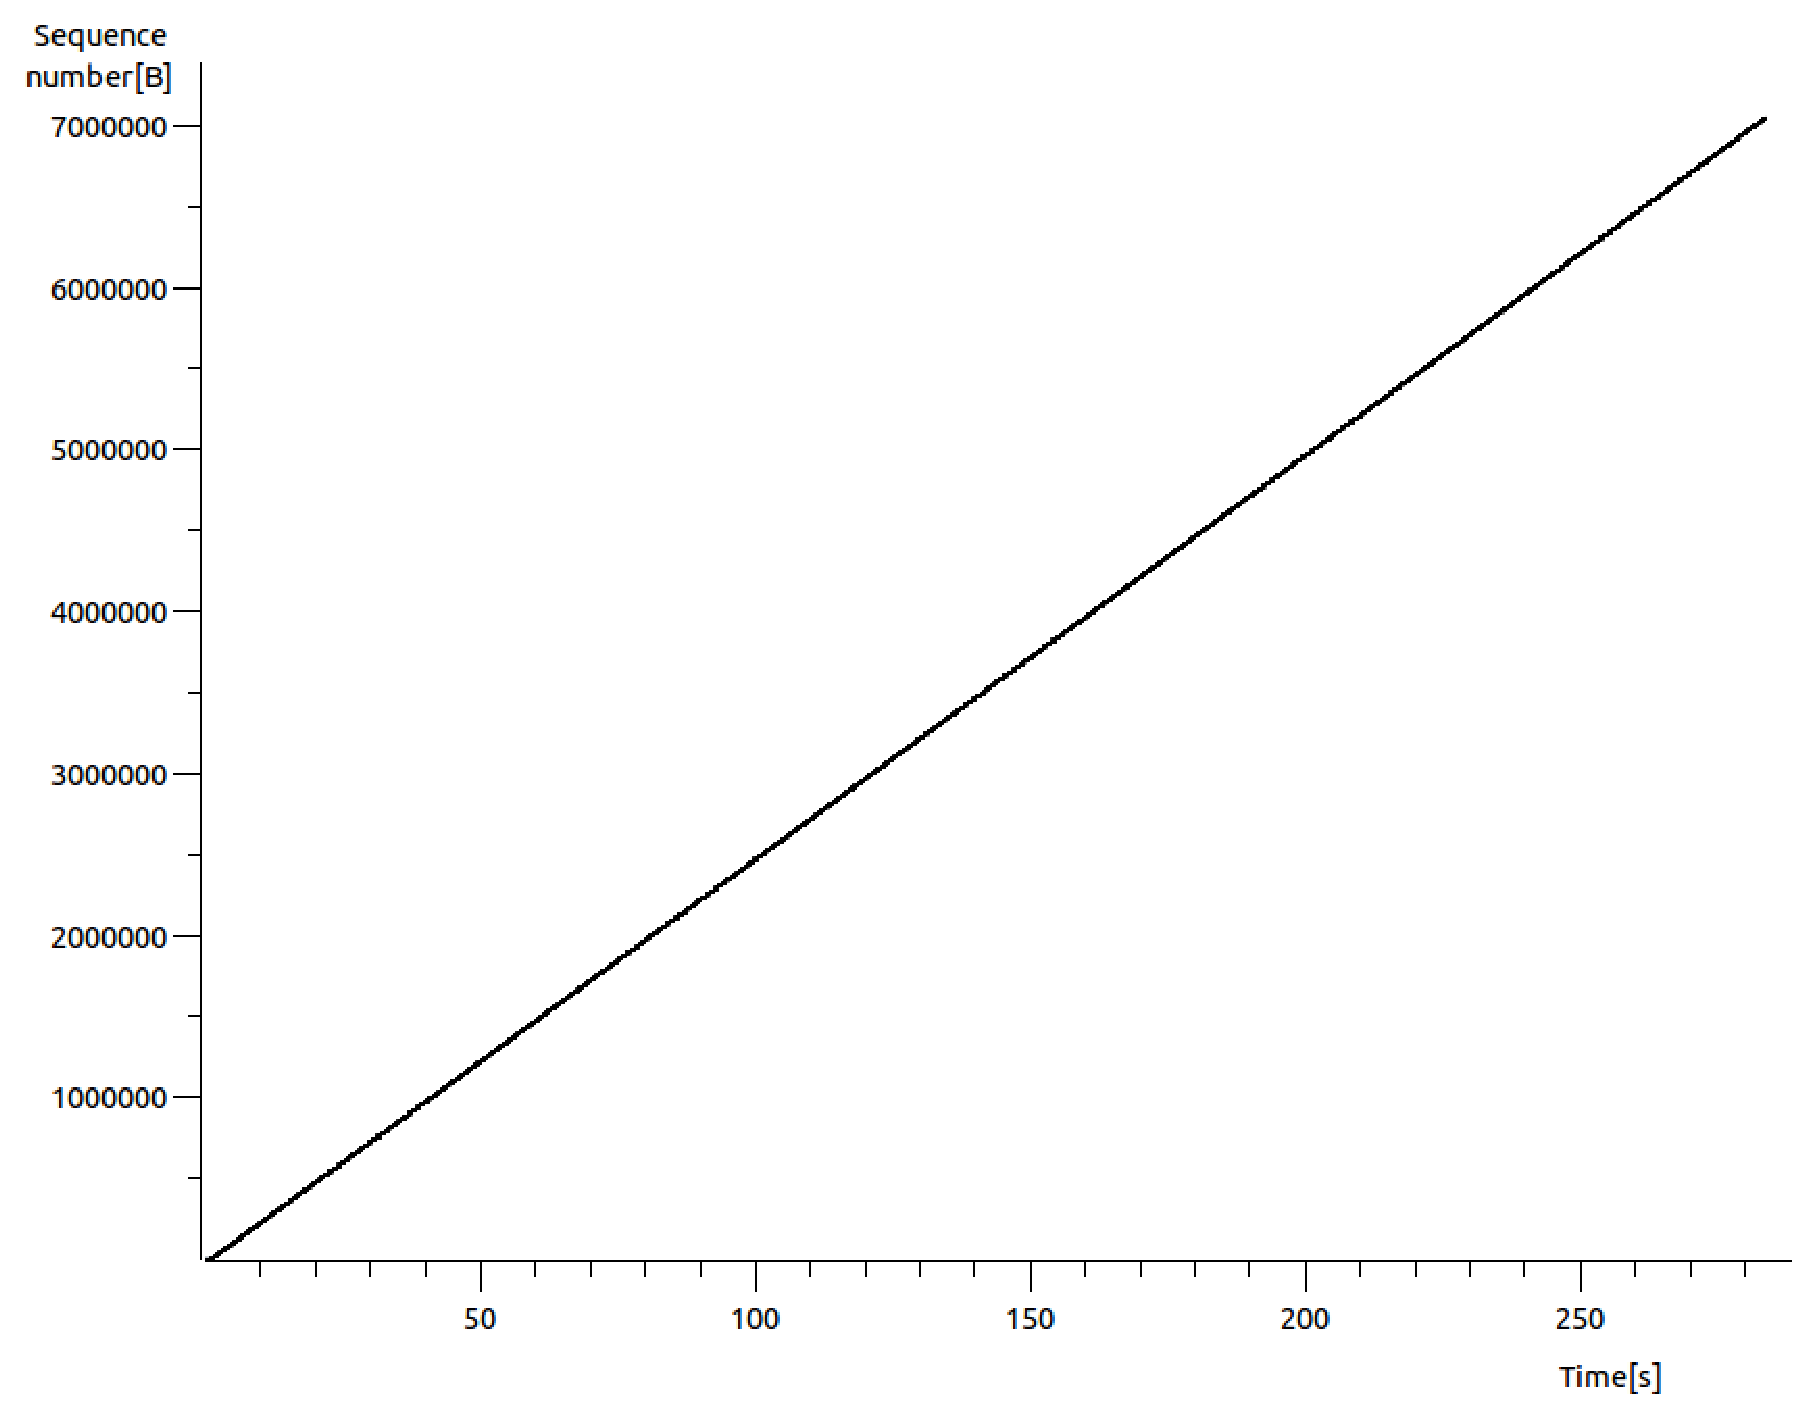
\includegraphics[width=\textwidth]{s1-1_seq}
  \caption{TCP sequence}
 \end{subfigure}
 \begin{subfigure}[b]{0.2\textwidth}
  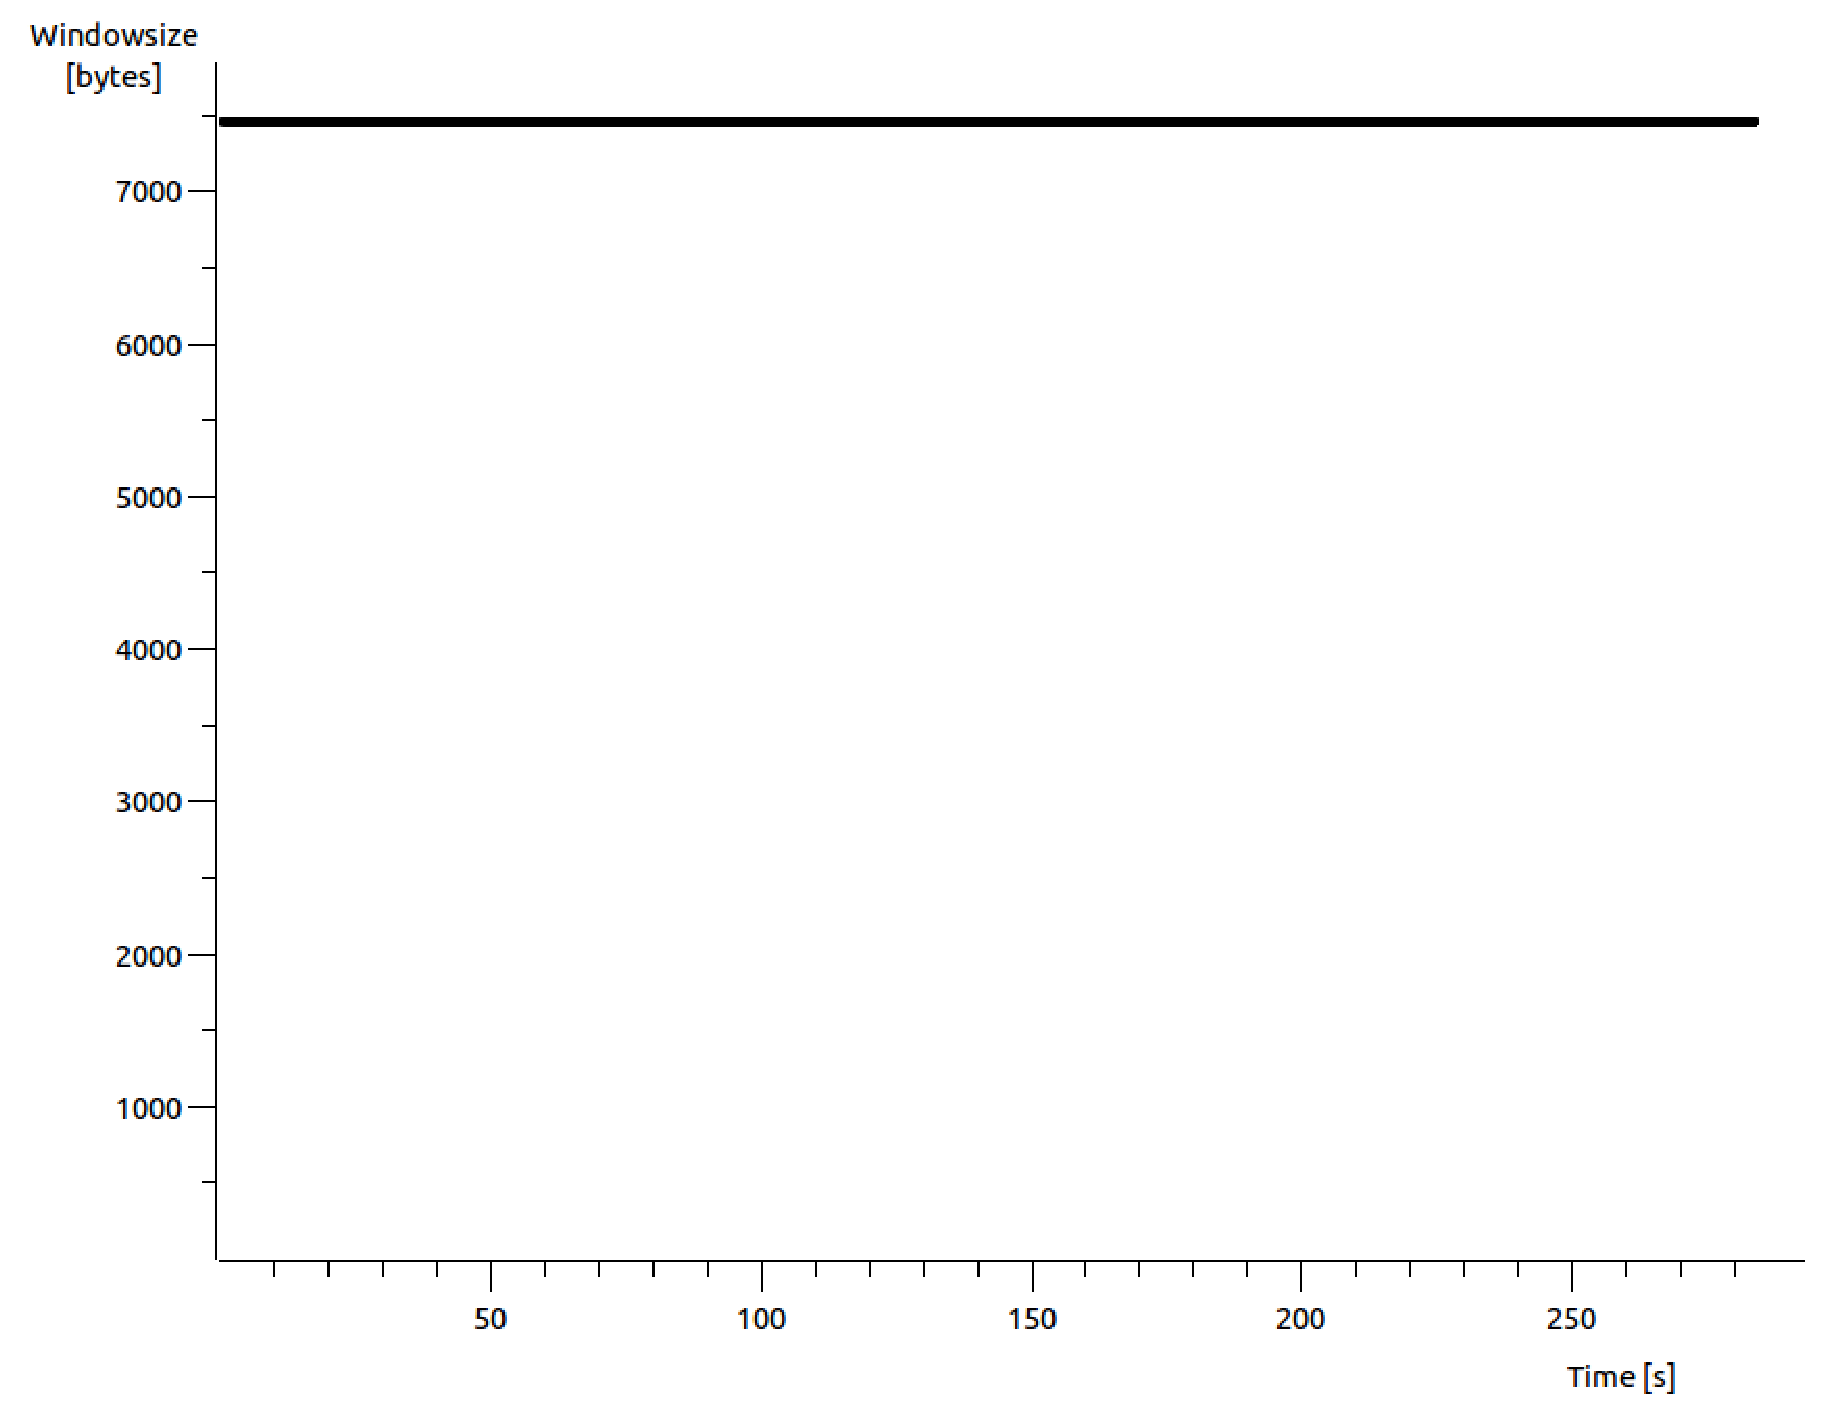
\includegraphics[width=\textwidth]{s1-1_wnd}
  \caption{Window size}
 \end{subfigure}
 \begin{subfigure}[b]{0.2\textwidth}
  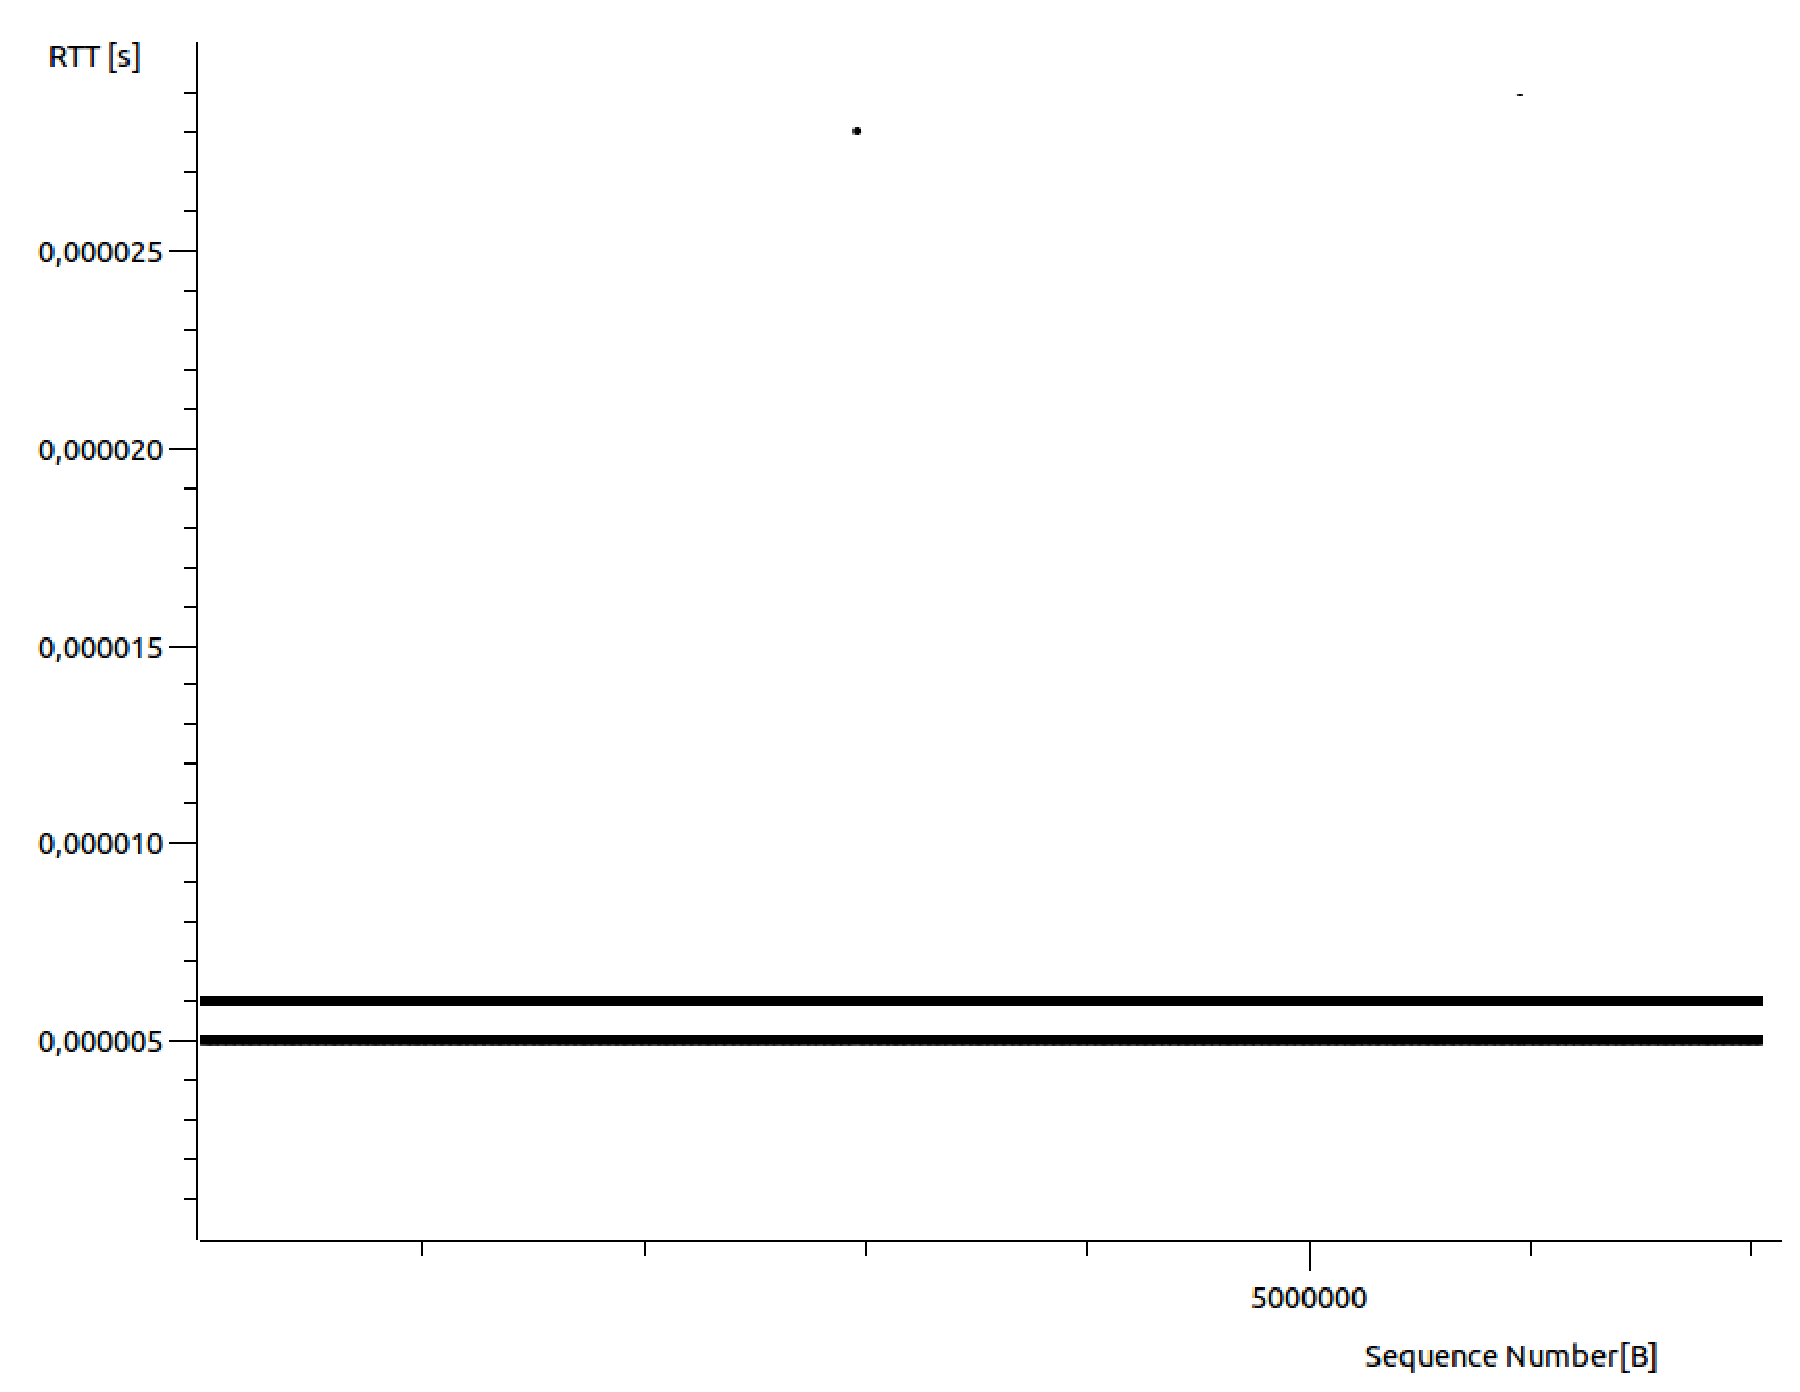
\includegraphics[width=\textwidth]{s1-1_rtt}
  \caption{RTT}
 \end{subfigure}
 \caption{Scene 1-1: TCP Reno + 50 ms delay}
\end{figure}

\begin{figure}
 \centering
 \begin{subfigure}[b]{0.2\textwidth}
  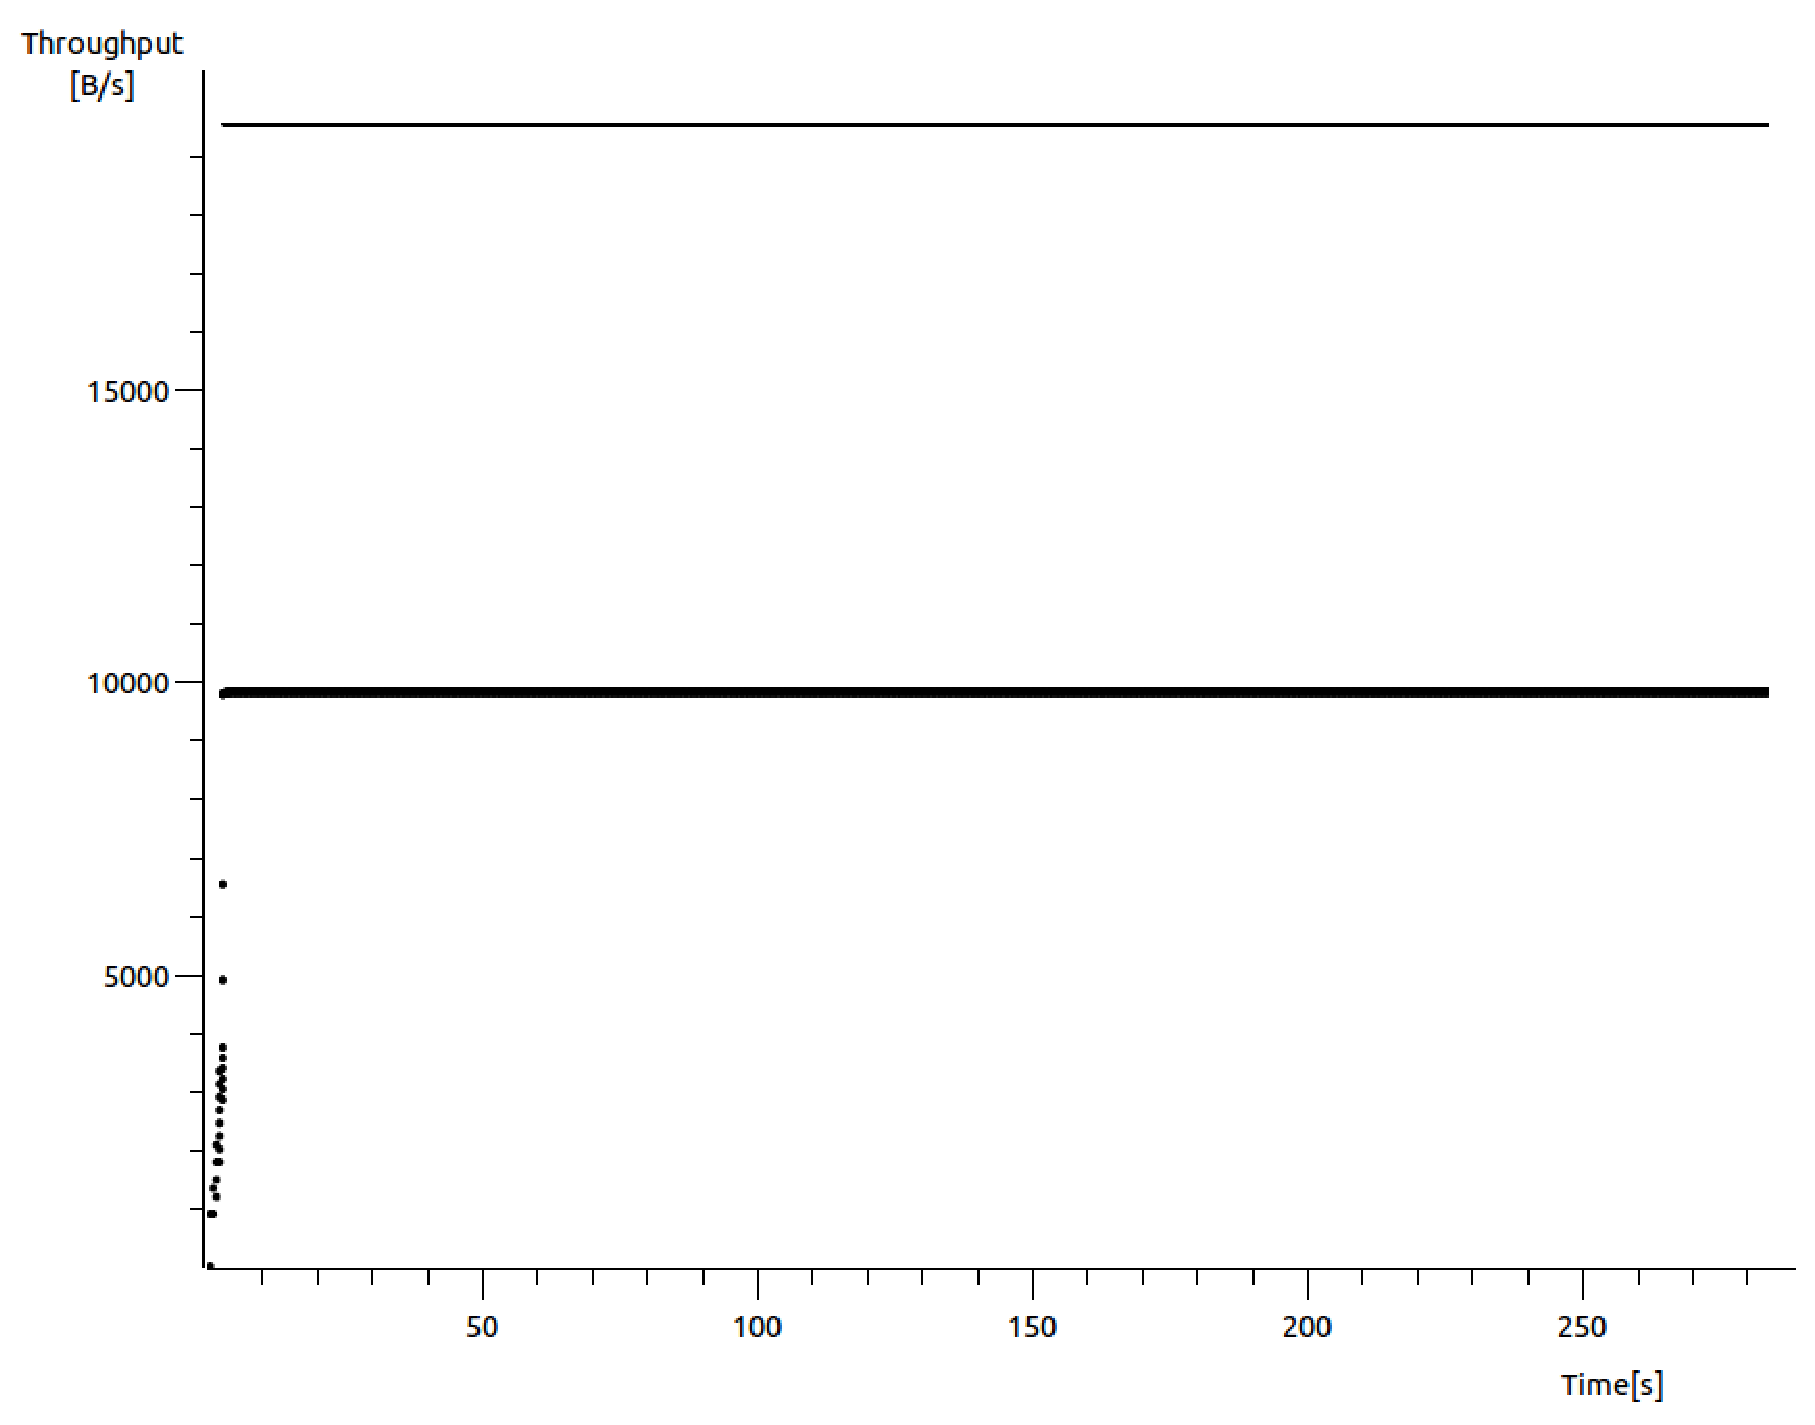
\includegraphics[width=\textwidth]{s1-2_thru}
  \caption{Throughput}
 \end{subfigure}
 \begin{subfigure}[b]{0.2\textwidth}
  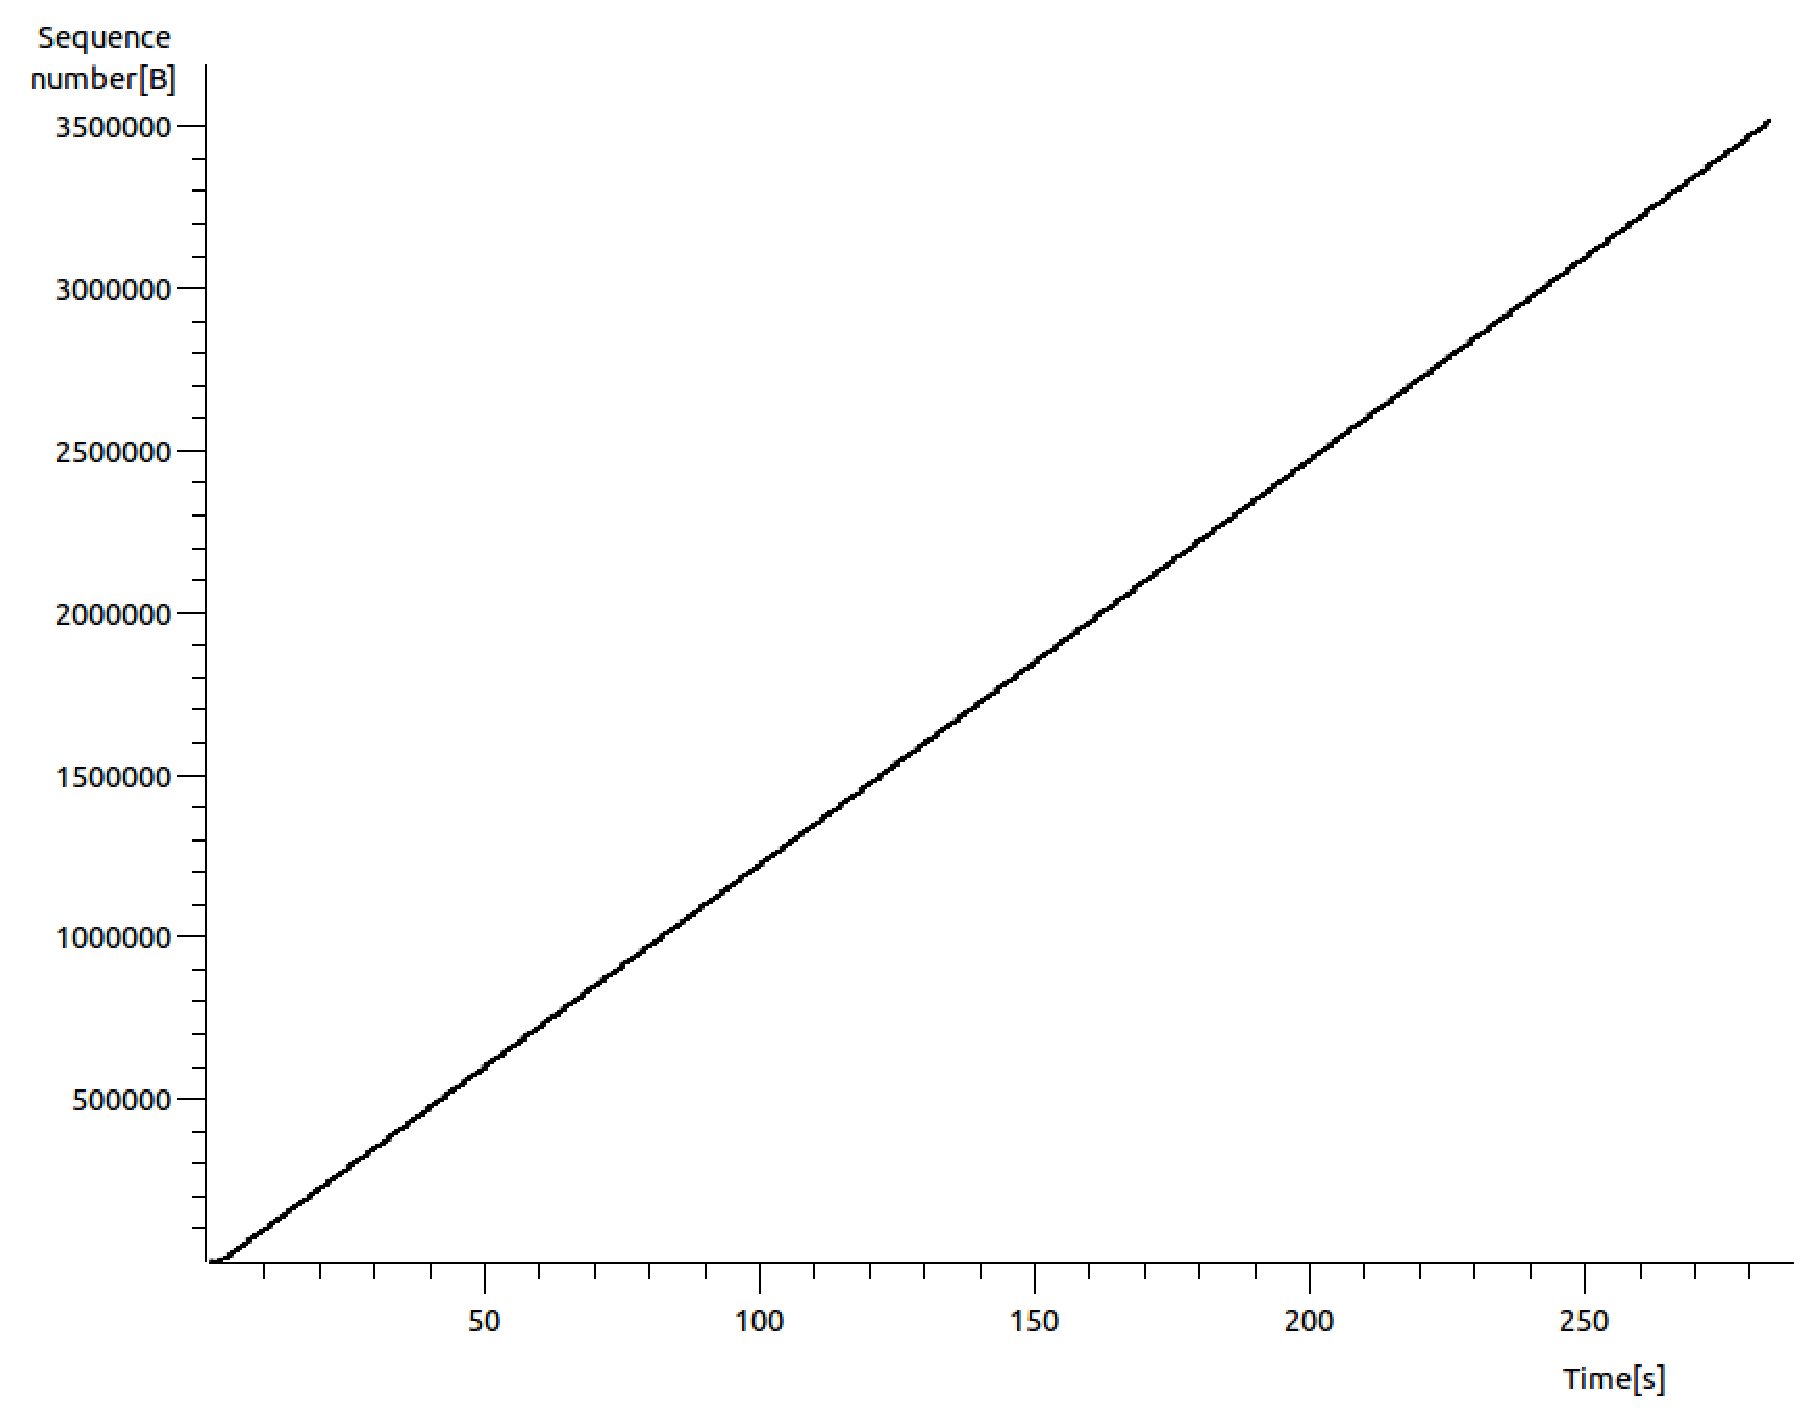
\includegraphics[width=\textwidth]{s1-2_seq}
  \caption{TCP sequence}
 \end{subfigure}
 \begin{subfigure}[b]{0.2\textwidth}
  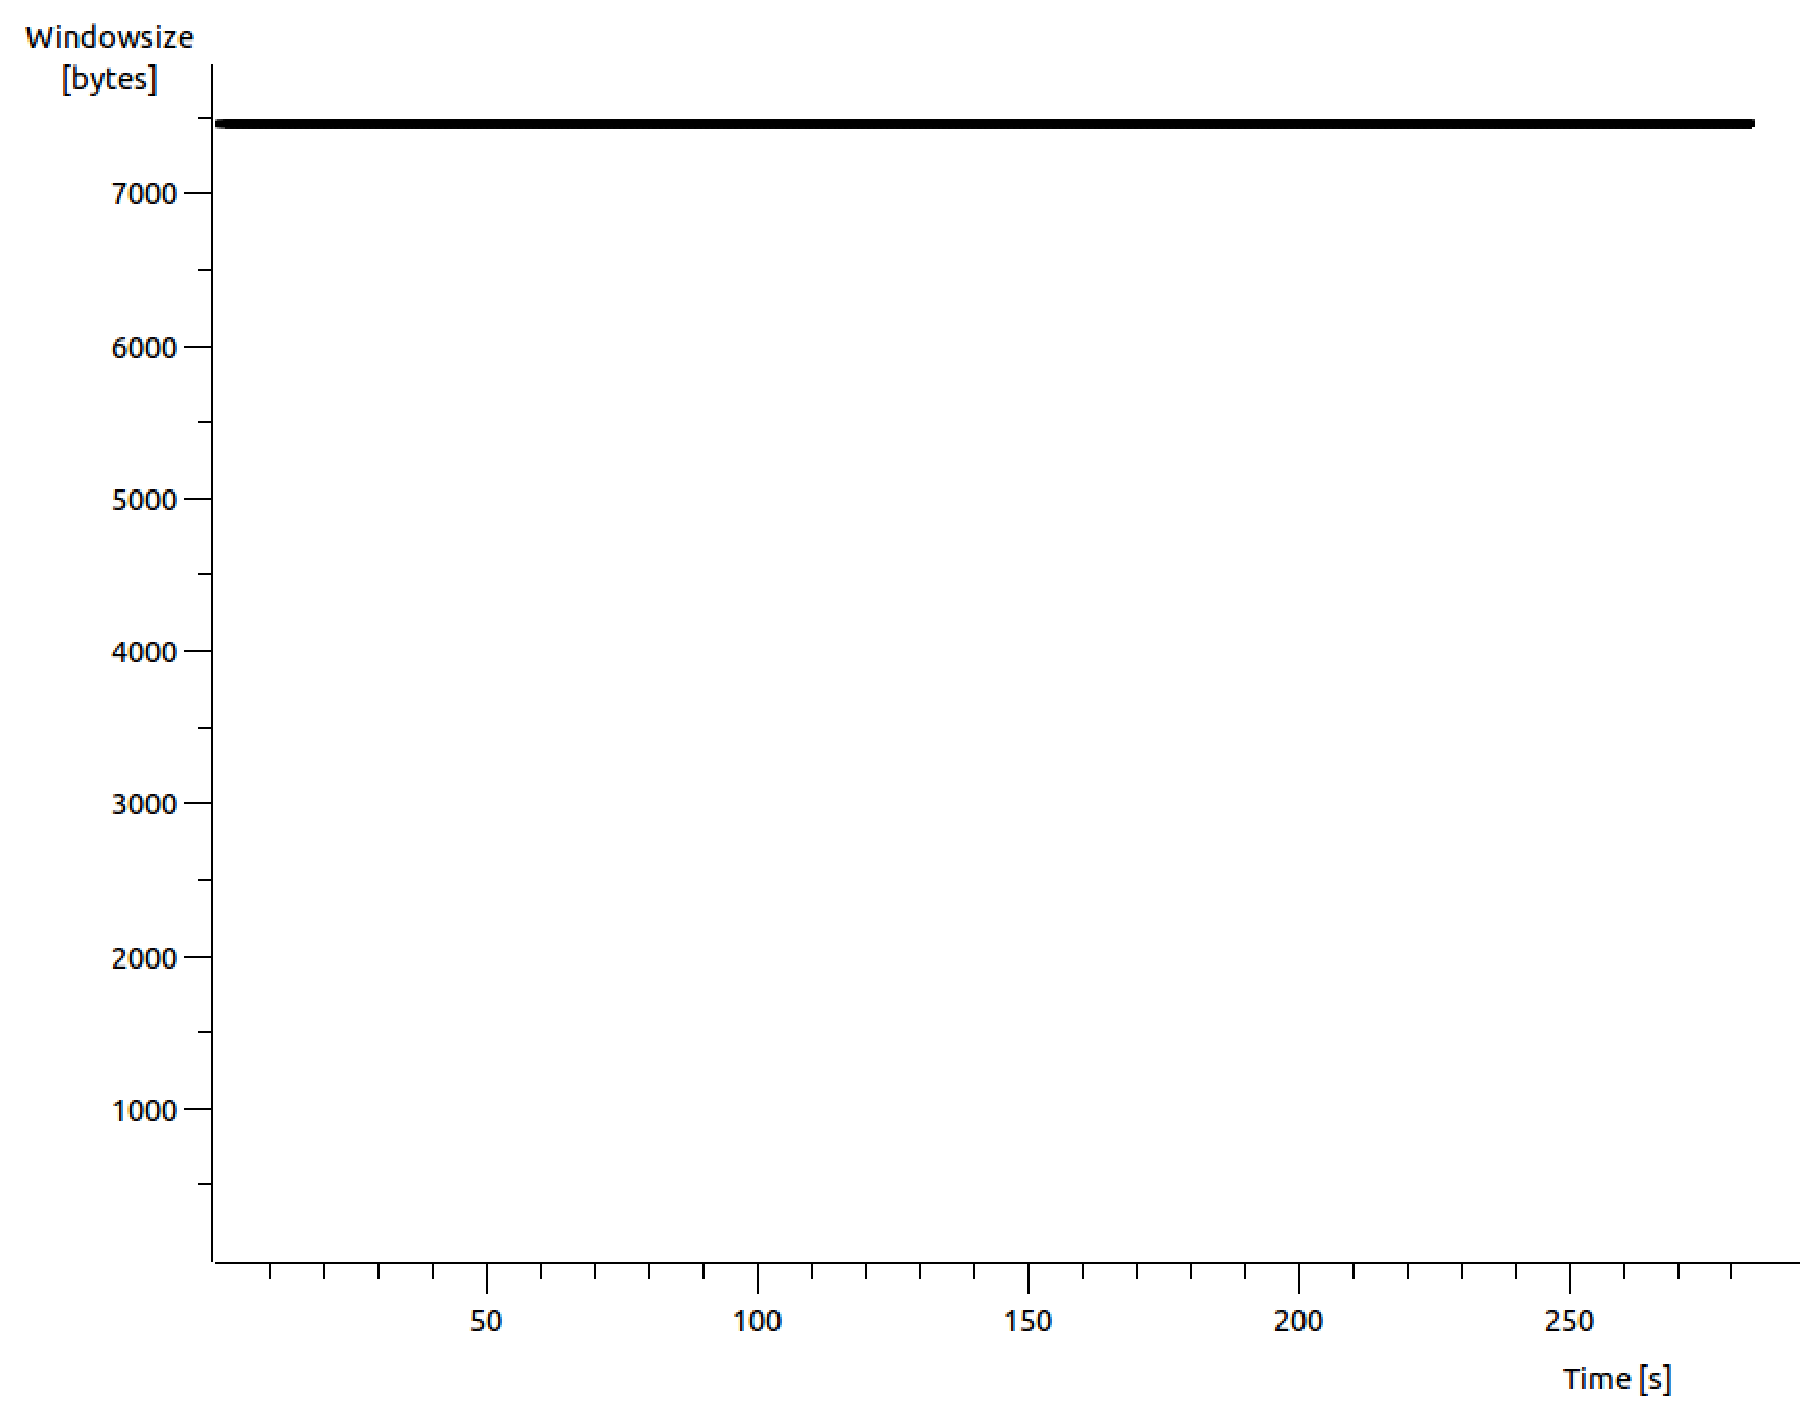
\includegraphics[width=\textwidth]{s1-2_wnd}
  \caption{Window size}
 \end{subfigure}
 \begin{subfigure}[b]{0.2\textwidth}
  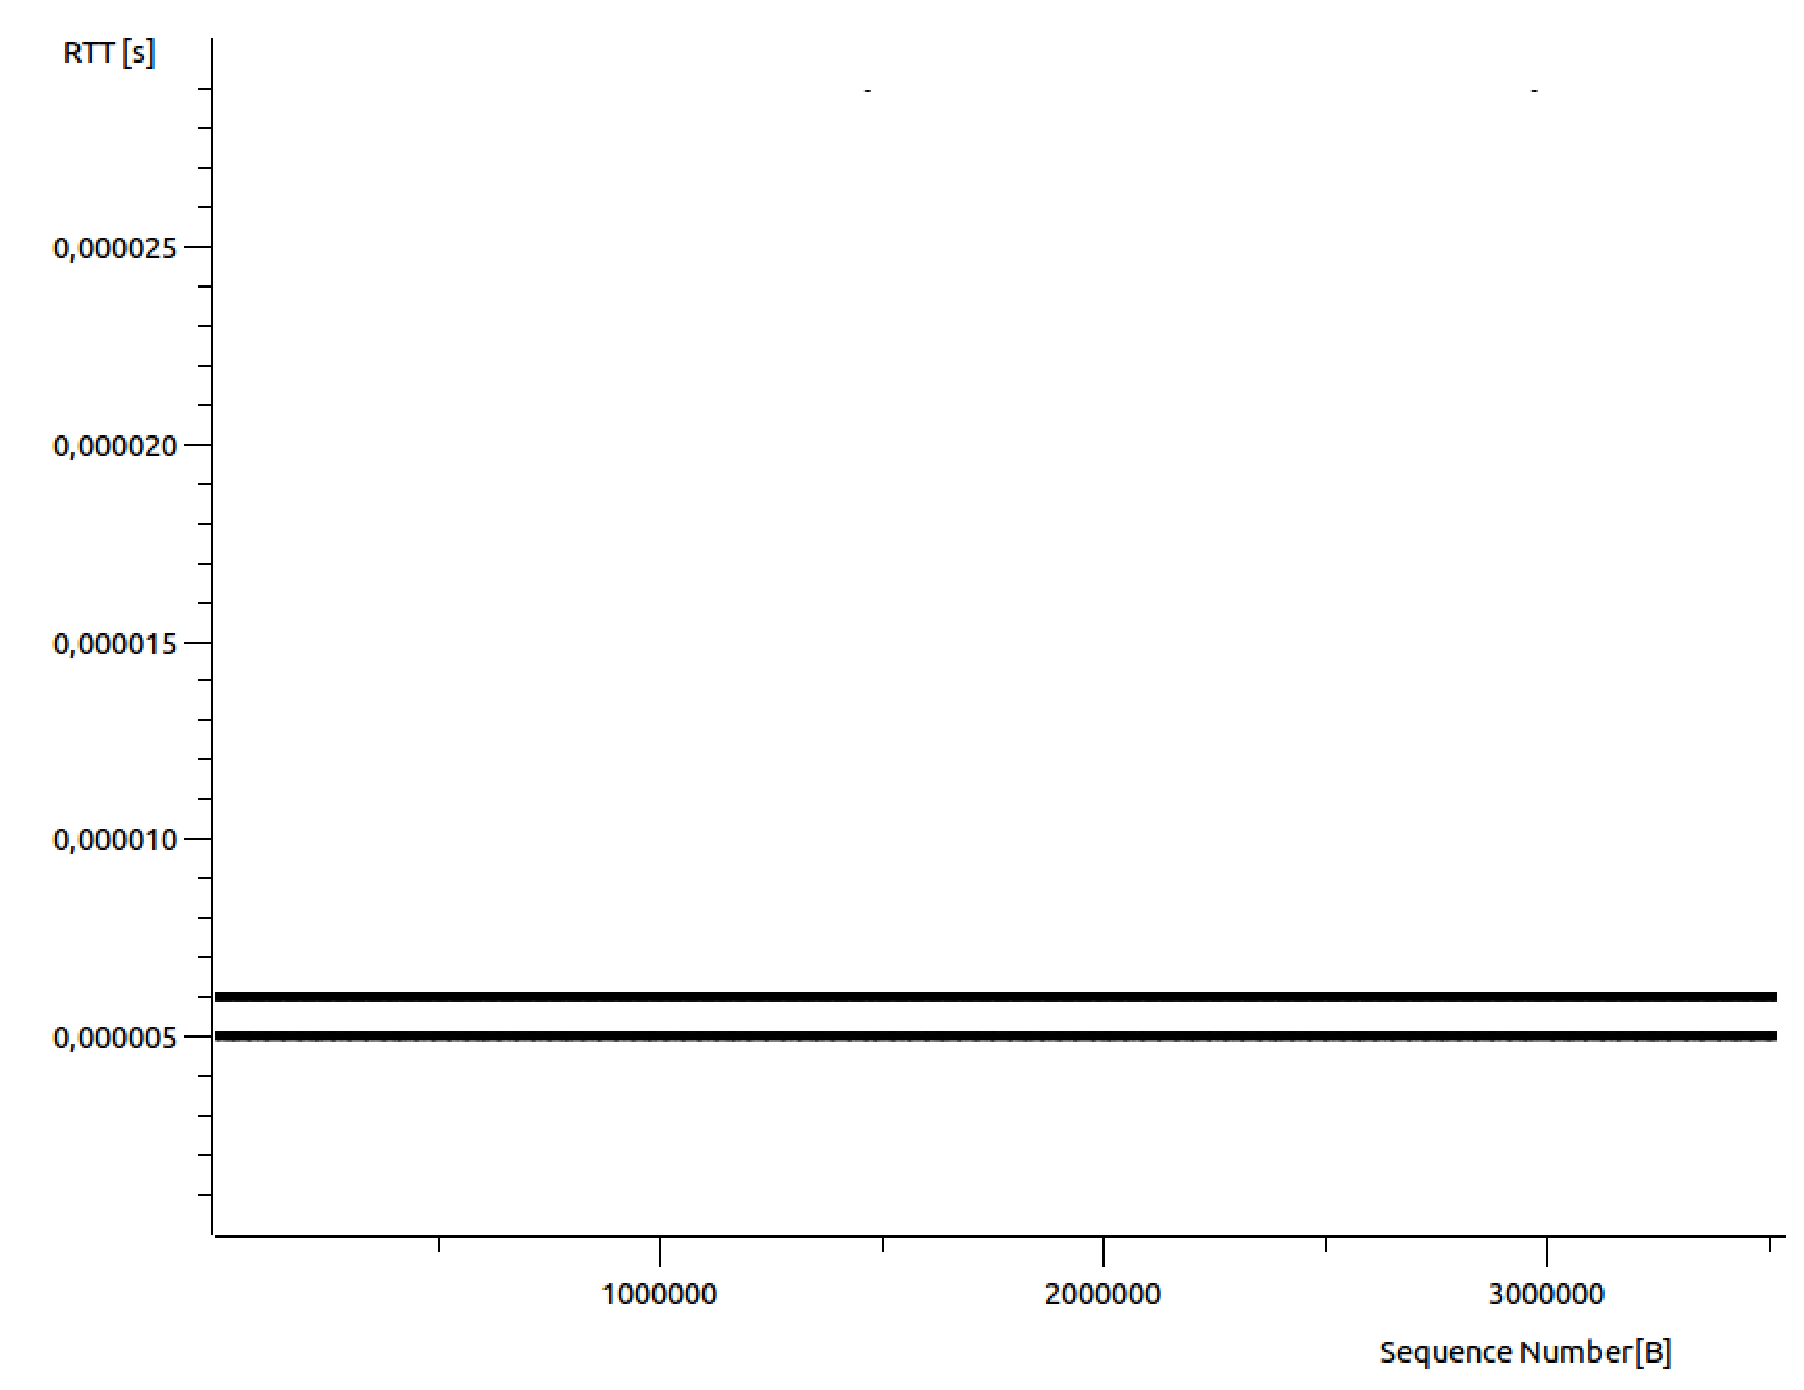
\includegraphics[width=\textwidth]{s1-2_rtt}
  \caption{RTT}
 \end{subfigure}
 \caption{Scene 1-2: TCP Reno + 200 ms delay}
\end{figure}

\begin{figure}
 \centering
 \begin{subfigure}[b]{0.2\textwidth}
  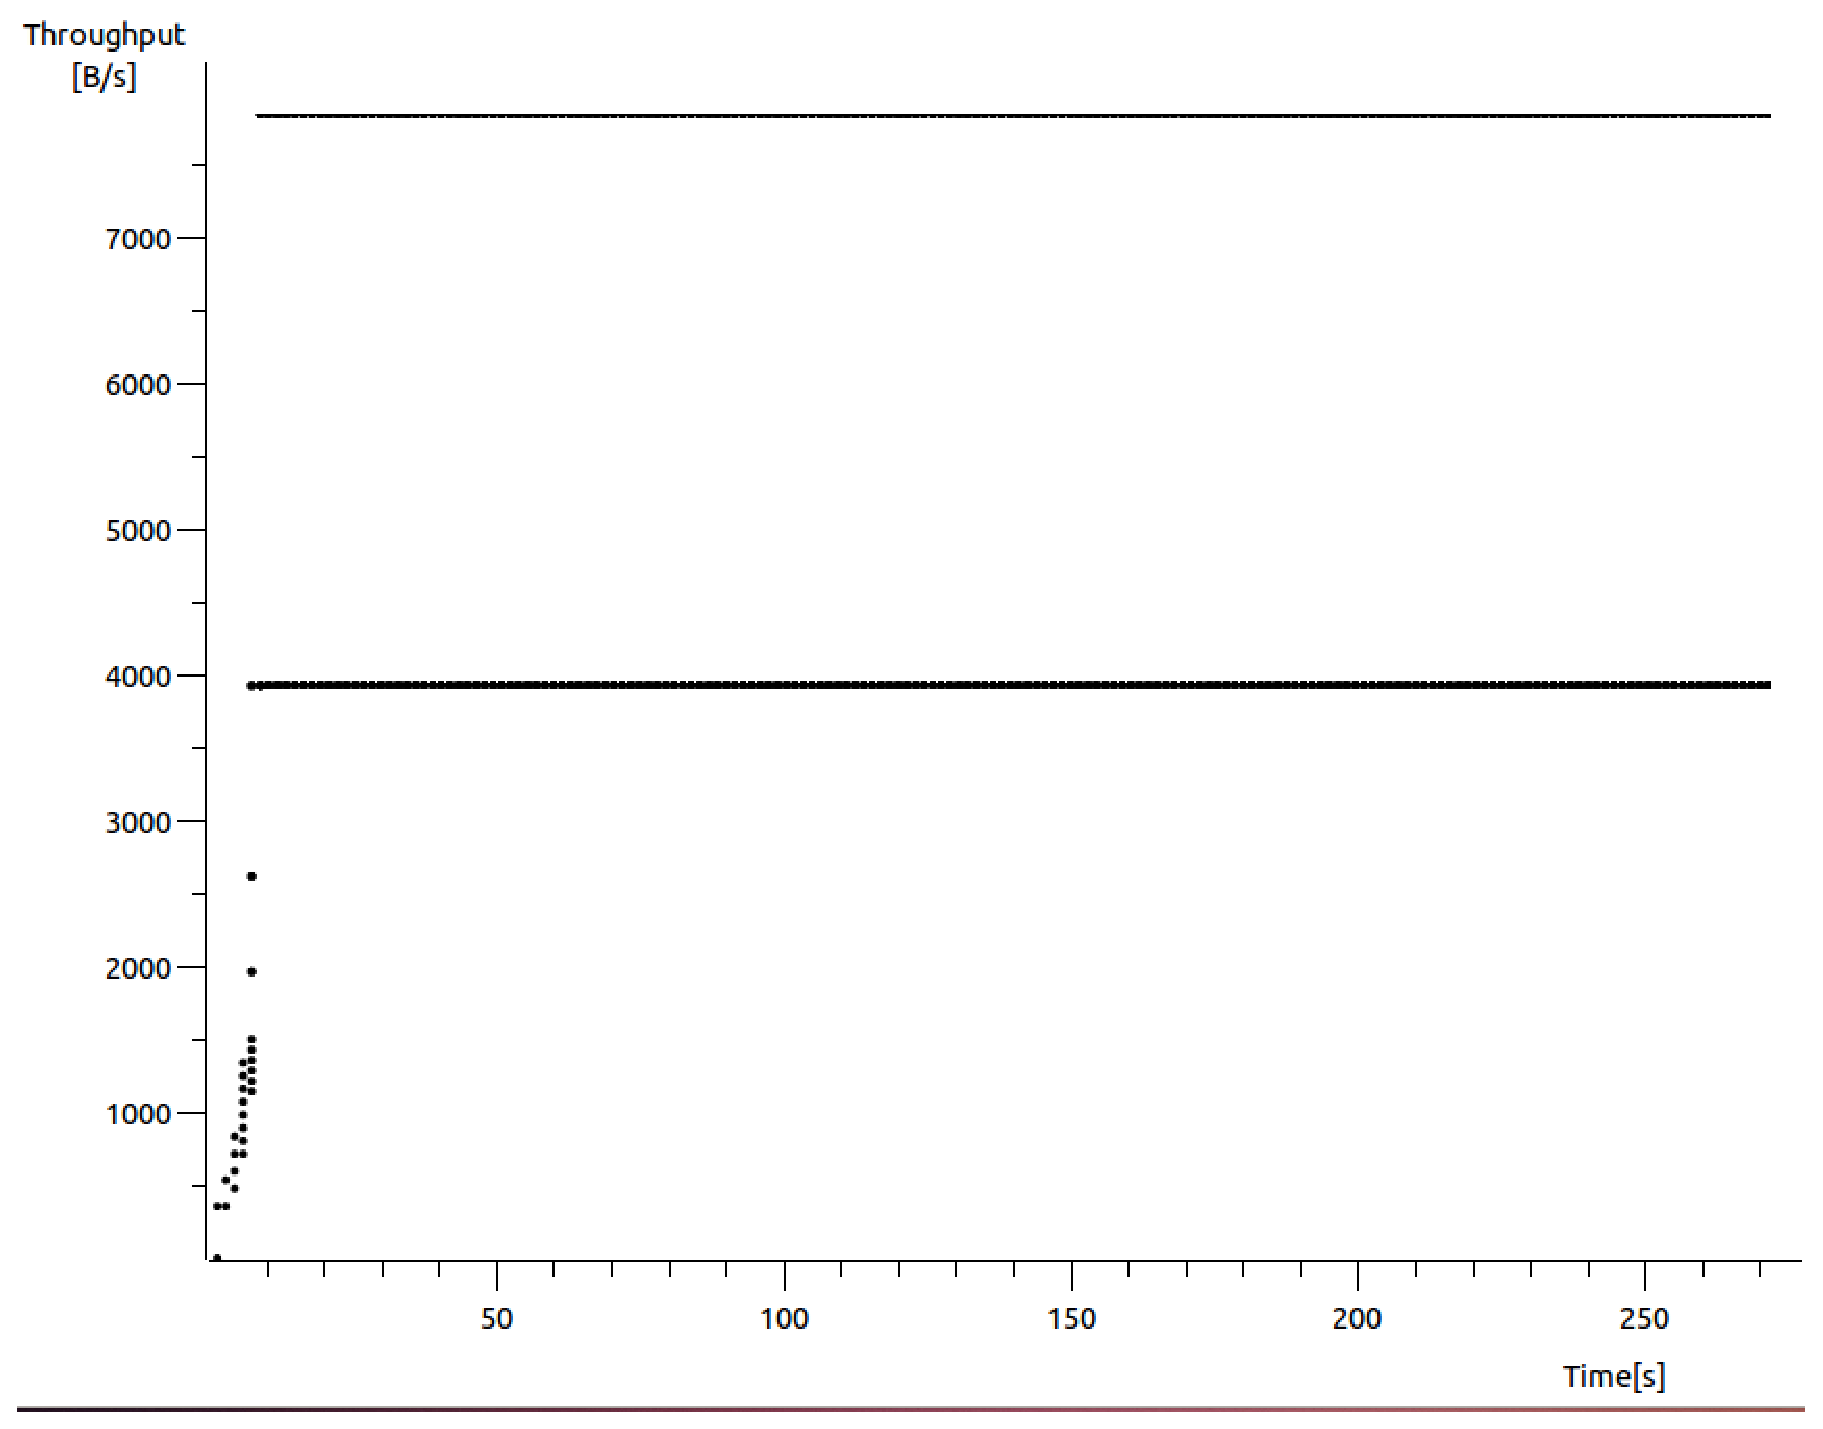
\includegraphics[width=\textwidth]{s1-3_thru}
  \caption{Throughput}
 \end{subfigure}
 \begin{subfigure}[b]{0.2\textwidth}
  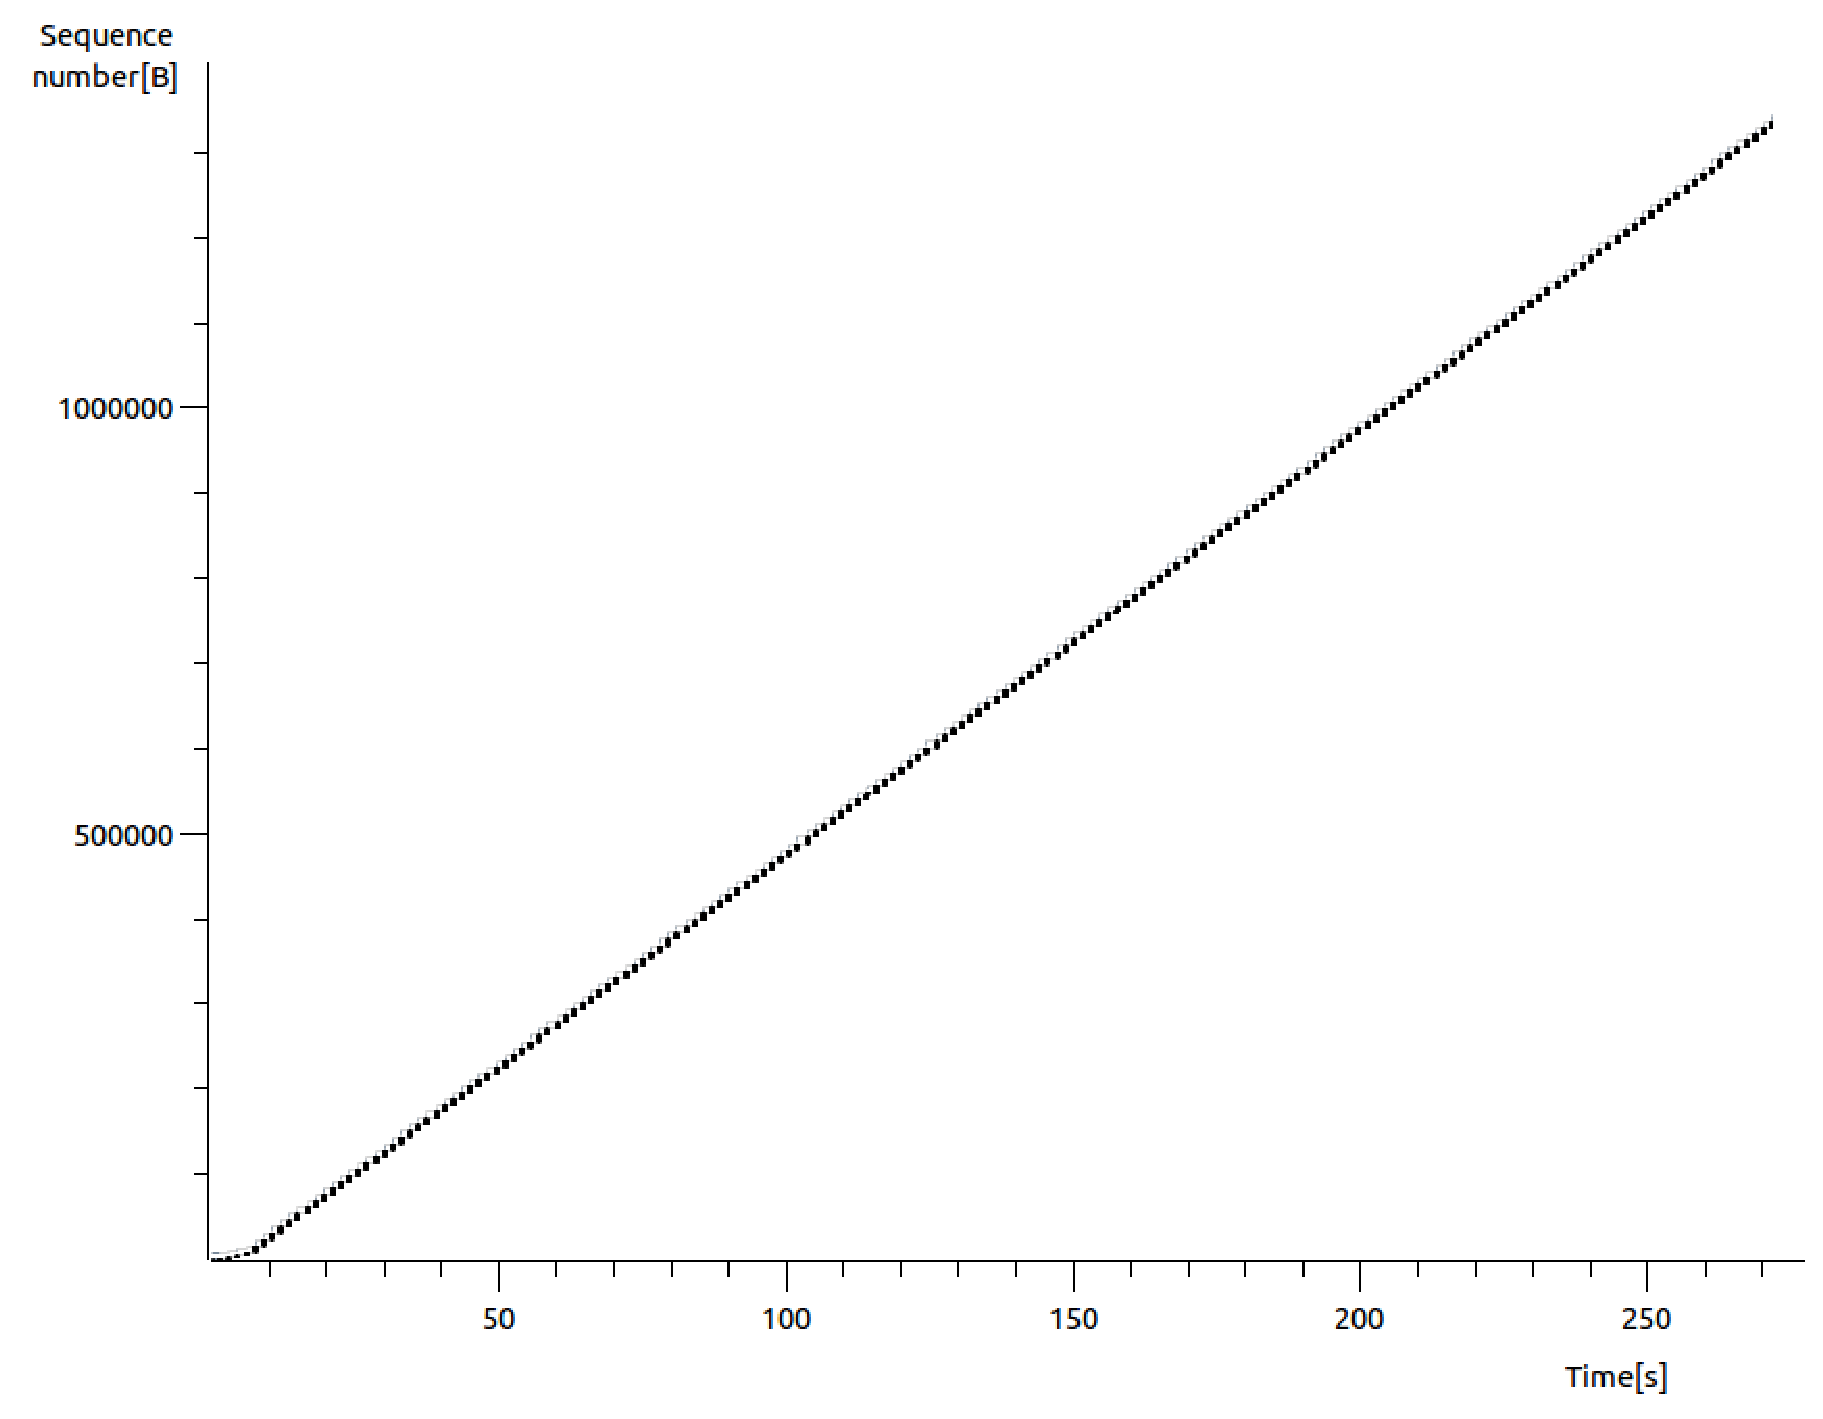
\includegraphics[width=\textwidth]{s1-3_seq}
  \caption{TCP sequence}
 \end{subfigure}
 \begin{subfigure}[b]{0.2\textwidth}
  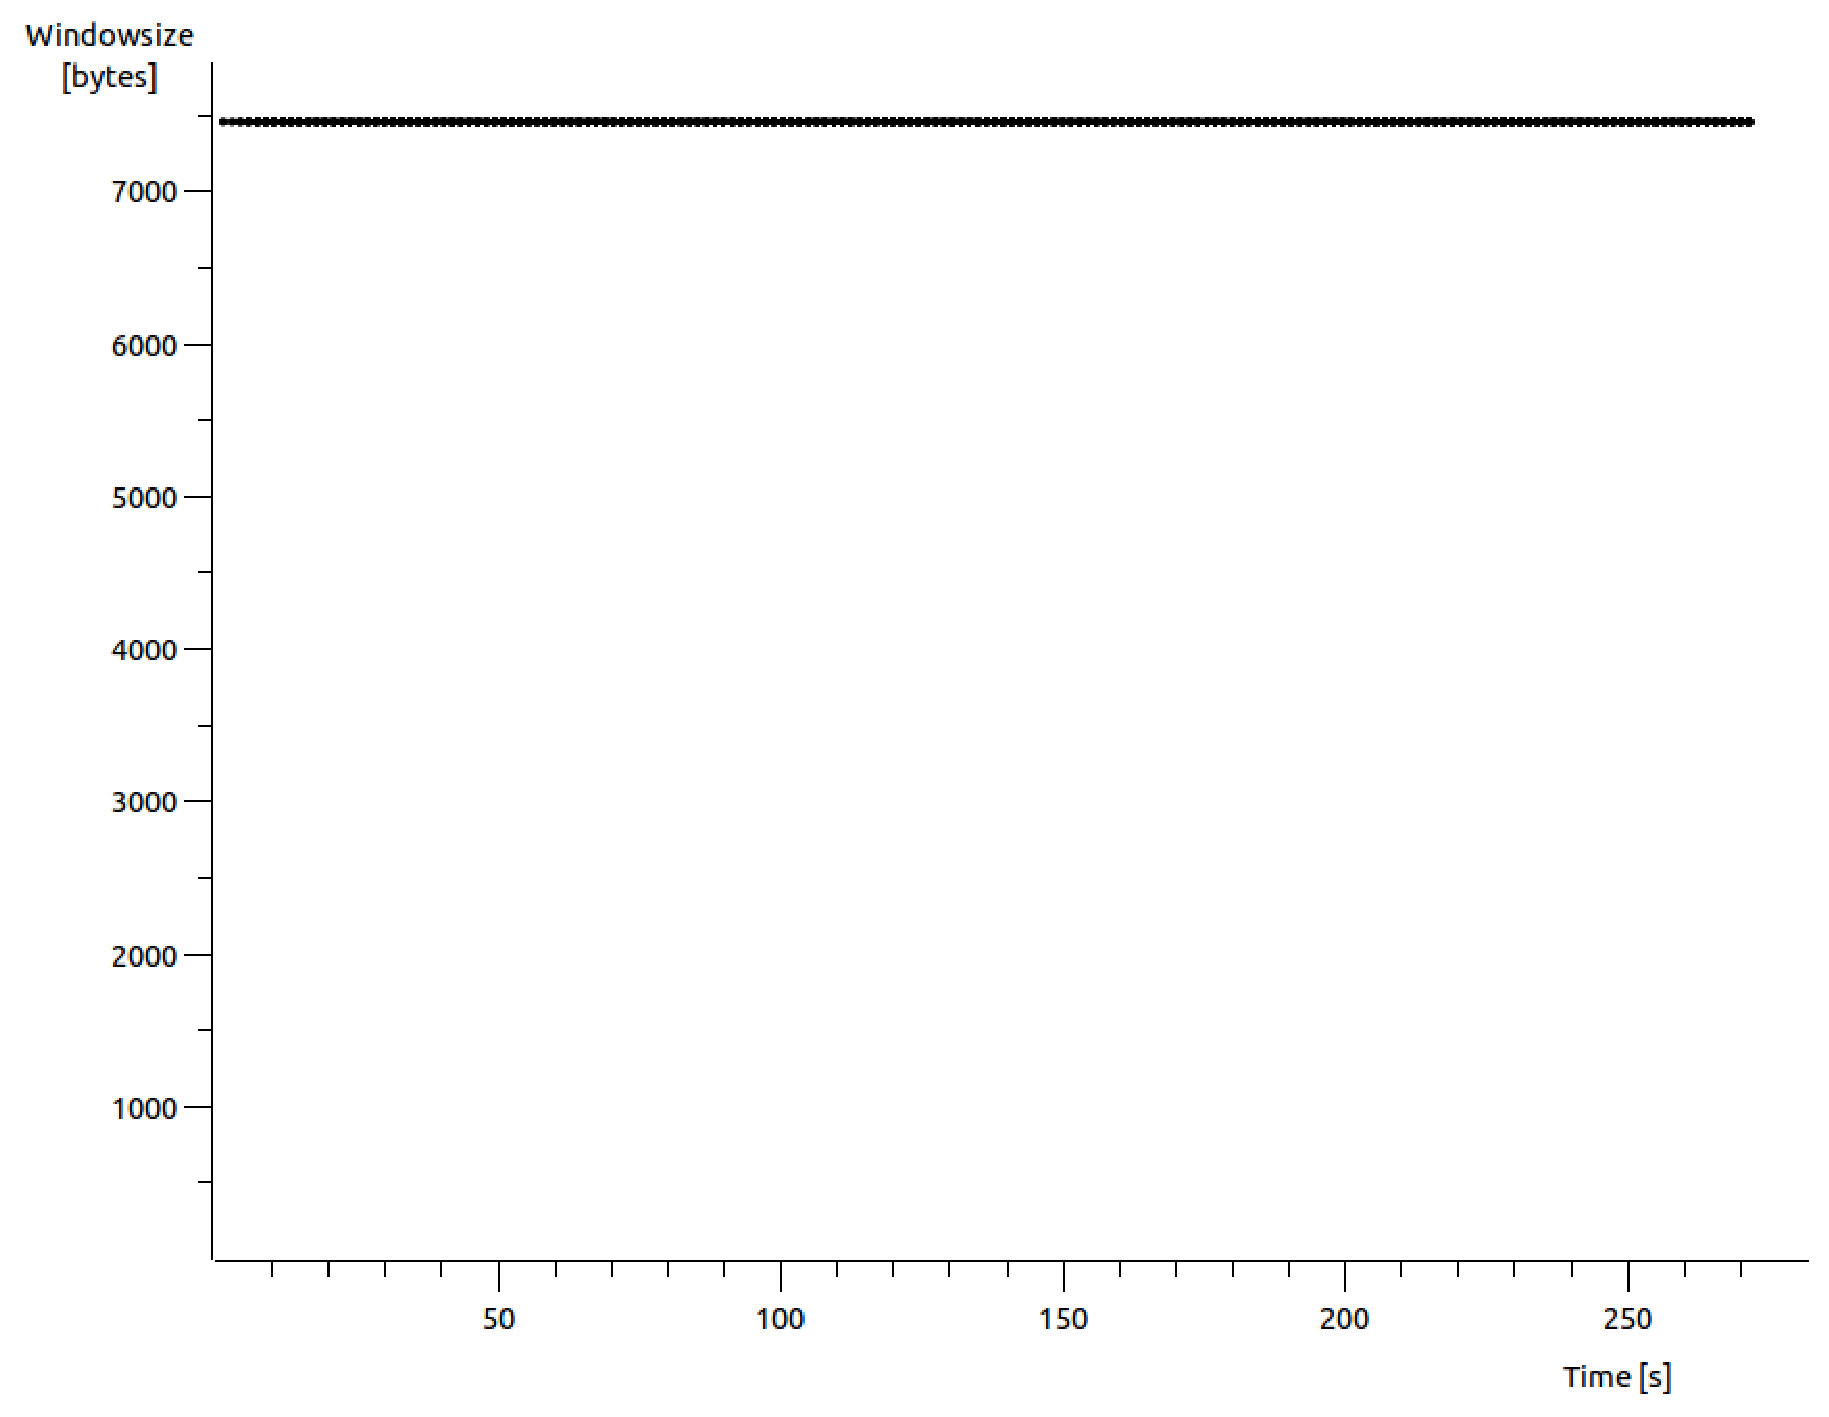
\includegraphics[width=\textwidth]{s1-3_wnd}
  \caption{Window size}
 \end{subfigure}
 \begin{subfigure}[b]{0.2\textwidth}
  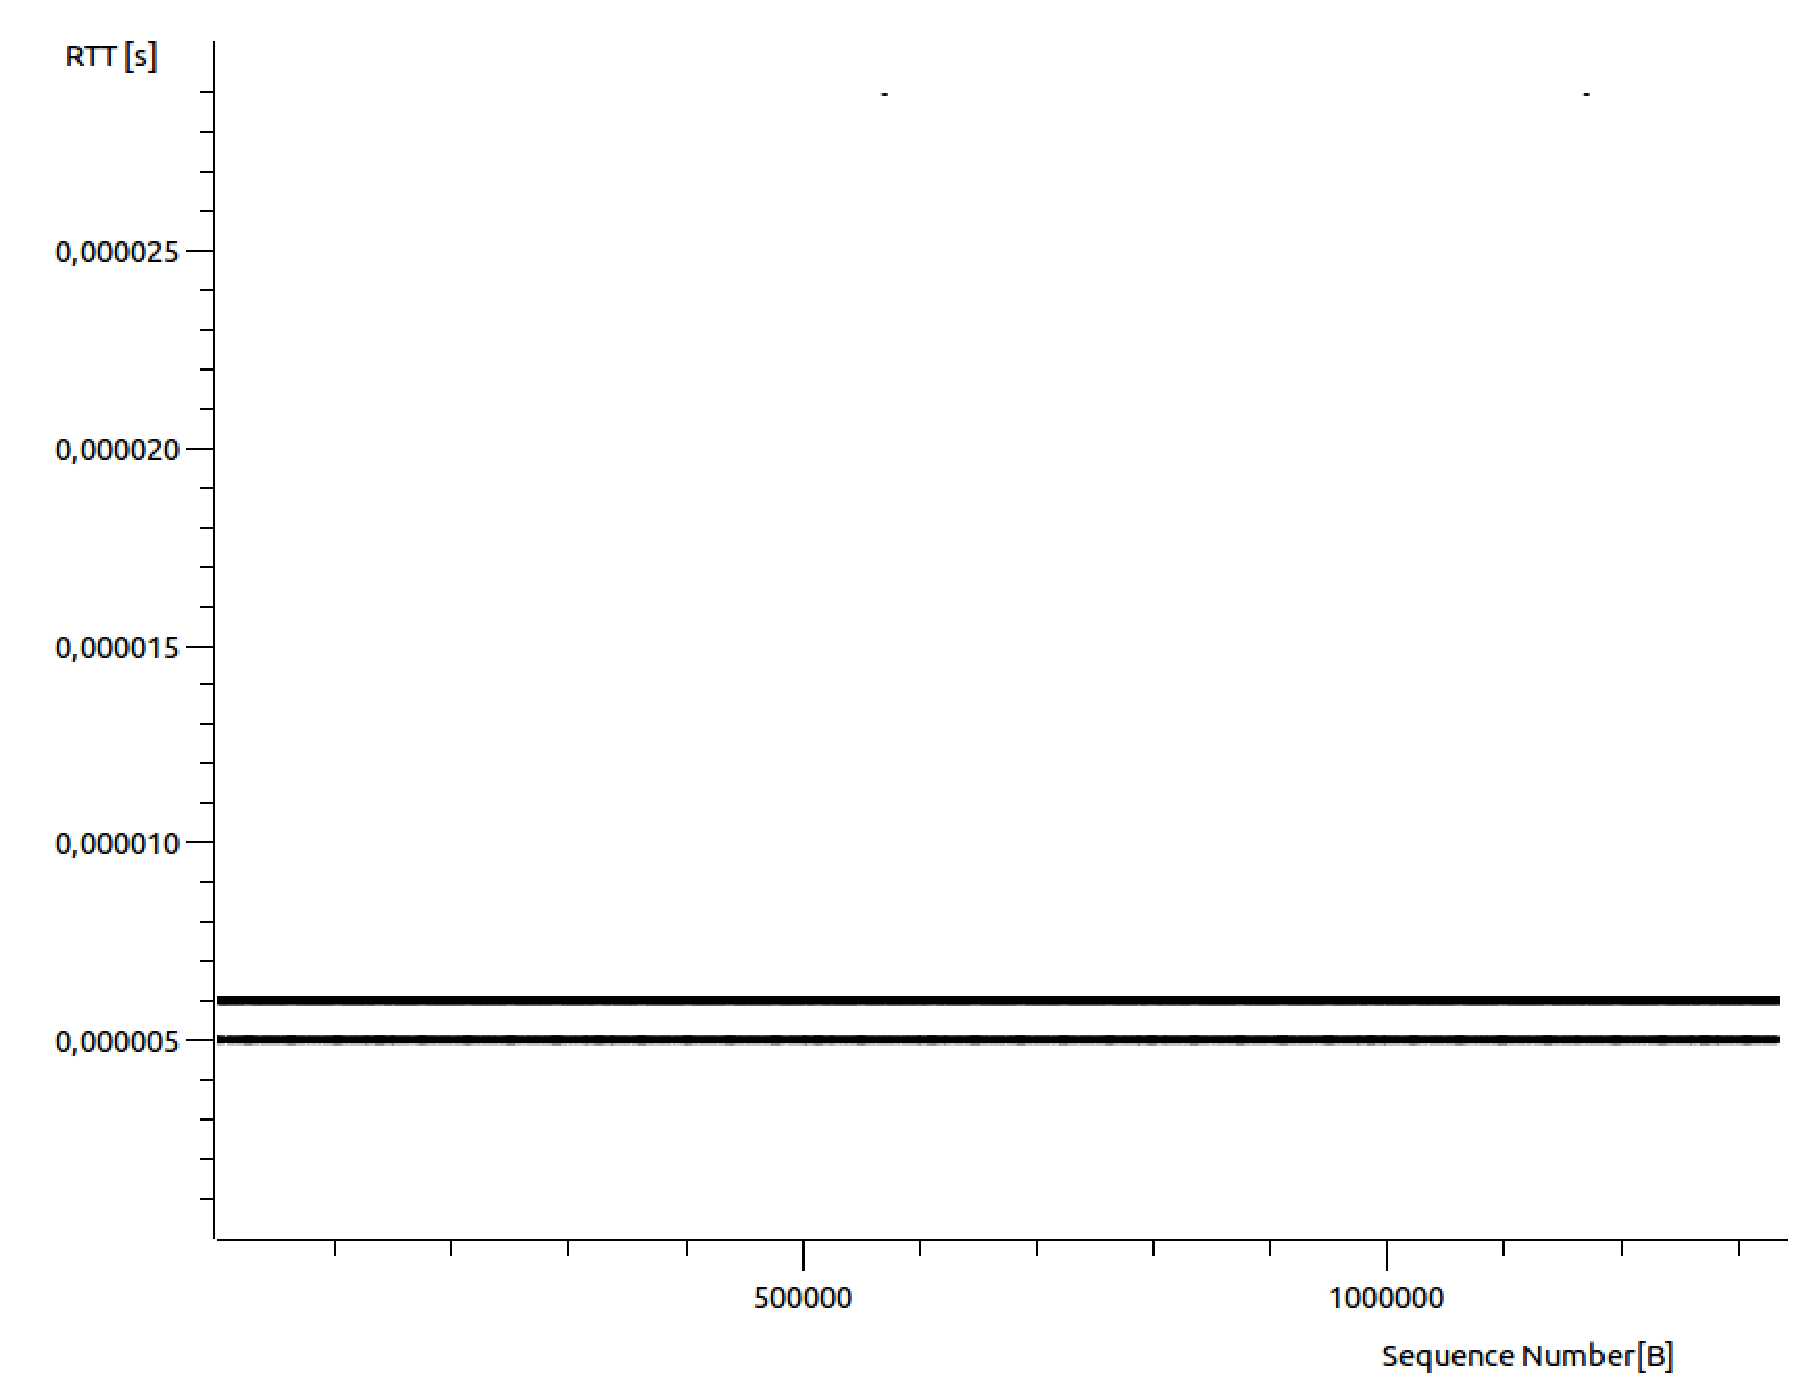
\includegraphics[width=\textwidth]{s1-3_rtt}
  \caption{RTT}
 \end{subfigure}
 \caption{Scene 1-3: TCP Reno + 250 delay}
\end{figure}

\begin{figure}
 \centering
 \begin{subfigure}[b]{0.2\textwidth}
  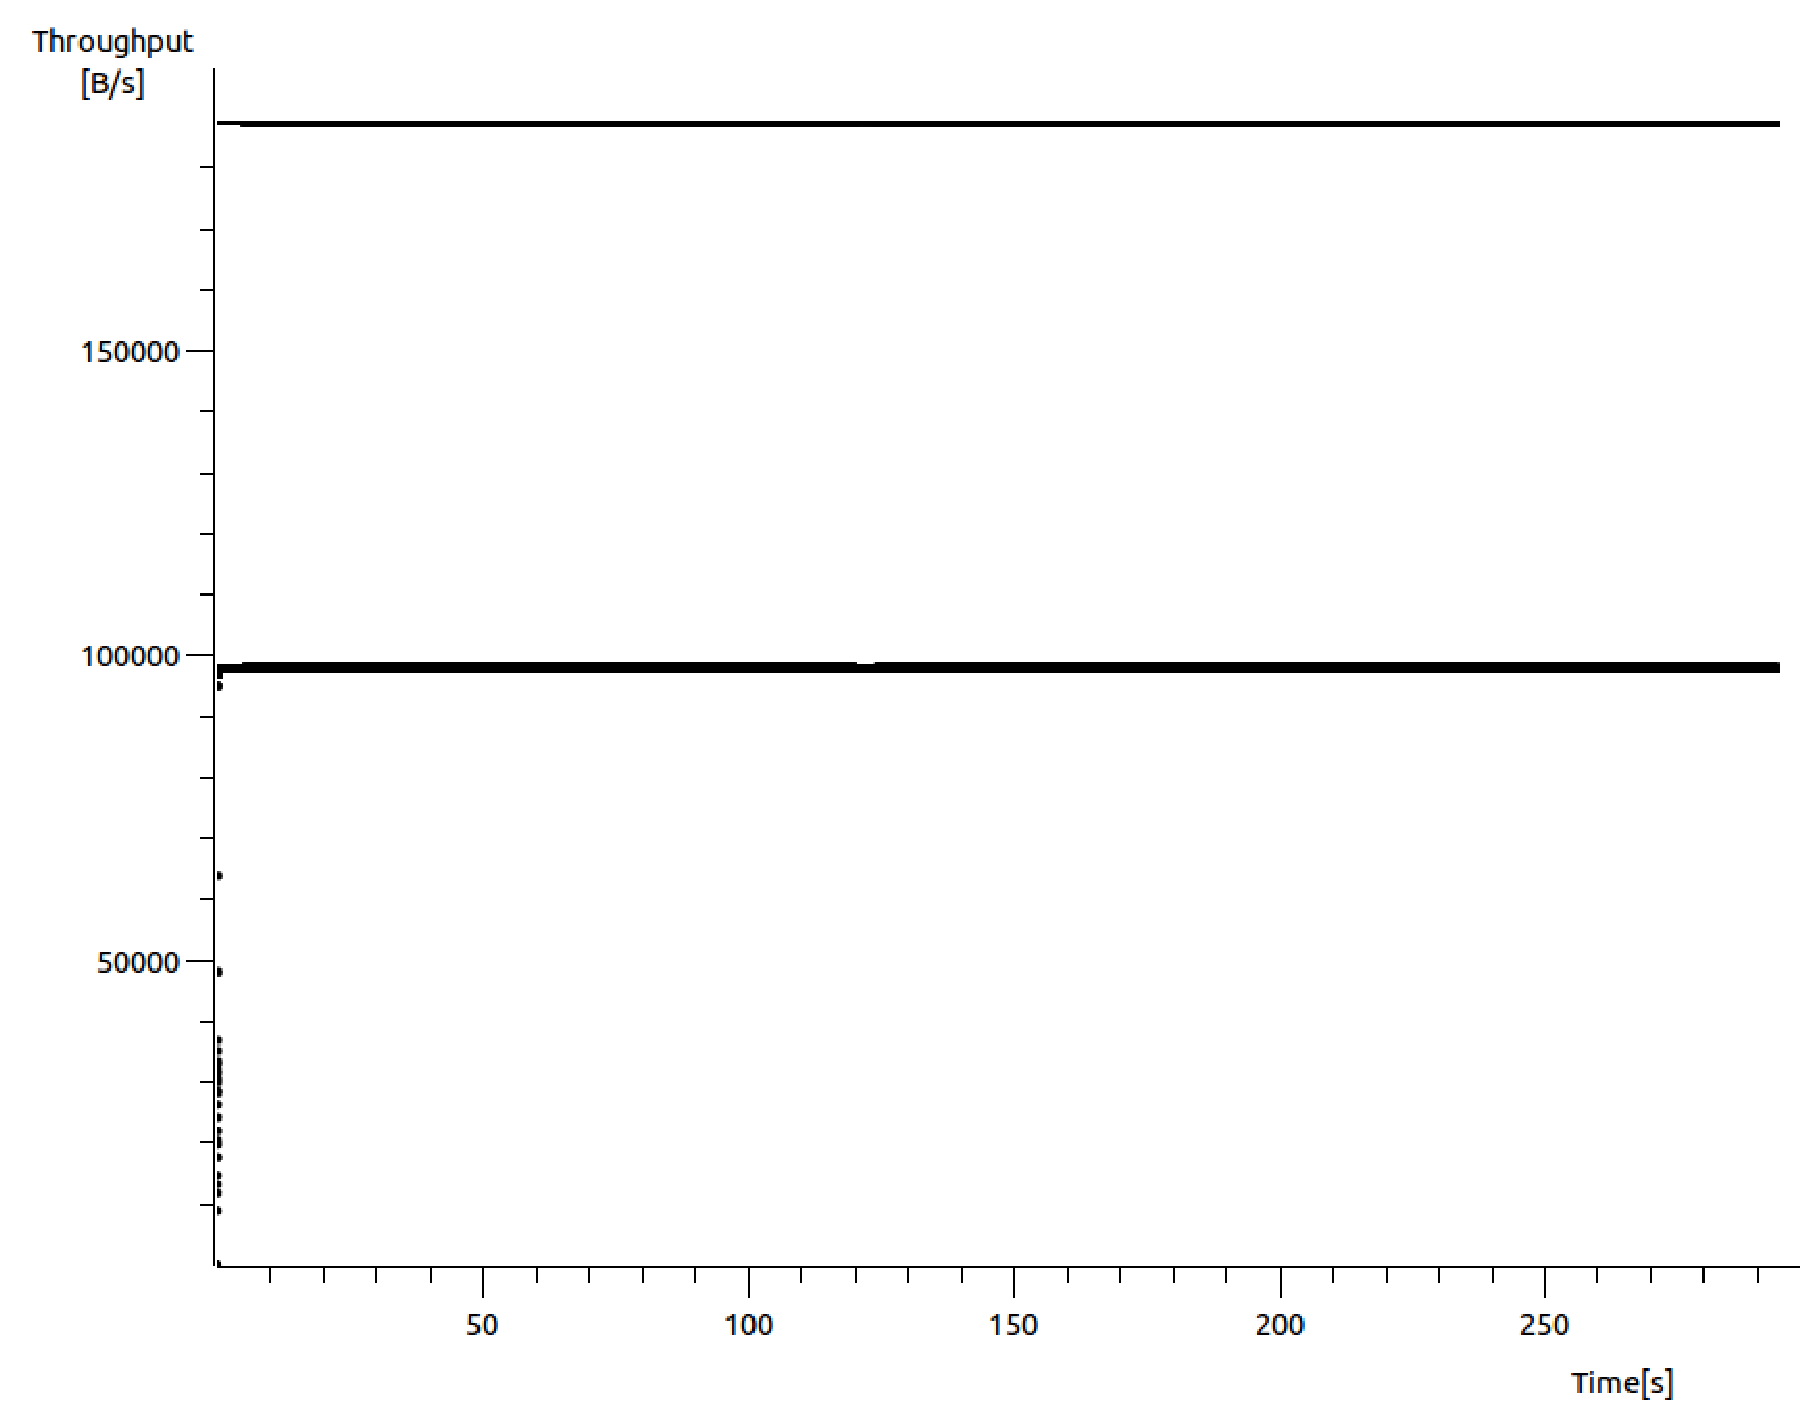
\includegraphics[width=\textwidth]{s4-0_thru}
  \caption{Throughput}
 \end{subfigure}
 \begin{subfigure}[b]{0.2\textwidth}
  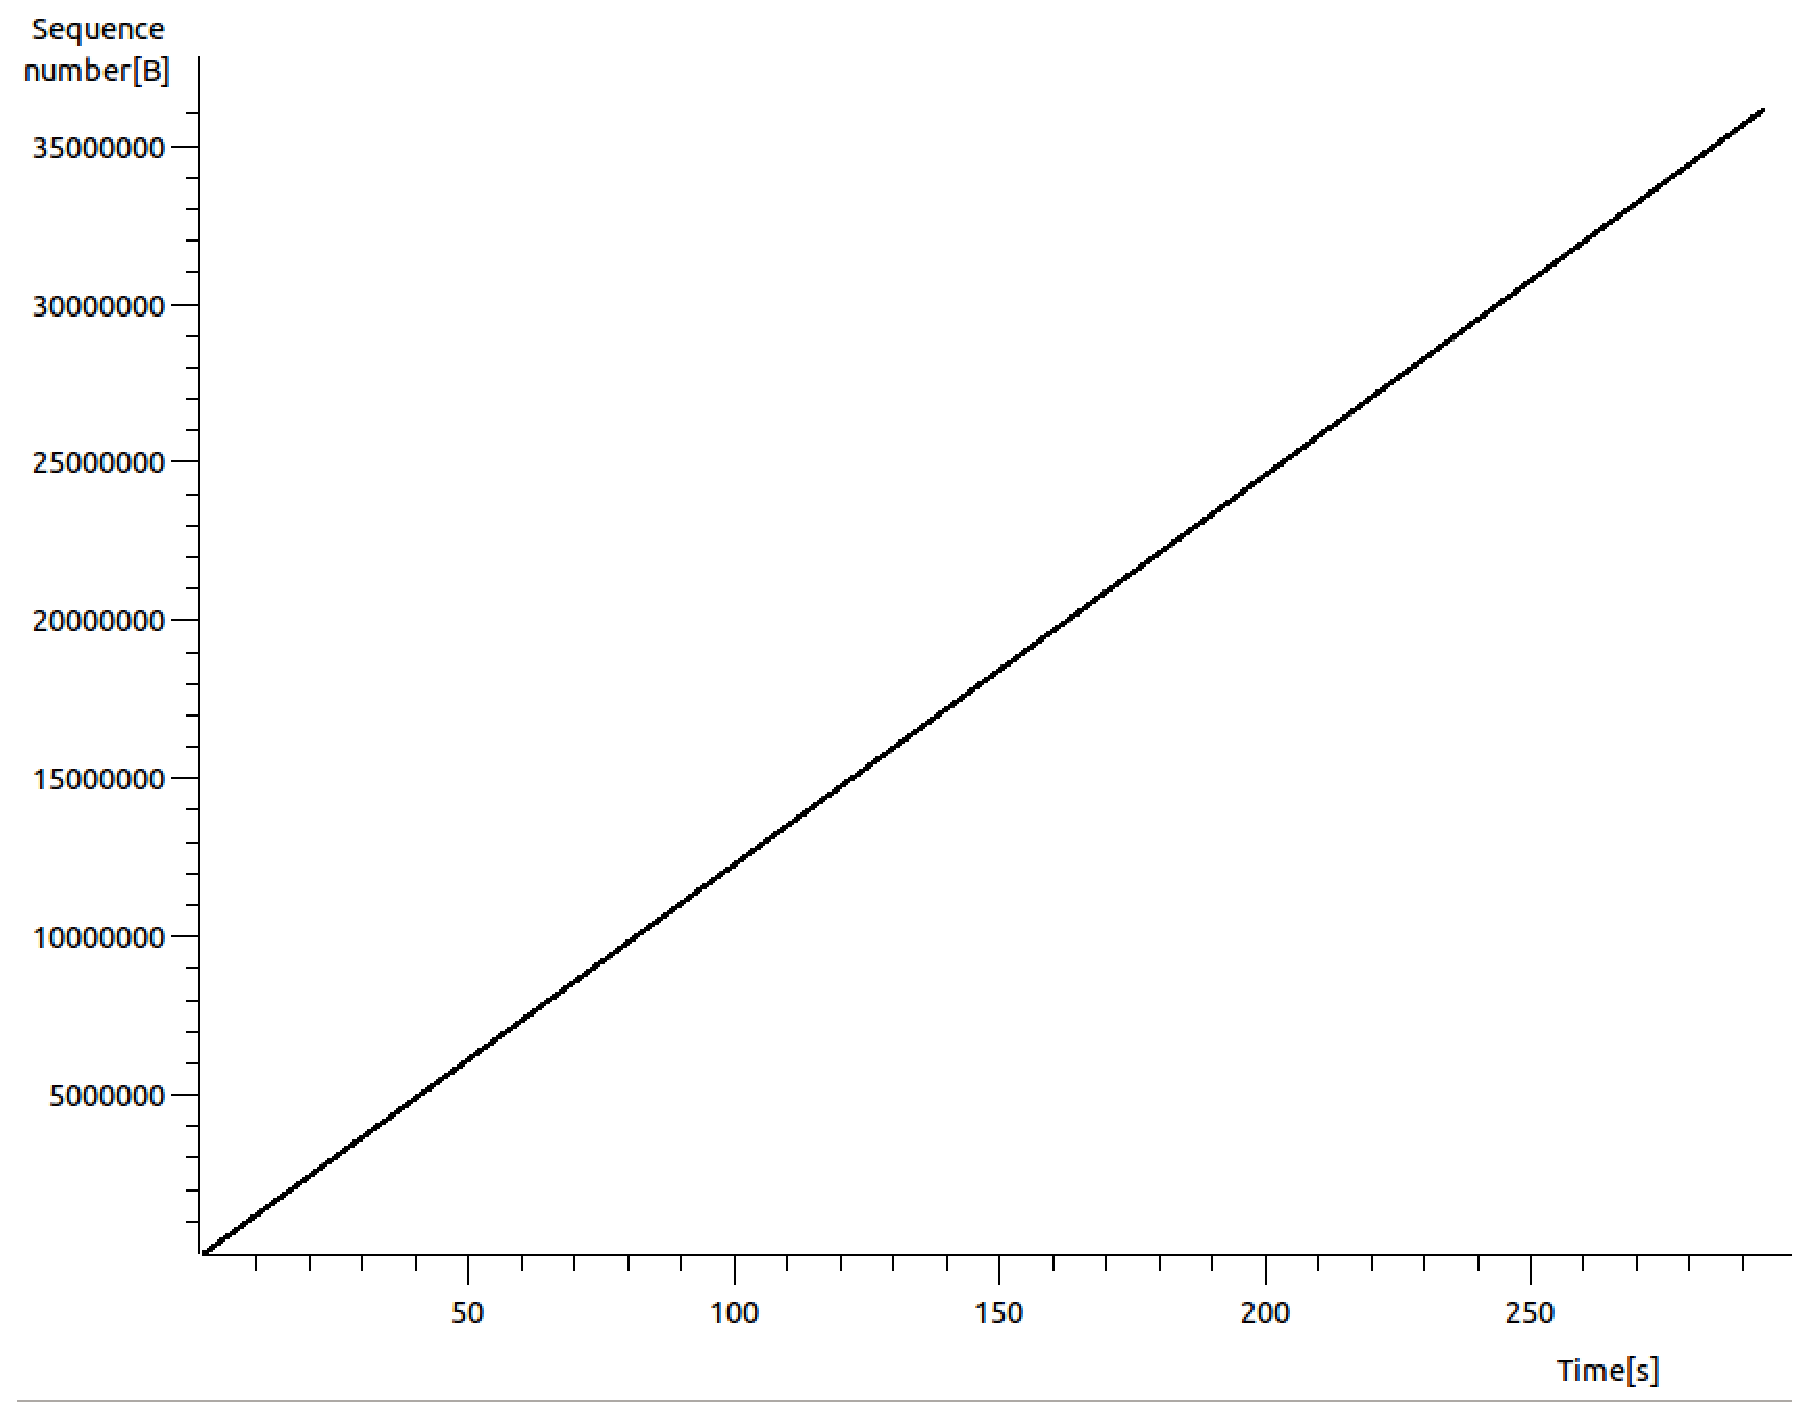
\includegraphics[width=\textwidth]{s4-0_seq}
  \caption{TCP sequence}
 \end{subfigure}
 \begin{subfigure}[b]{0.2\textwidth}
  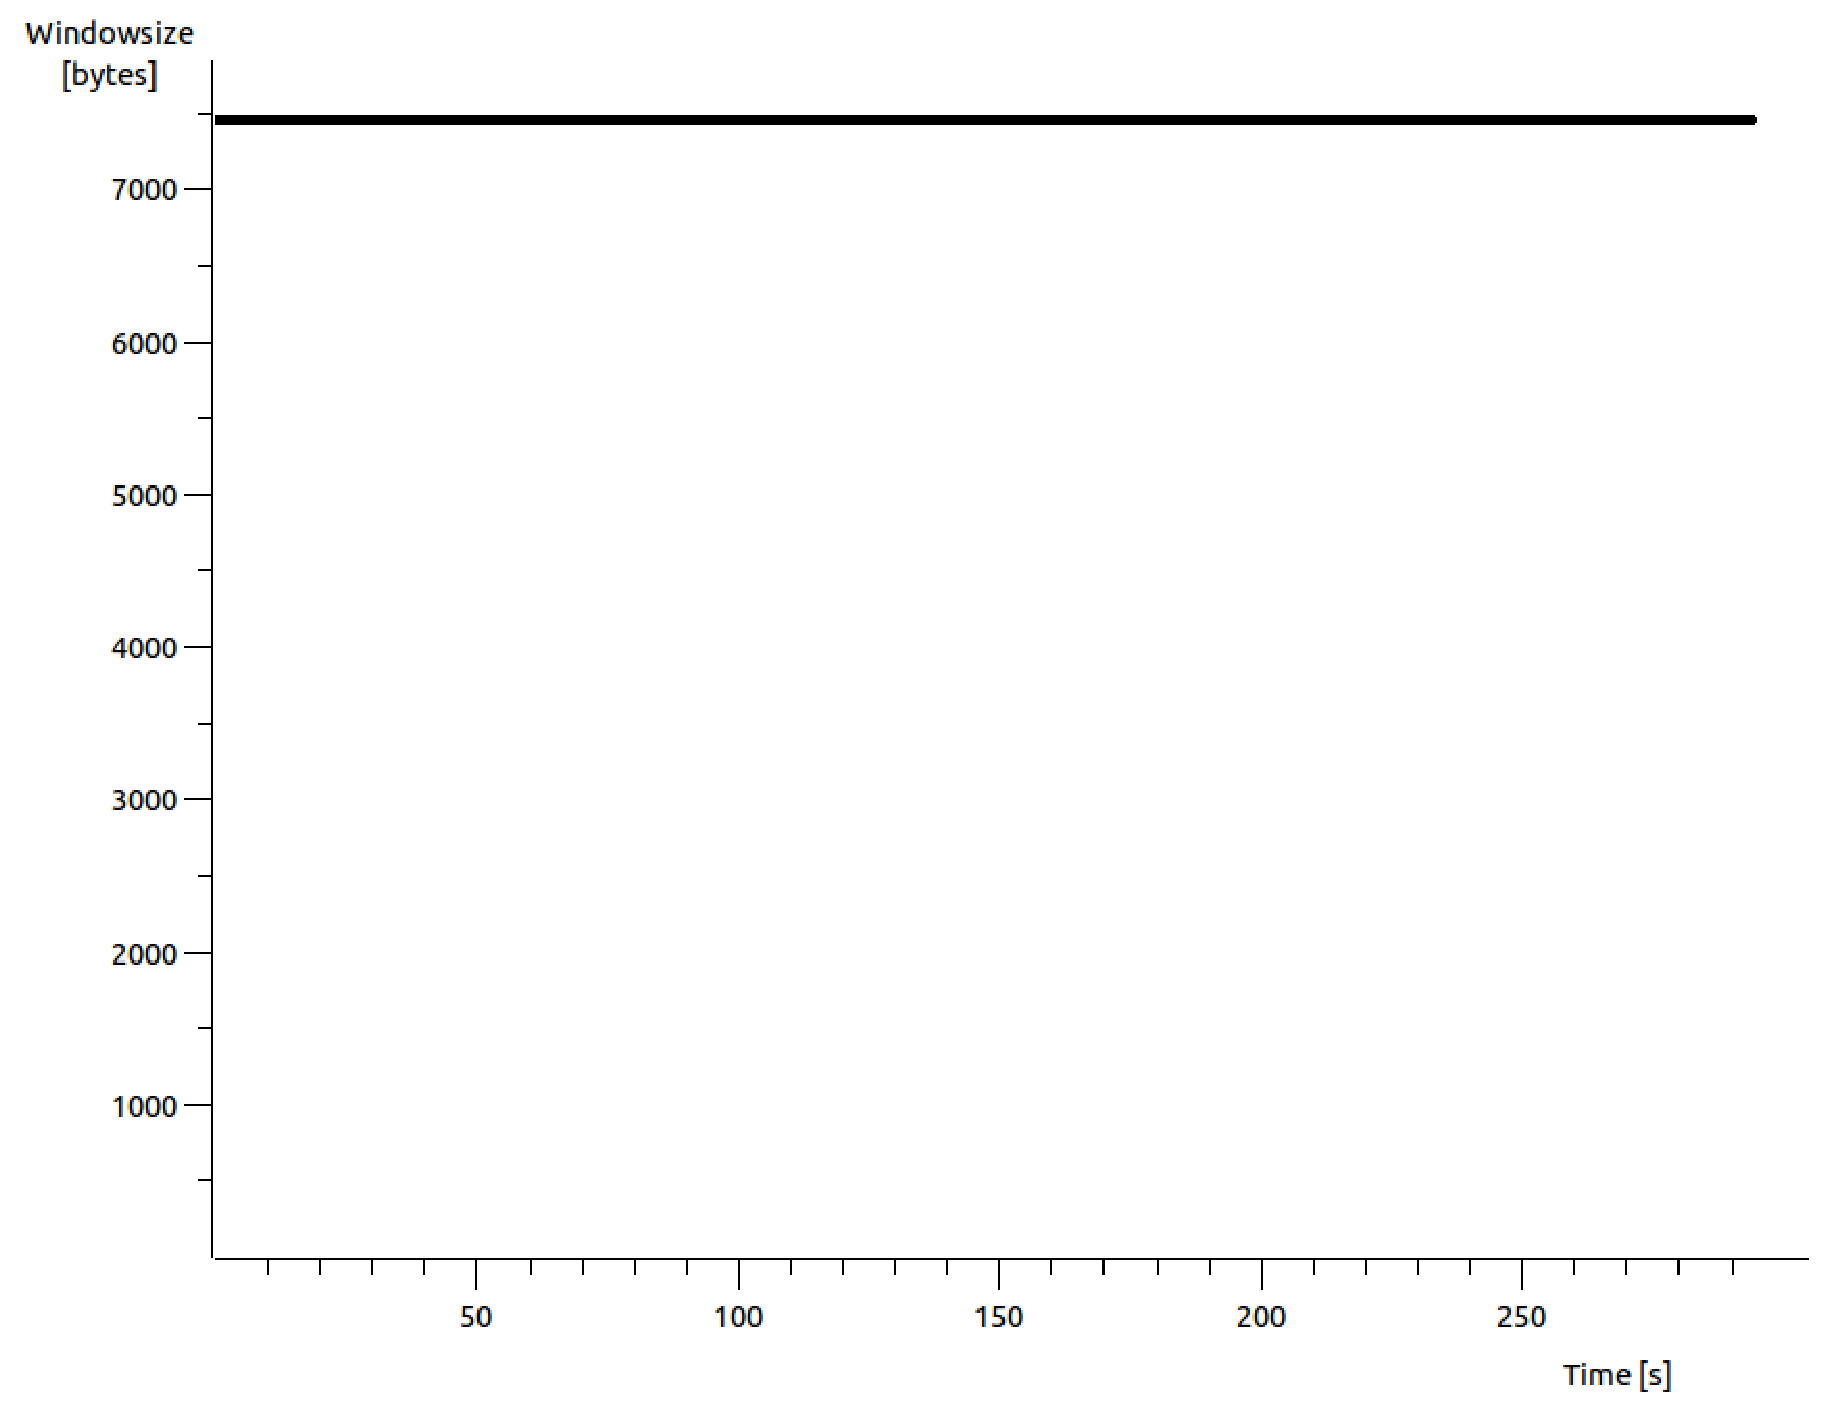
\includegraphics[width=\textwidth]{s4-0_wnd}
  \caption{Window size}
 \end{subfigure}
 \begin{subfigure}[b]{0.2\textwidth}
  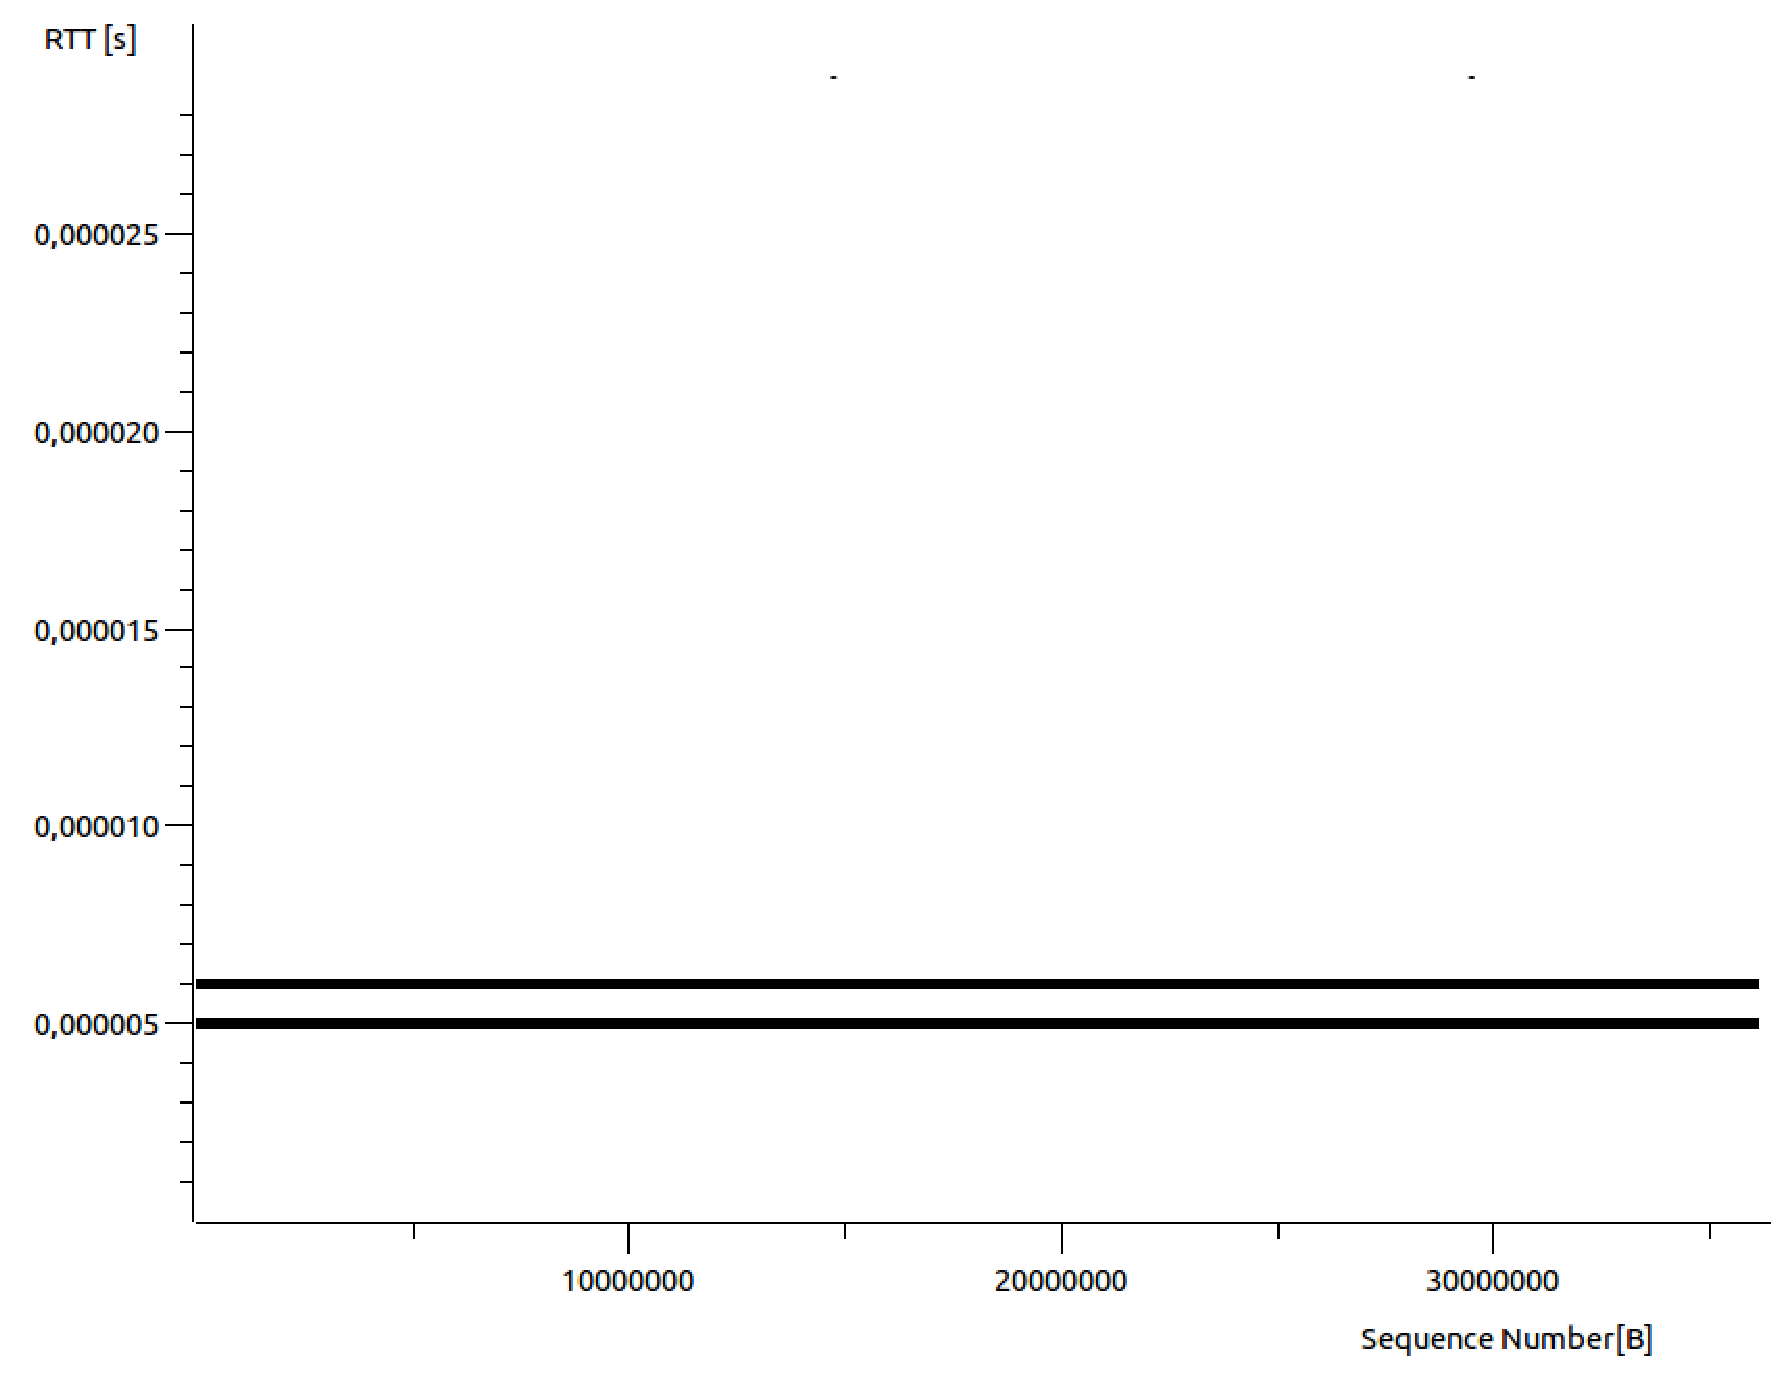
\includegraphics[width=\textwidth]{s4-0_rtt}
  \caption{RTT}
 \end{subfigure}
 \caption{Scene 4-0: TCP New Reno + 10 ms delay}
\end{figure}

\begin{figure}
 \centering
 \begin{subfigure}[b]{0.2\textwidth}
  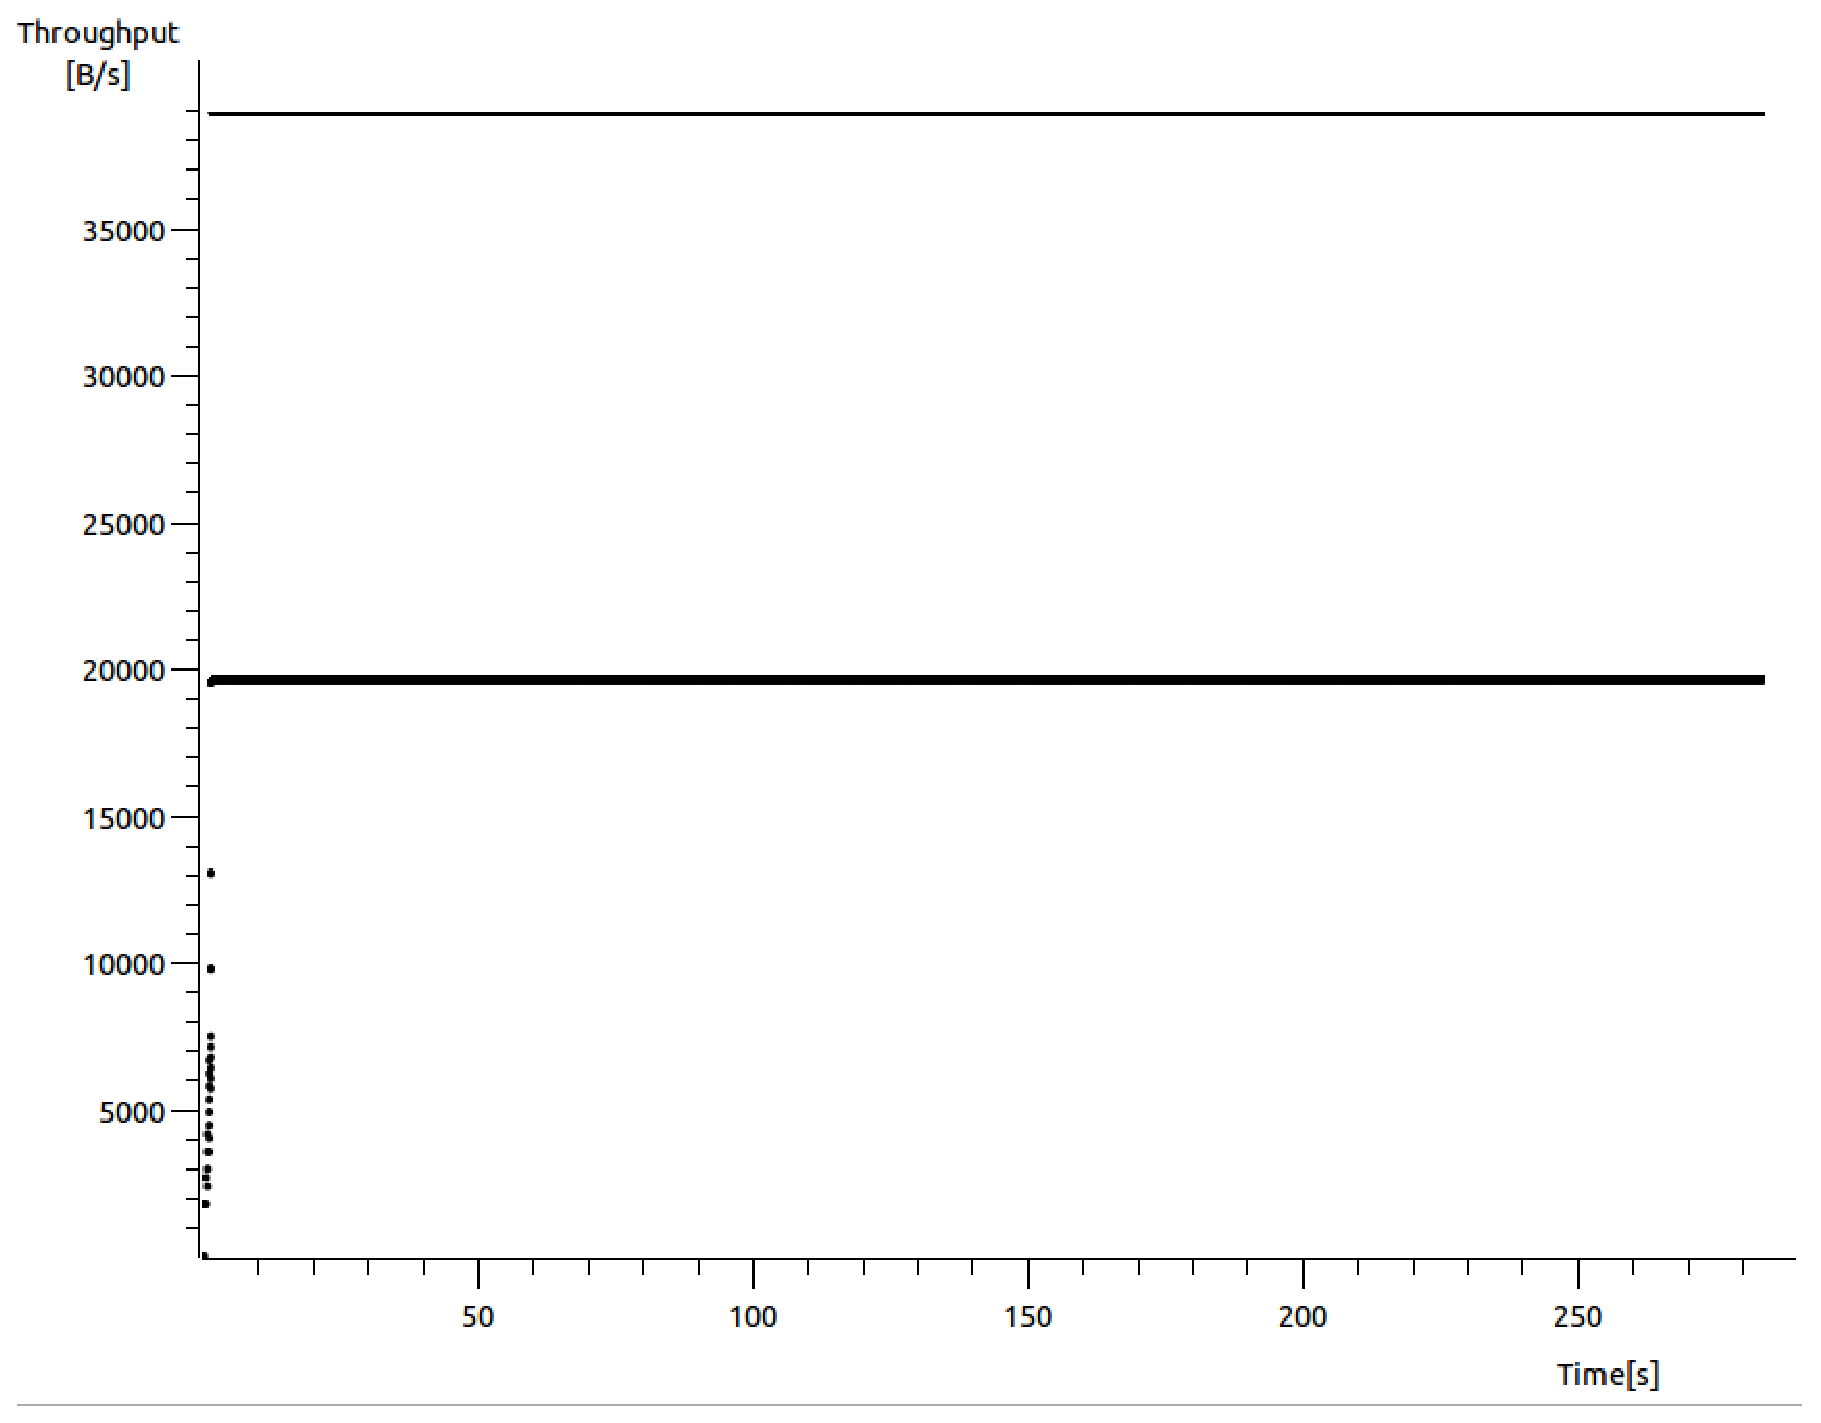
\includegraphics[width=\textwidth]{s4-1_thru}
  \caption{Throughput}
 \end{subfigure}
 \begin{subfigure}[b]{0.2\textwidth}
  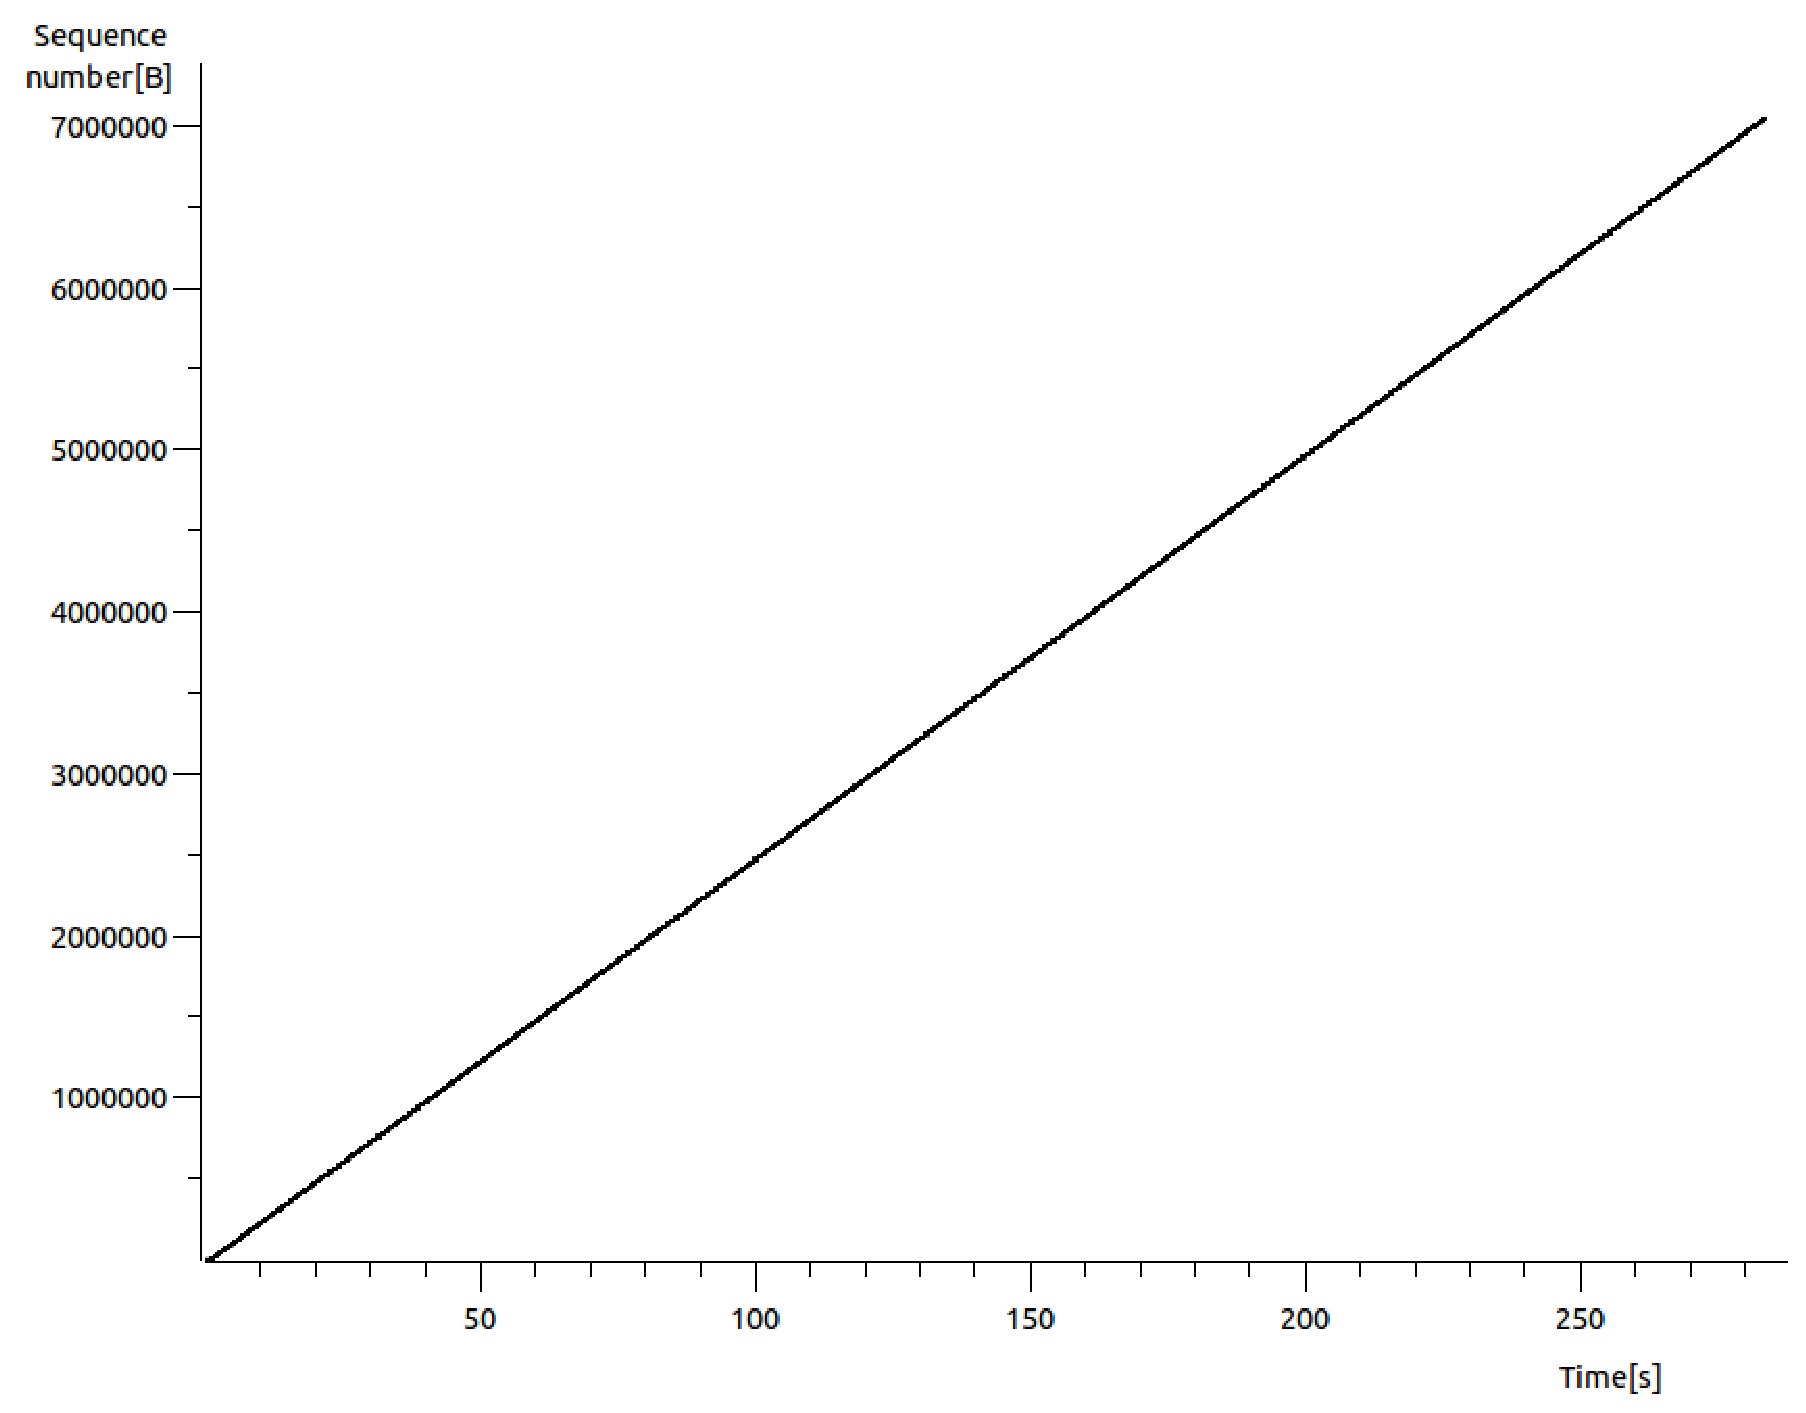
\includegraphics[width=\textwidth]{s4-1_seq}
  \caption{TCP sequence}
 \end{subfigure}
 \begin{subfigure}[b]{0.2\textwidth}
  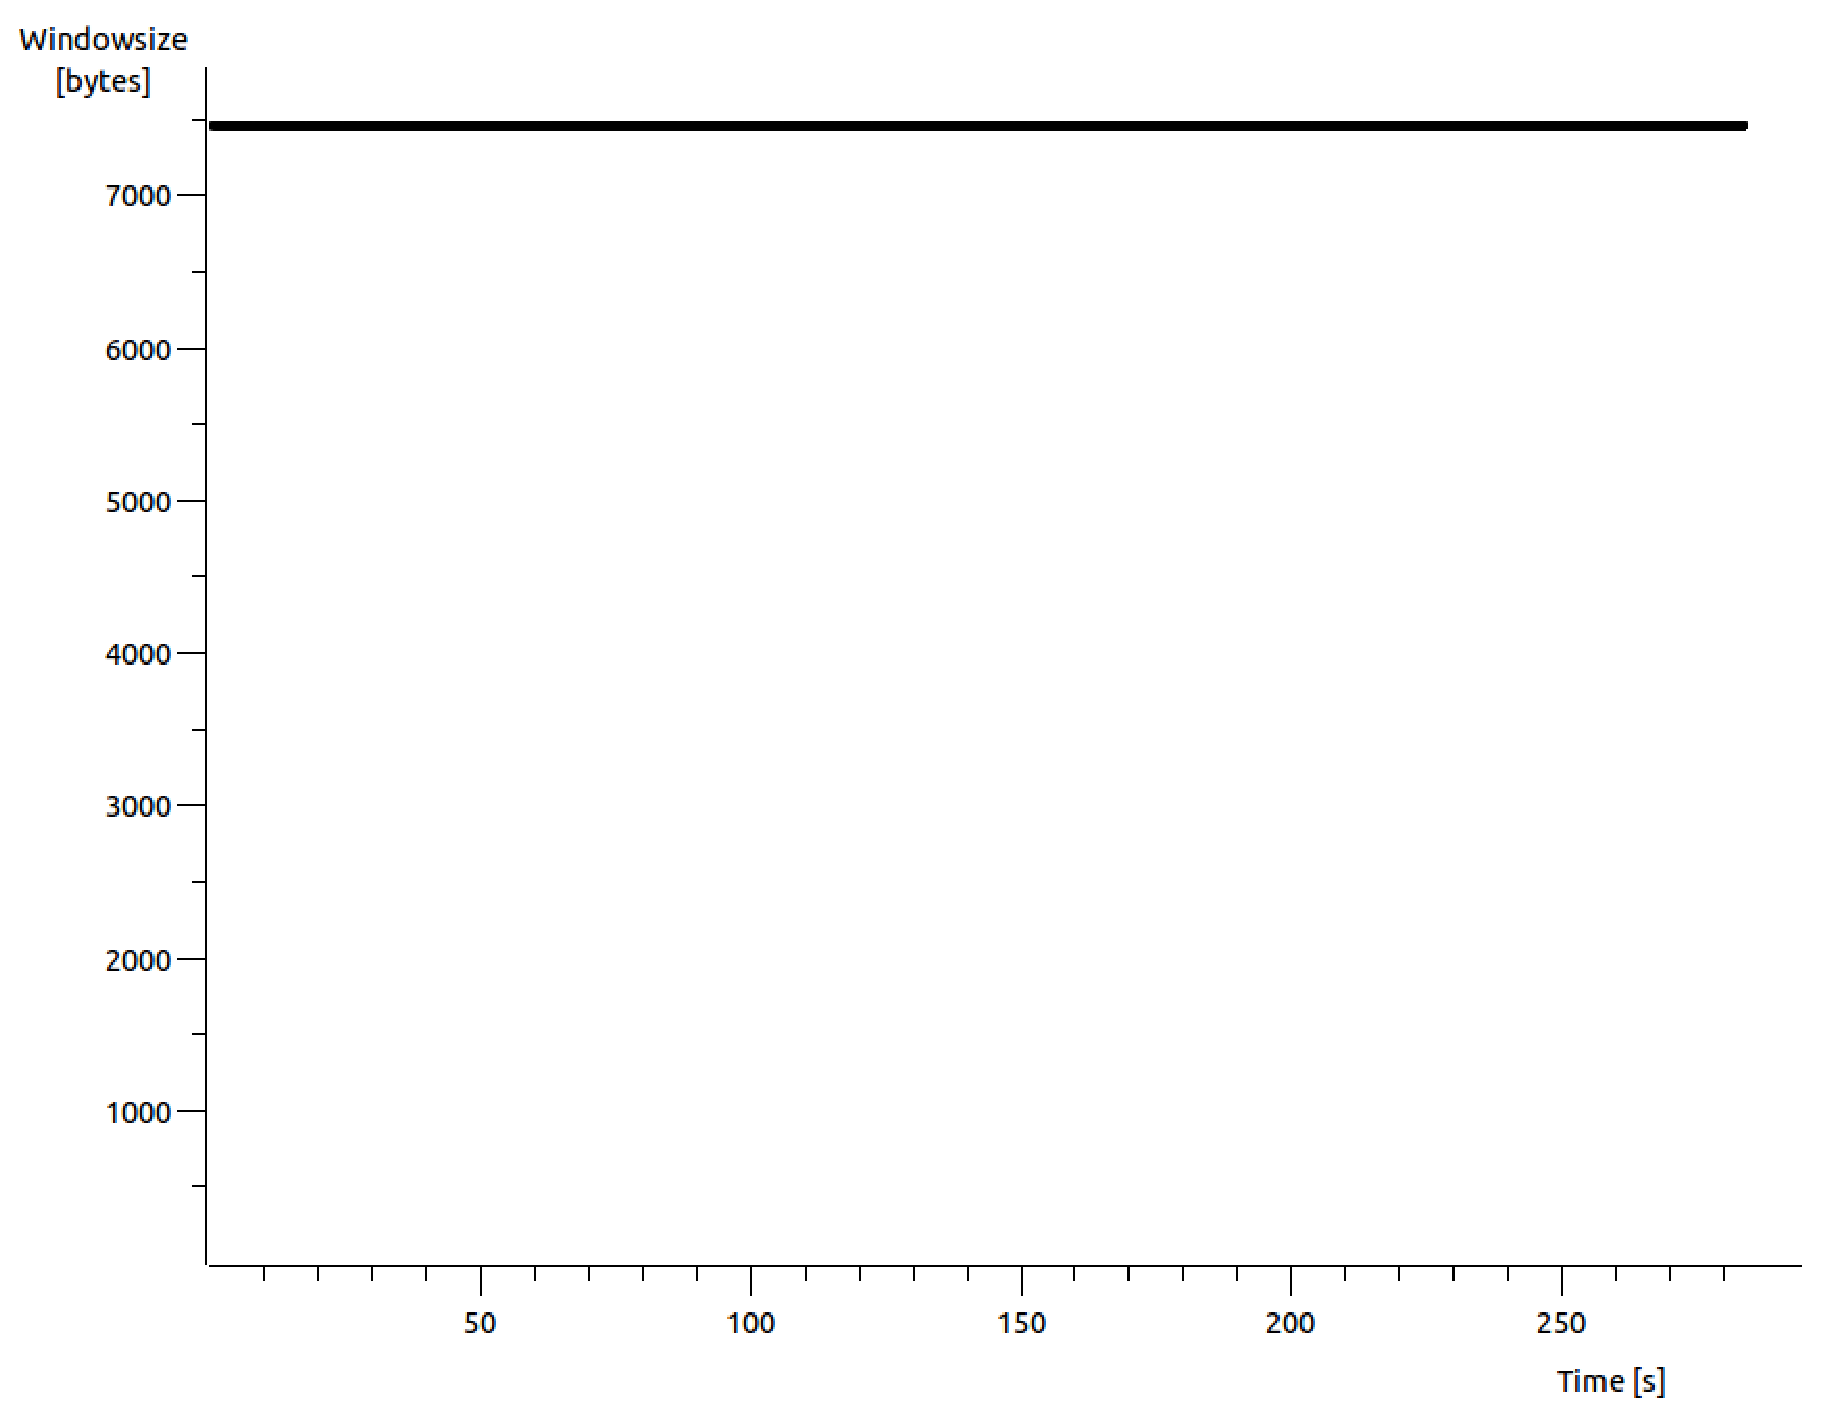
\includegraphics[width=\textwidth]{s4-1_wnd}
  \caption{Window size}
 \end{subfigure}
 \begin{subfigure}[b]{0.2\textwidth}
  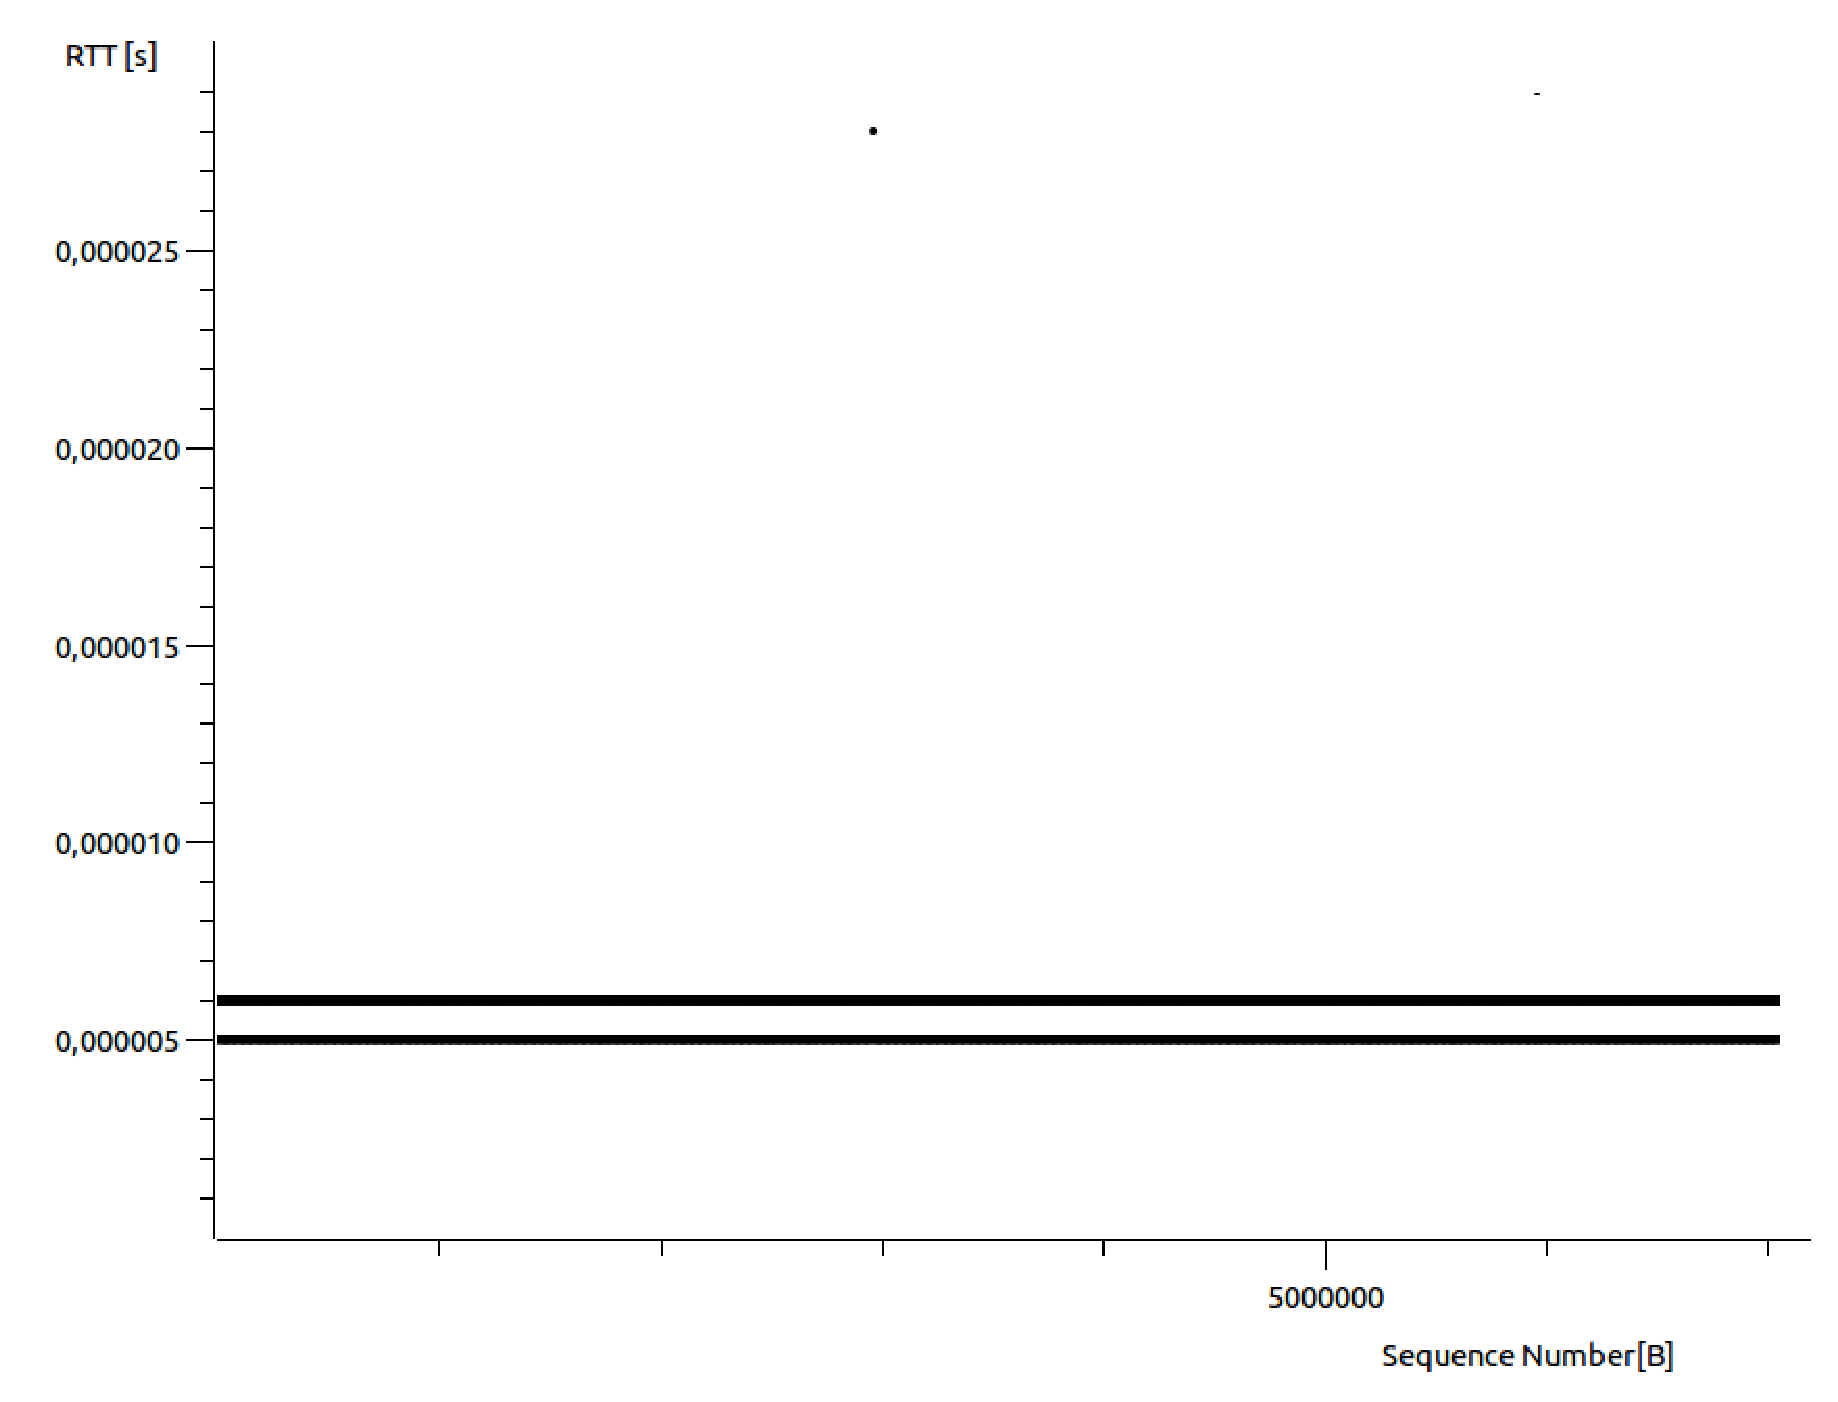
\includegraphics[width=\textwidth]{s4-1_rtt}
  \caption{RTT}
 \end{subfigure}
 \caption{Scene 4-1: TCP New Reno + 50 ms delay}
\end{figure}

\begin{figure}
 \centering
 \begin{subfigure}[b]{0.2\textwidth}
  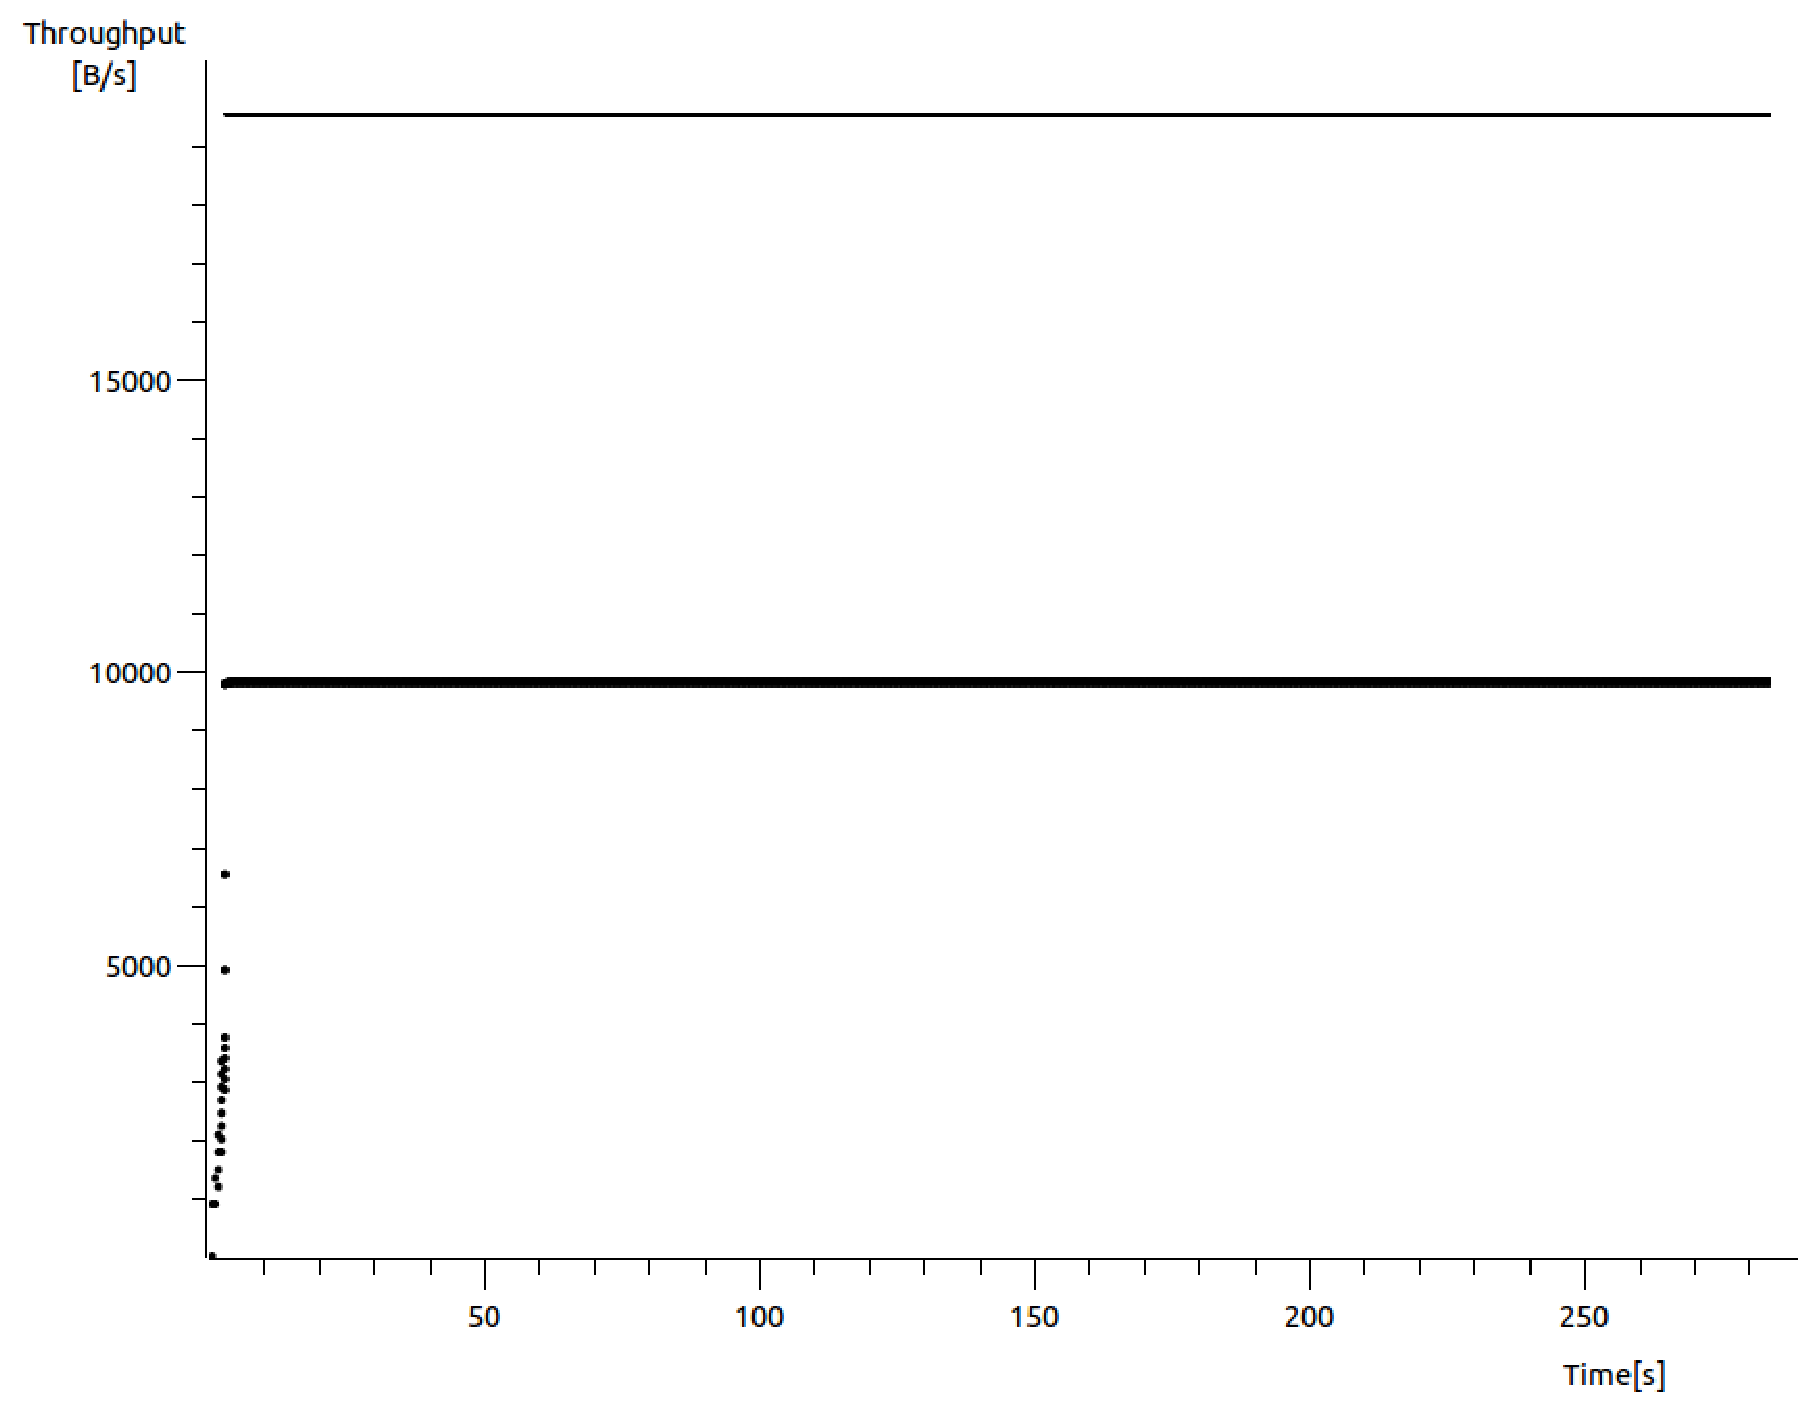
\includegraphics[width=\textwidth]{s4-2_thru}
  \caption{Throughput}
 \end{subfigure}
 \begin{subfigure}[b]{0.2\textwidth}
  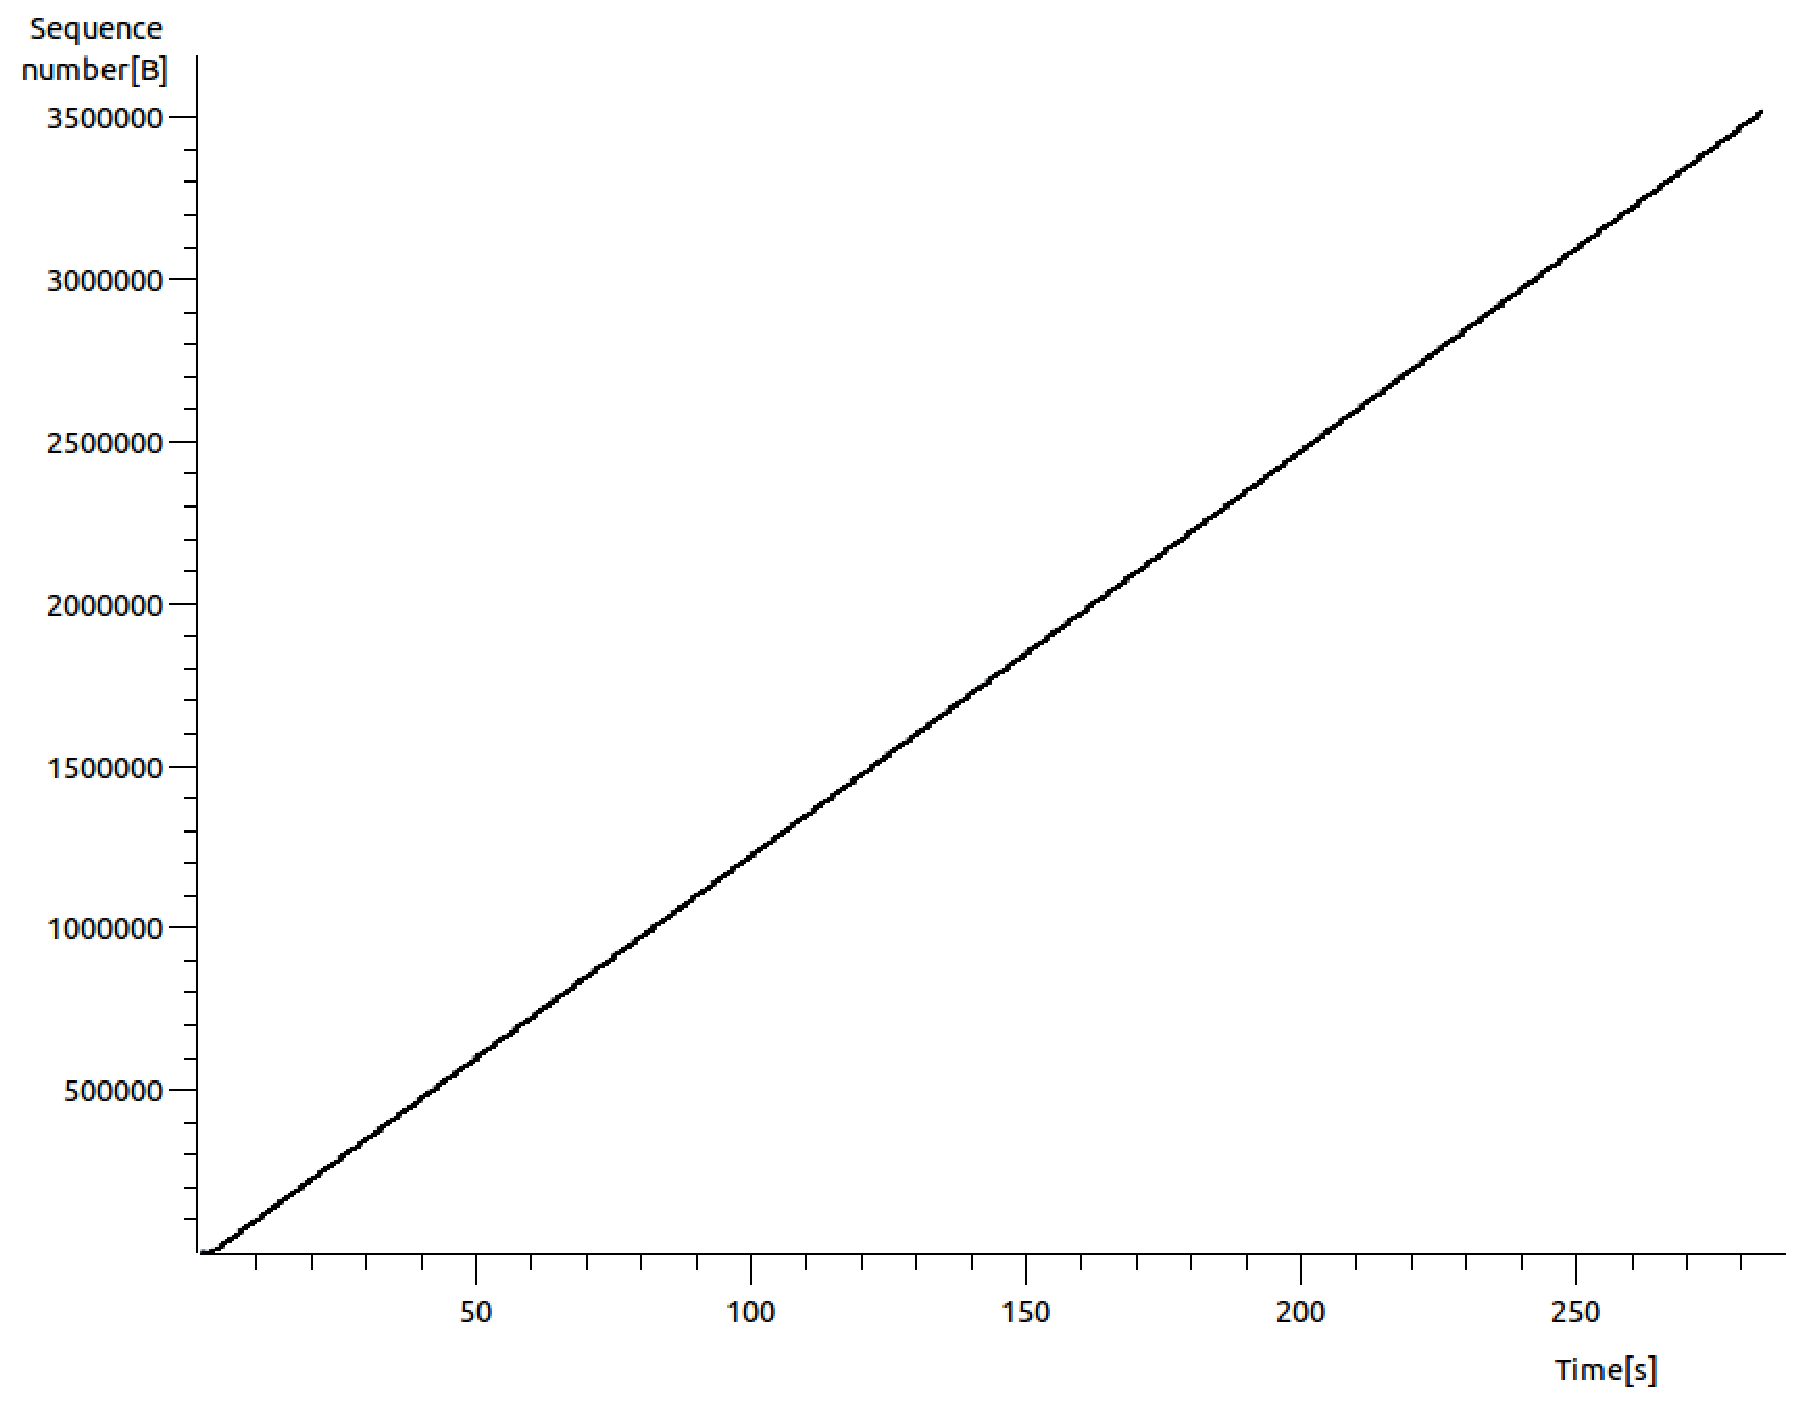
\includegraphics[width=\textwidth]{s4-2_seq}
  \caption{TCP sequence}
 \end{subfigure}
 \begin{subfigure}[b]{0.2\textwidth}
  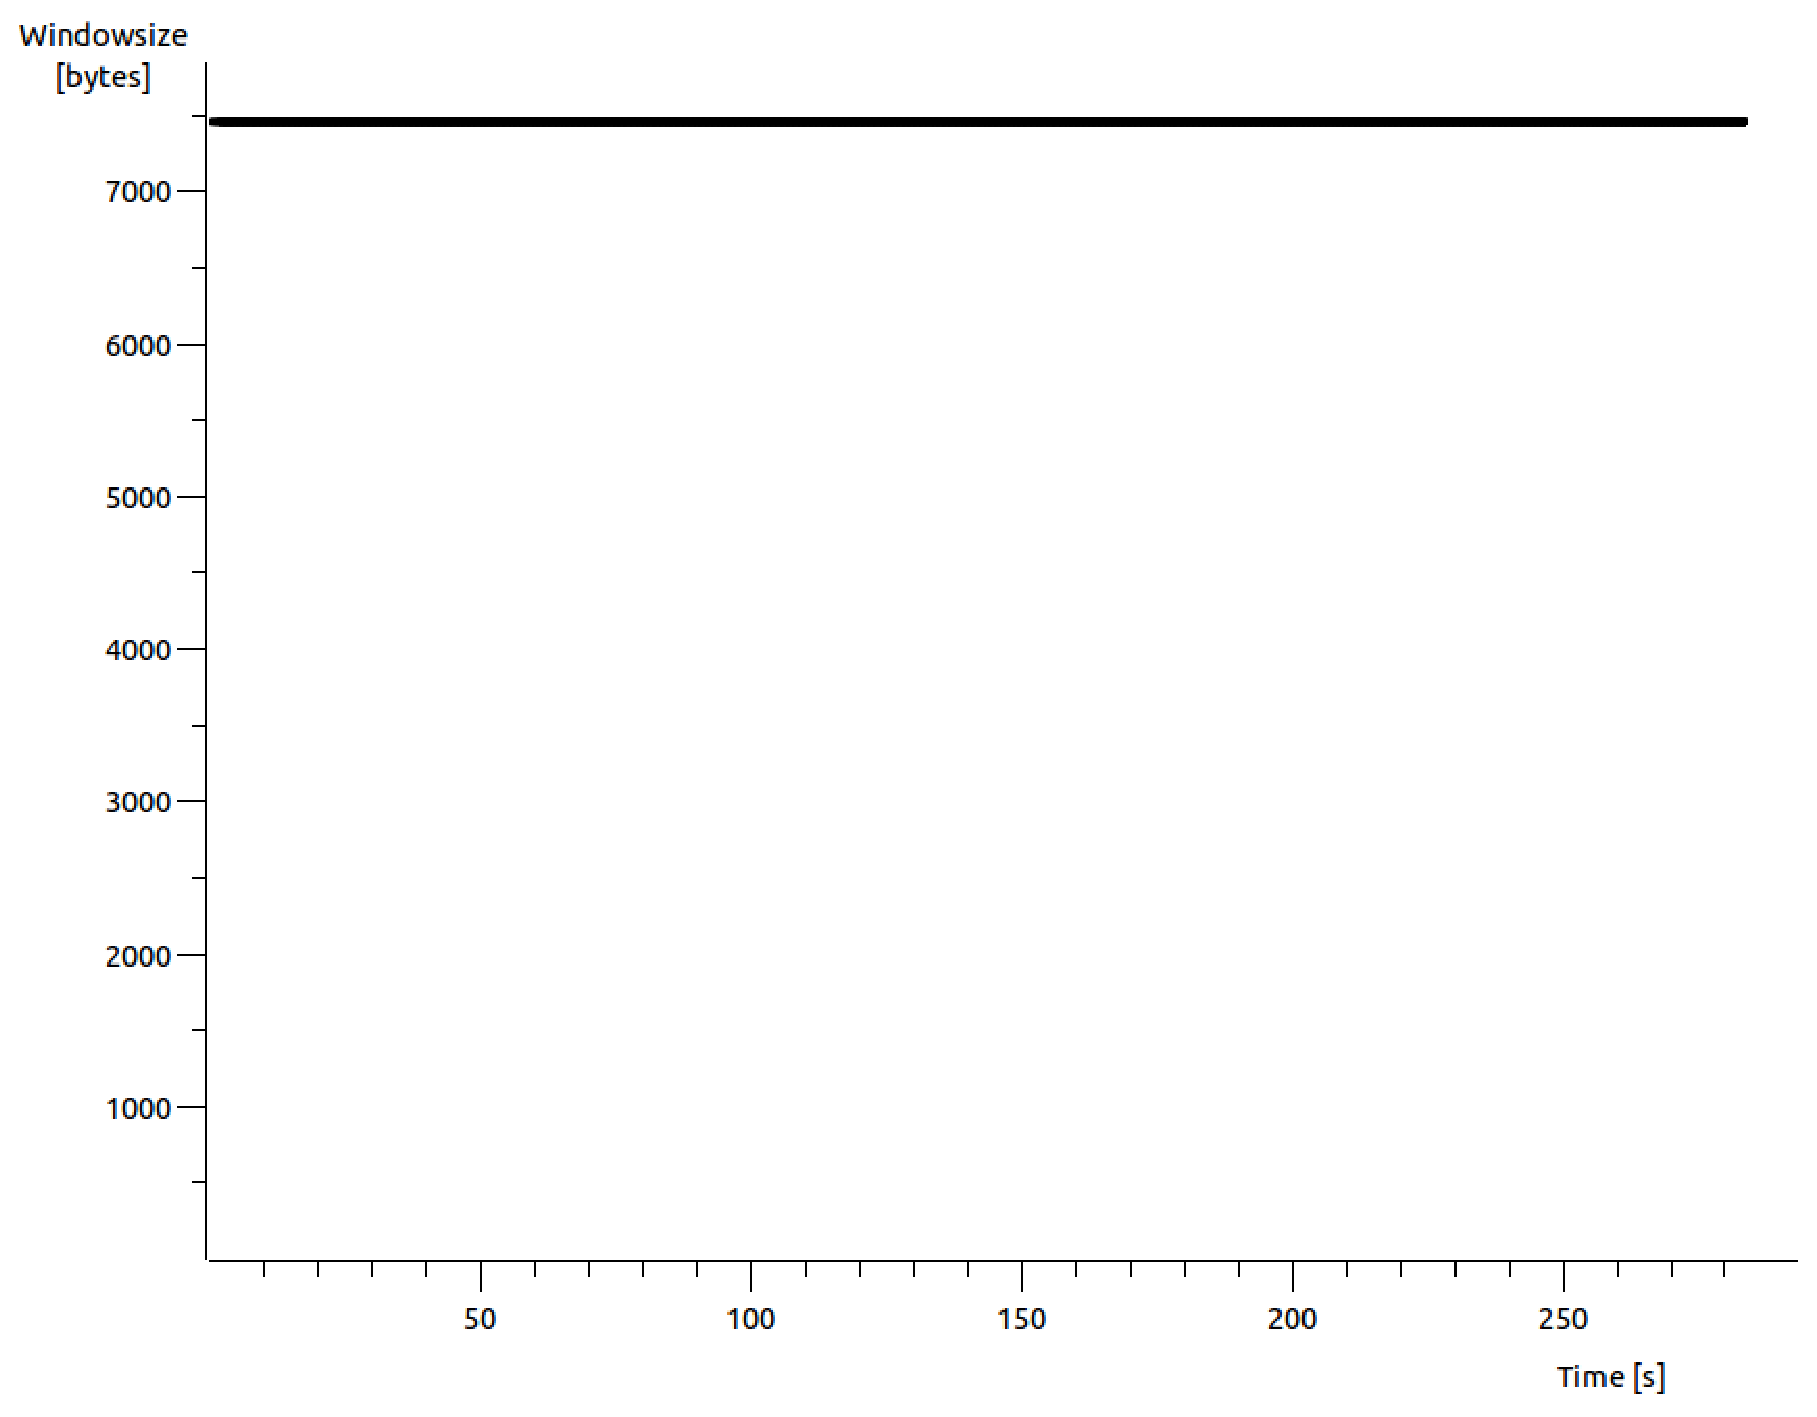
\includegraphics[width=\textwidth]{s4-2_wnd}
  \caption{Window size}
 \end{subfigure}
 \begin{subfigure}[b]{0.2\textwidth}
  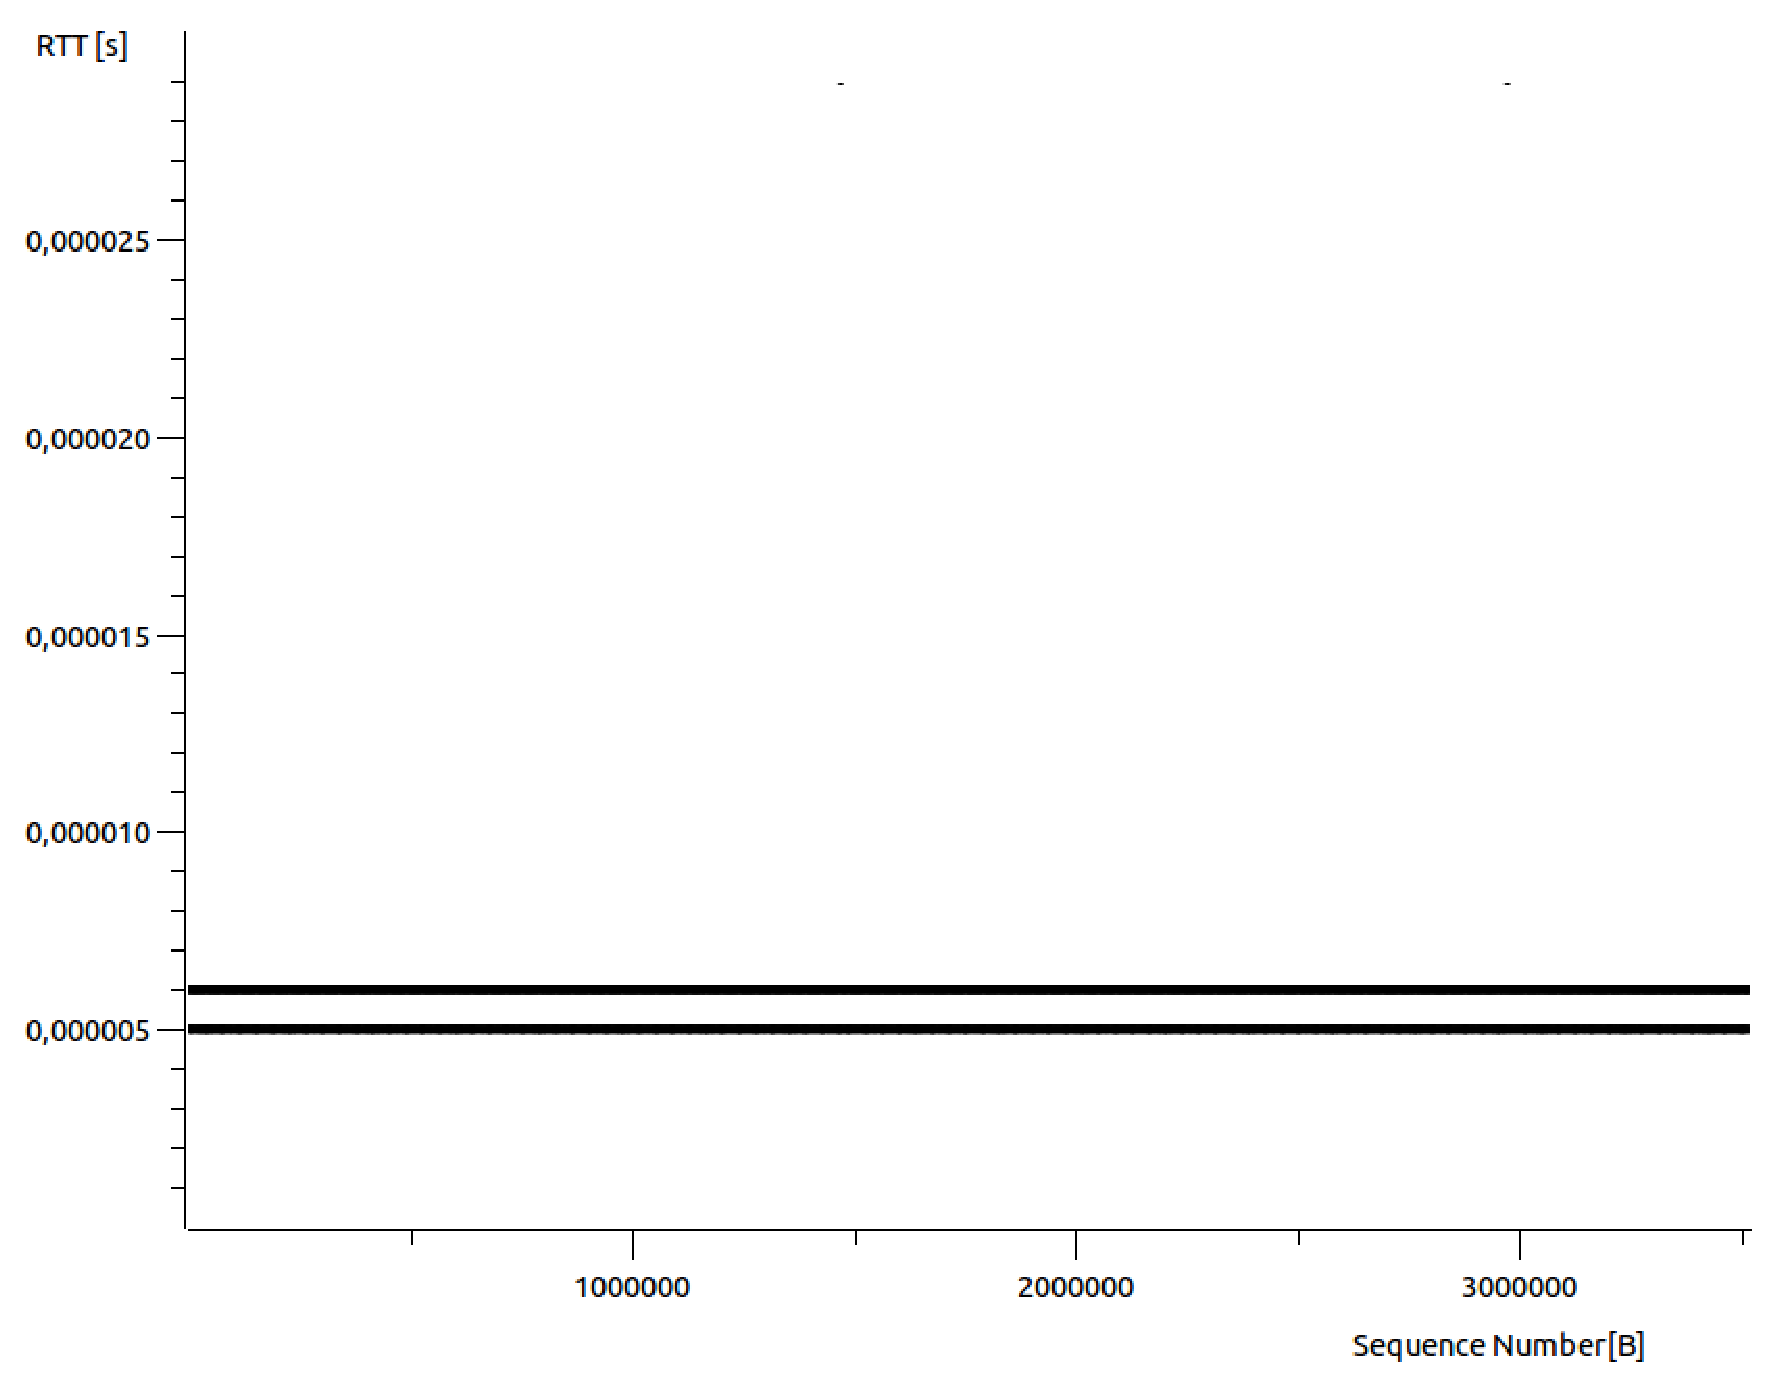
\includegraphics[width=\textwidth]{s4-2_rtt}
  \caption{RTT}
 \end{subfigure}
 \caption{Scene 4-2: TCP New Reno + 200 ms delay}
\end{figure}

\begin{figure}
 \centering
 \begin{subfigure}[b]{0.2\textwidth}
  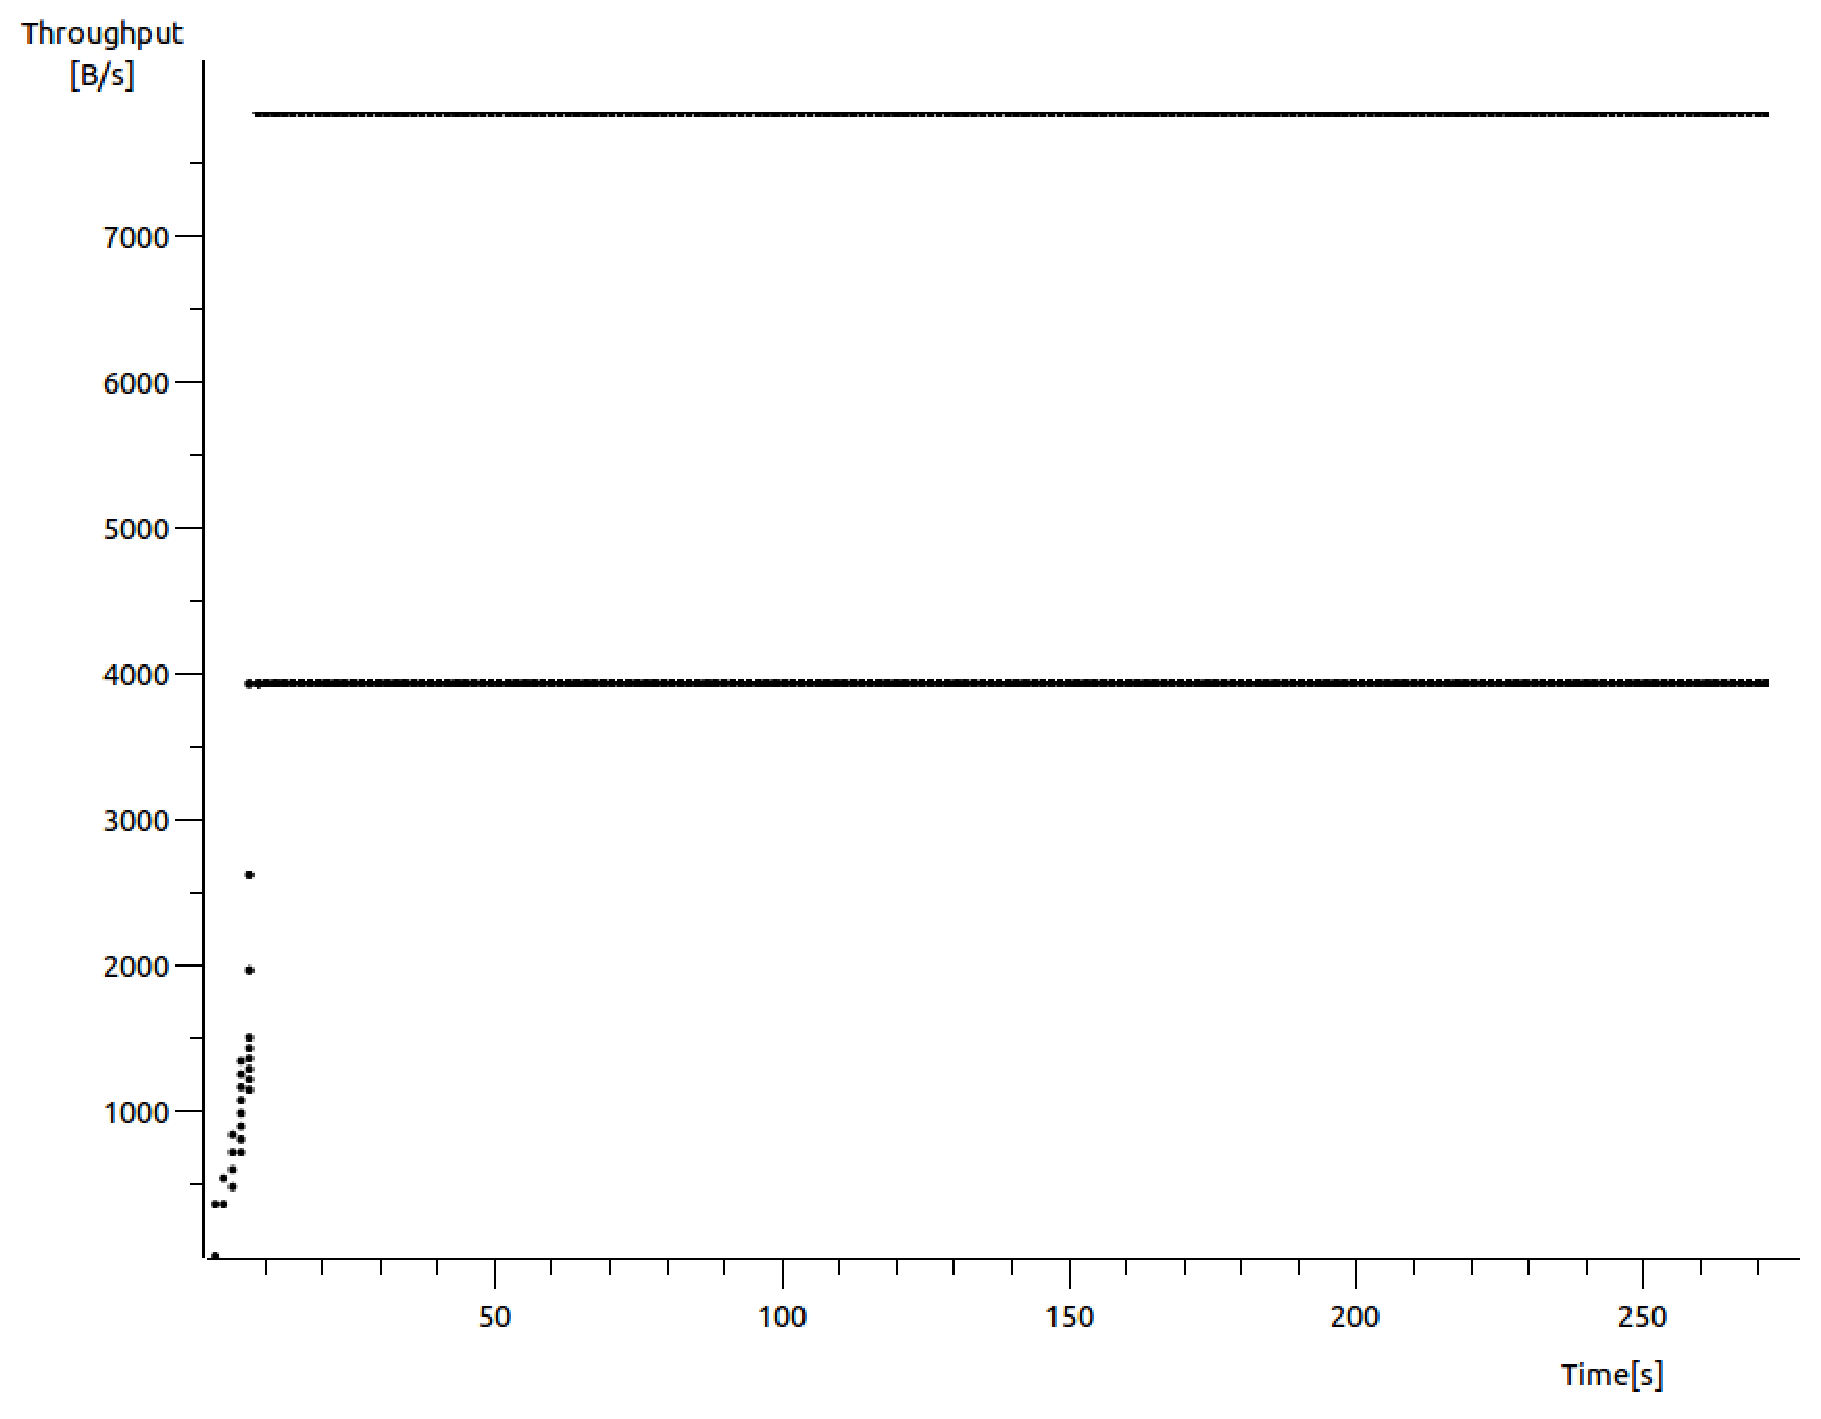
\includegraphics[width=\textwidth]{s4-3_thru}
  \caption{Throughput}
 \end{subfigure}
 \begin{subfigure}[b]{0.2\textwidth}
  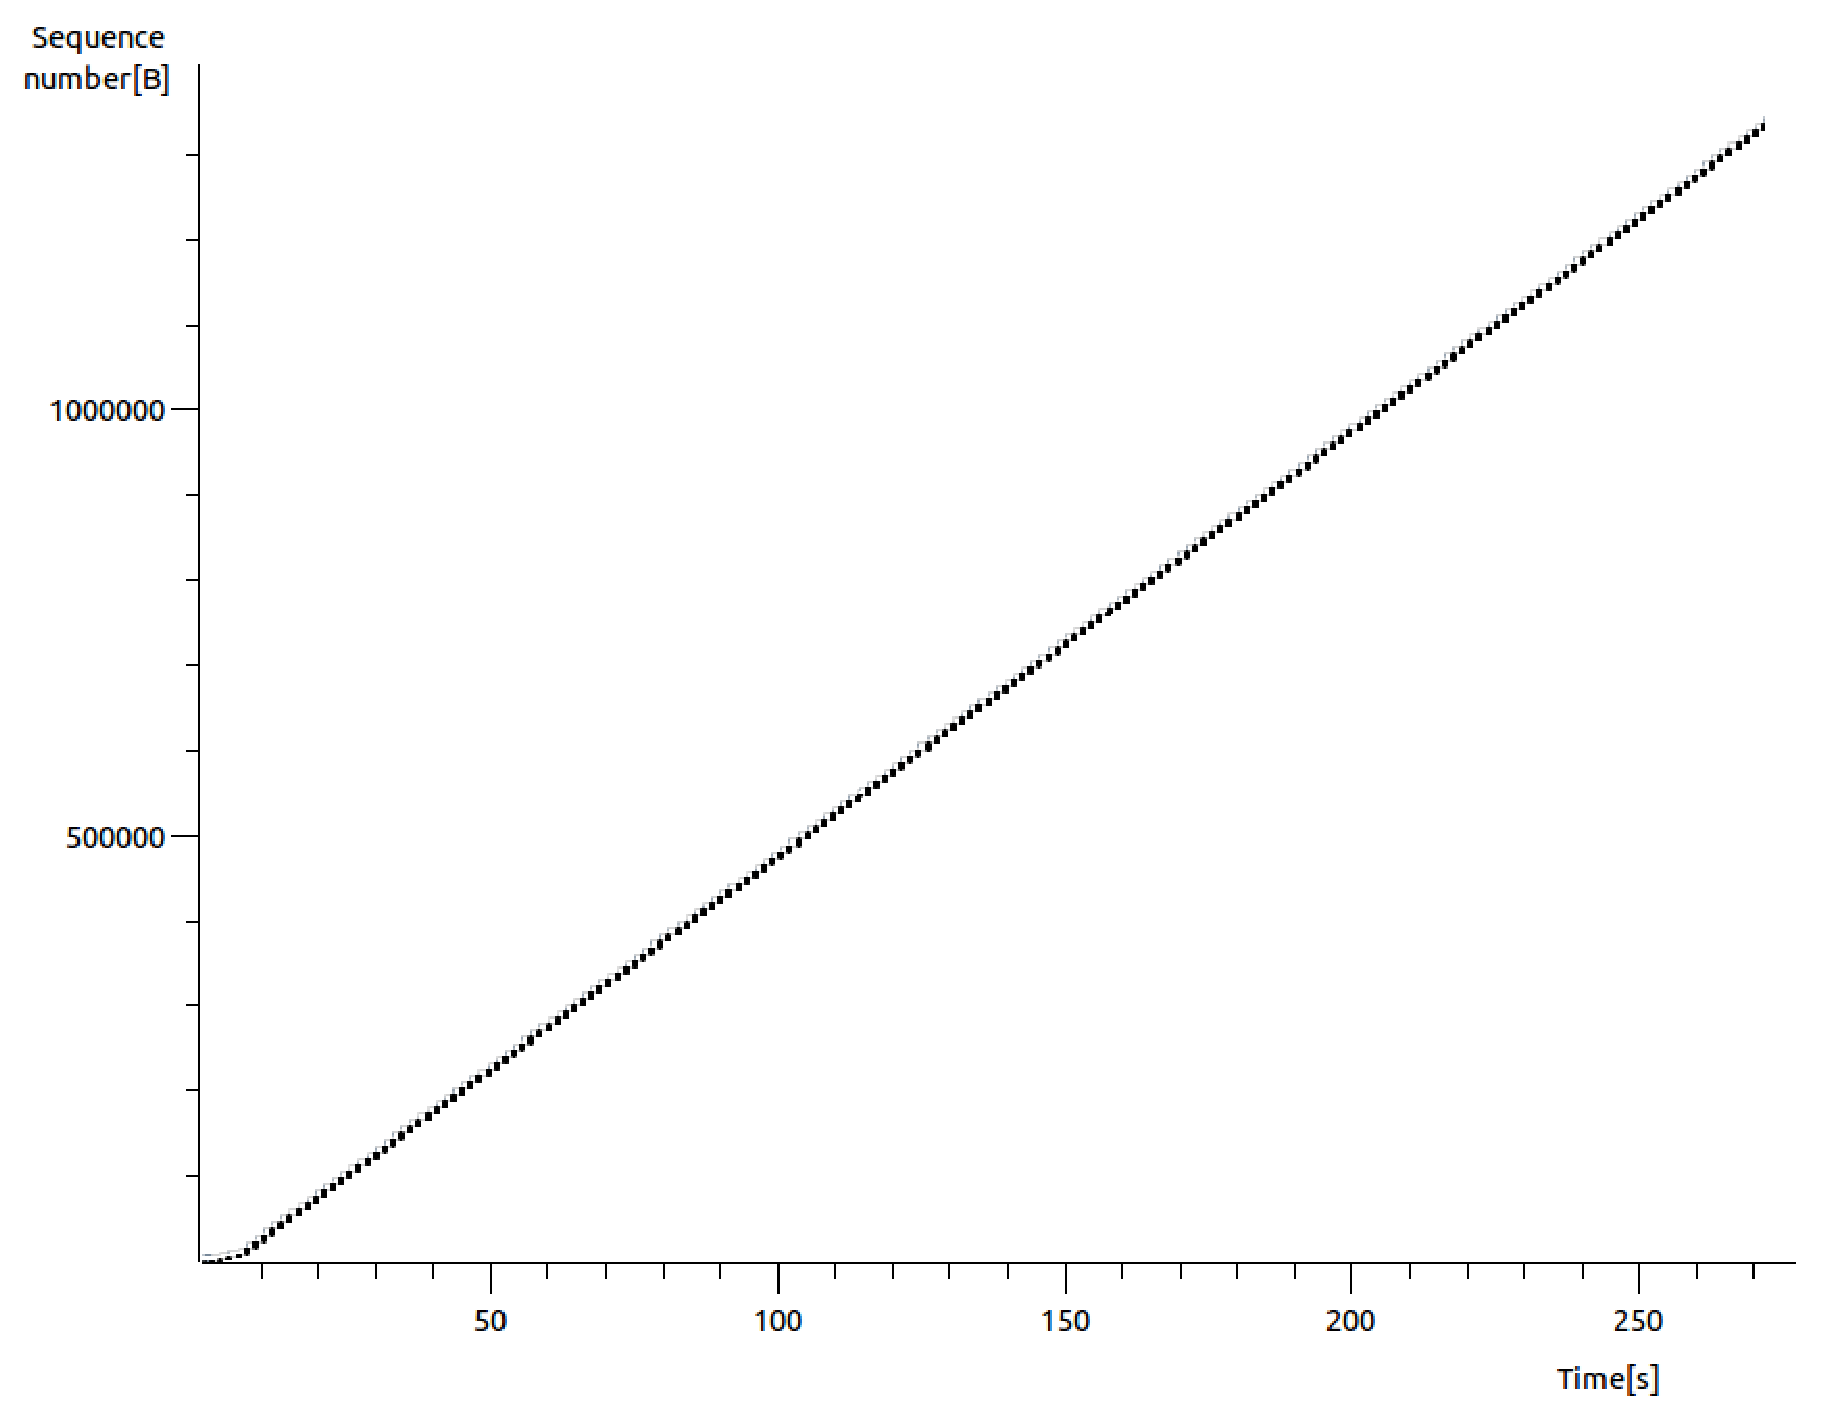
\includegraphics[width=\textwidth]{s4-3_seq}
  \caption{TCP sequence}
 \end{subfigure}
 \begin{subfigure}[b]{0.2\textwidth}
  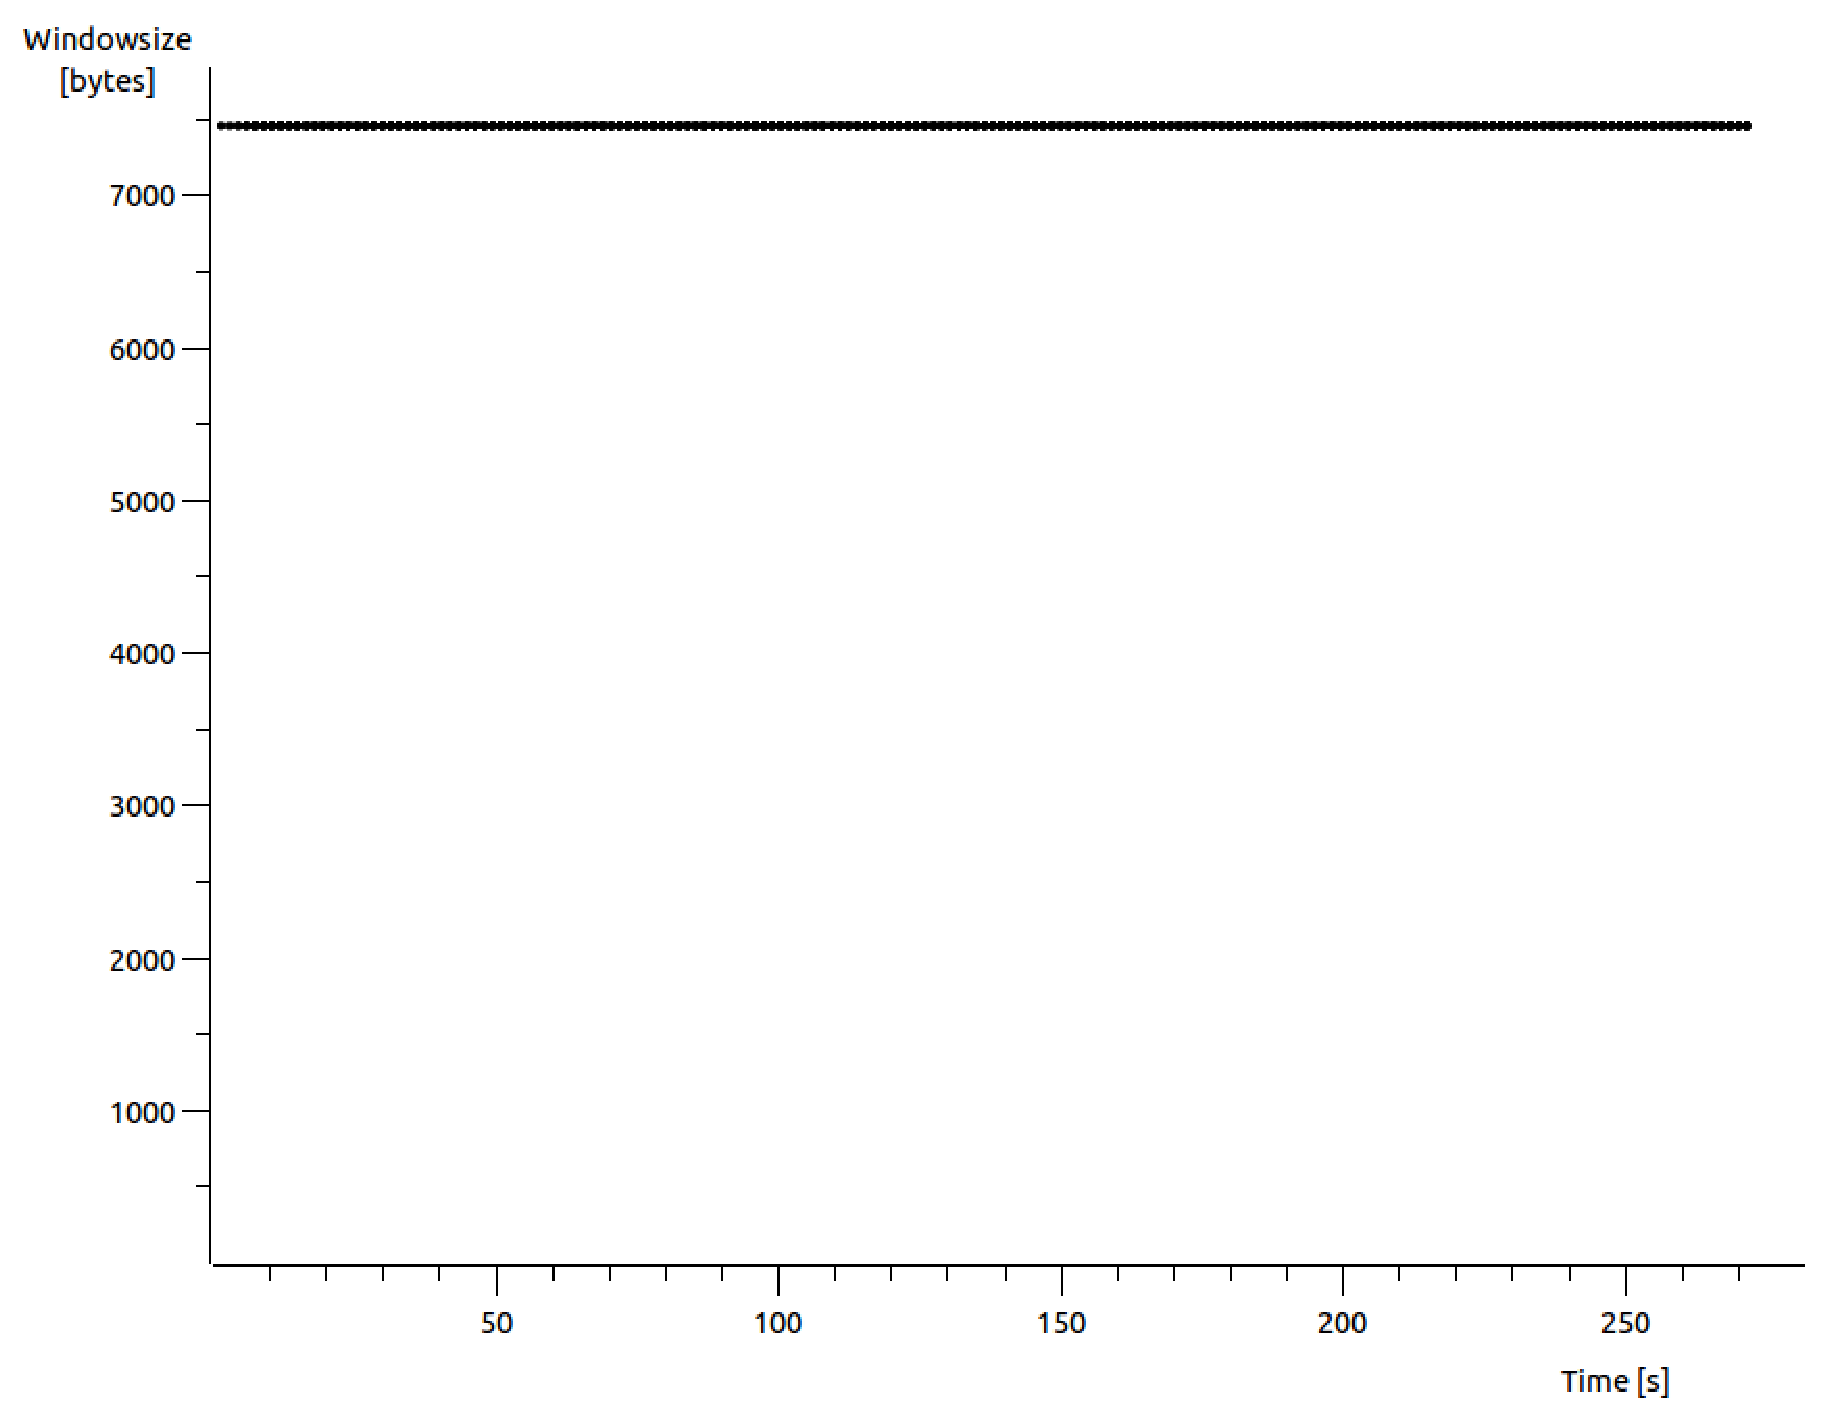
\includegraphics[width=\textwidth]{s4-3_wnd}
  \caption{Window size}
 \end{subfigure}
 \begin{subfigure}[b]{0.2\textwidth}
  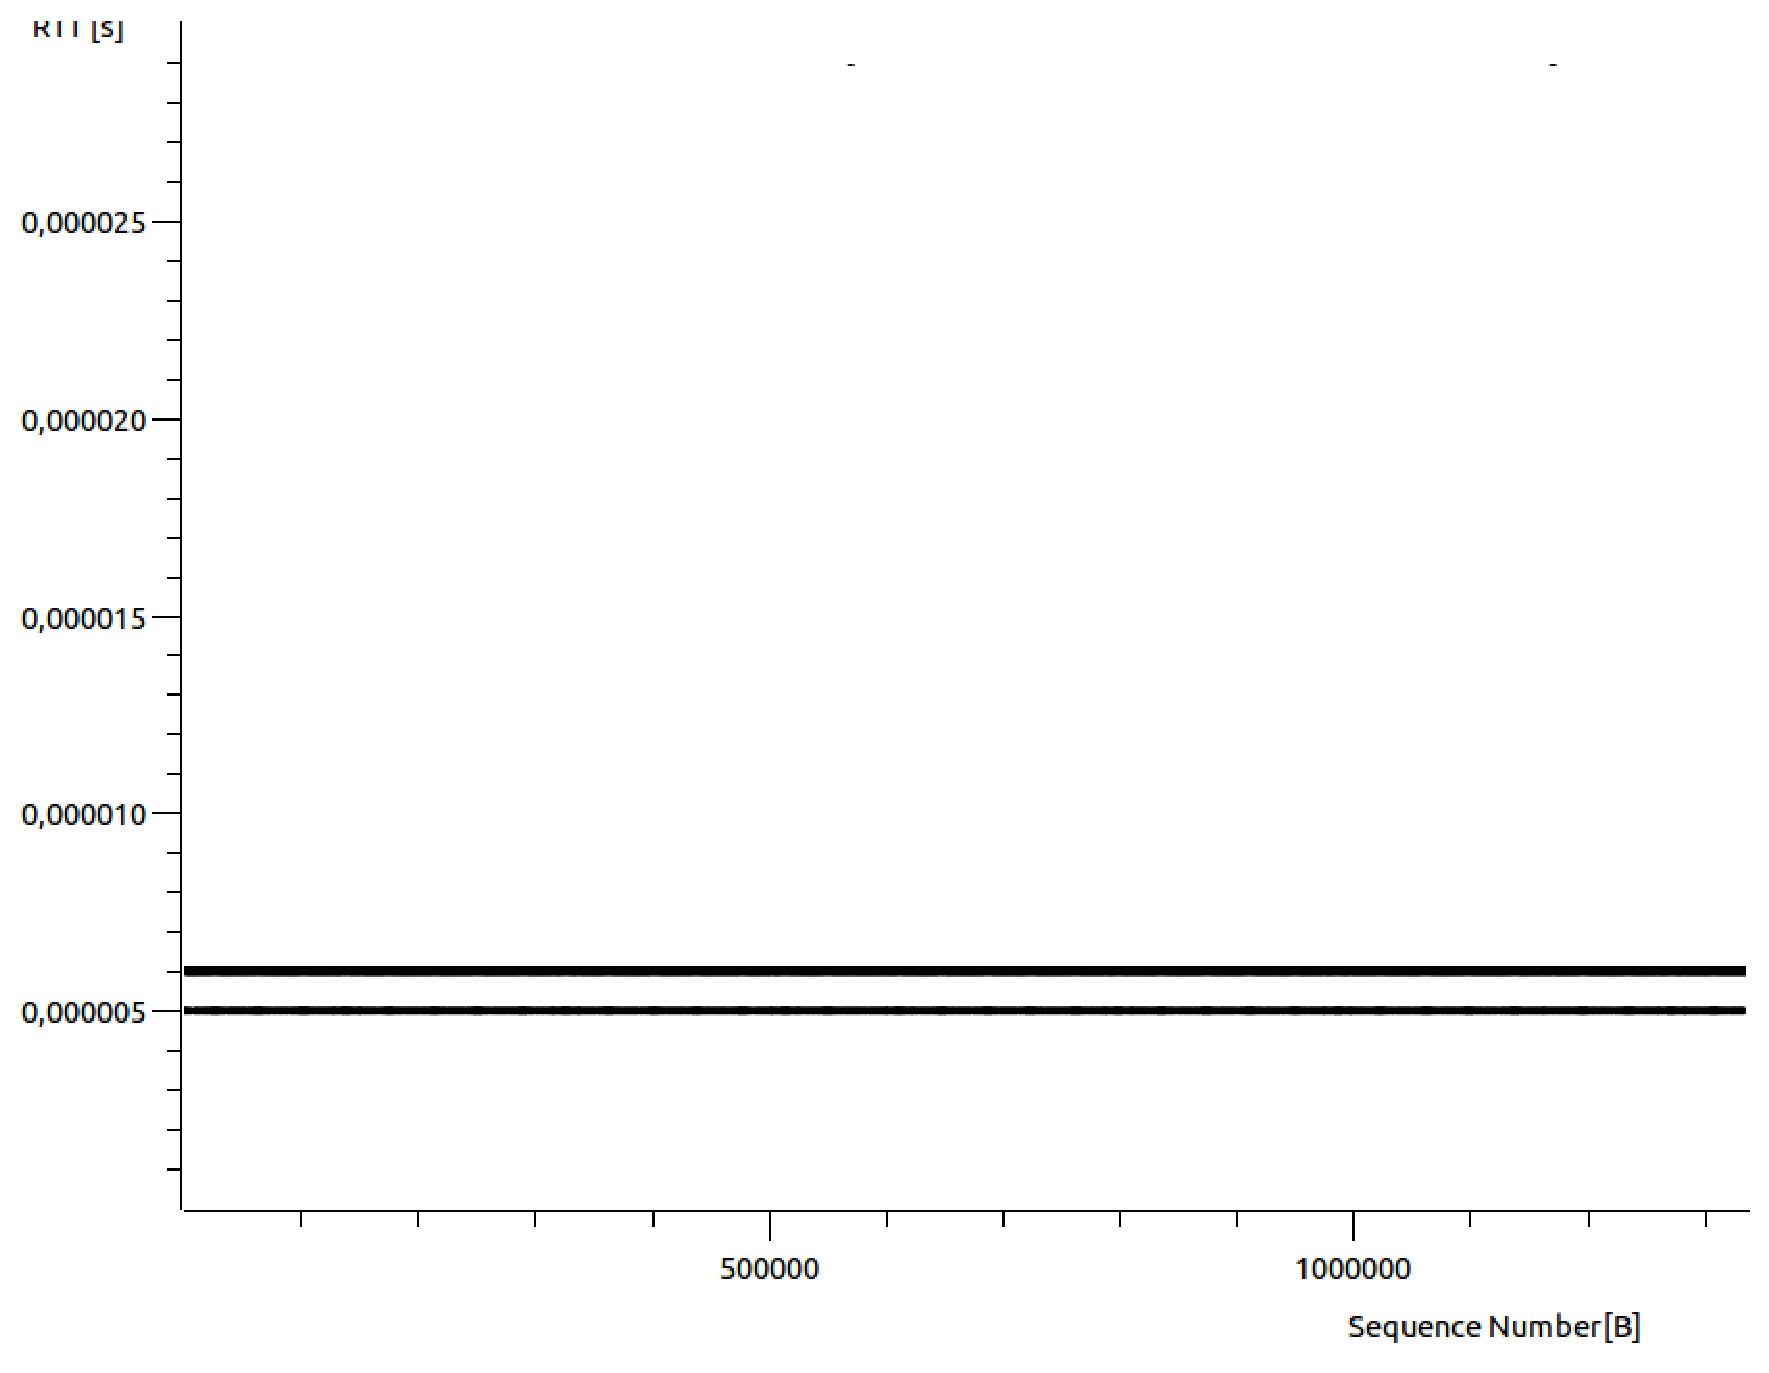
\includegraphics[width=\textwidth]{s4-3_rtt}
  \caption{RTT}
 \end{subfigure}
 \caption{Scene 4-3: TCP New Reno + 250 delay}
\end{figure}

\begin{figure}
 \centering
 \begin{subfigure}[b]{0.2\textwidth}
  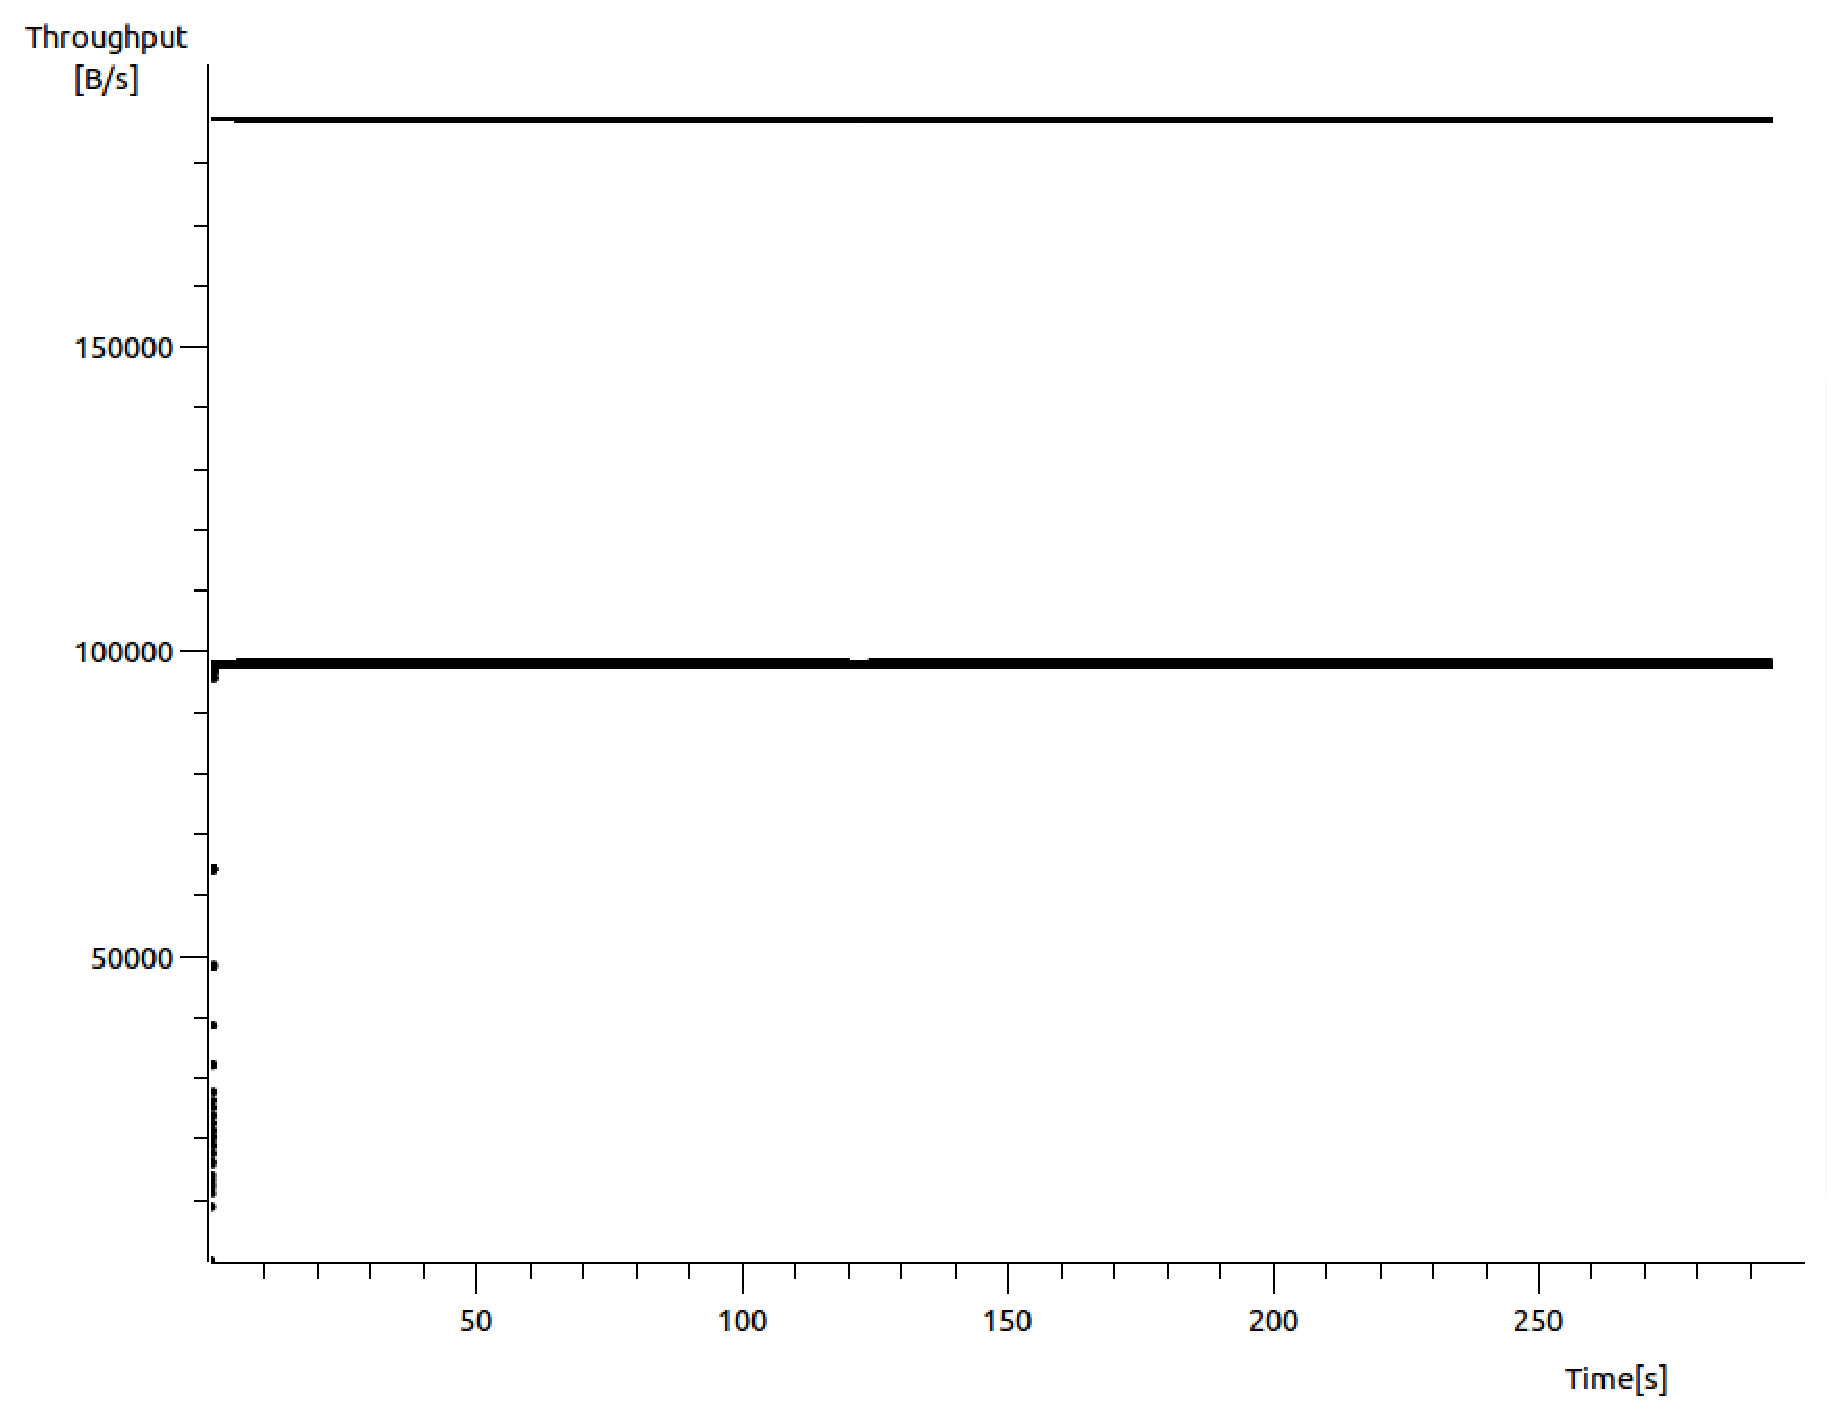
\includegraphics[width=\textwidth]{s7-0_th}
  \caption{Throughput}
 \end{subfigure}
 \begin{subfigure}[b]{0.2\textwidth}
  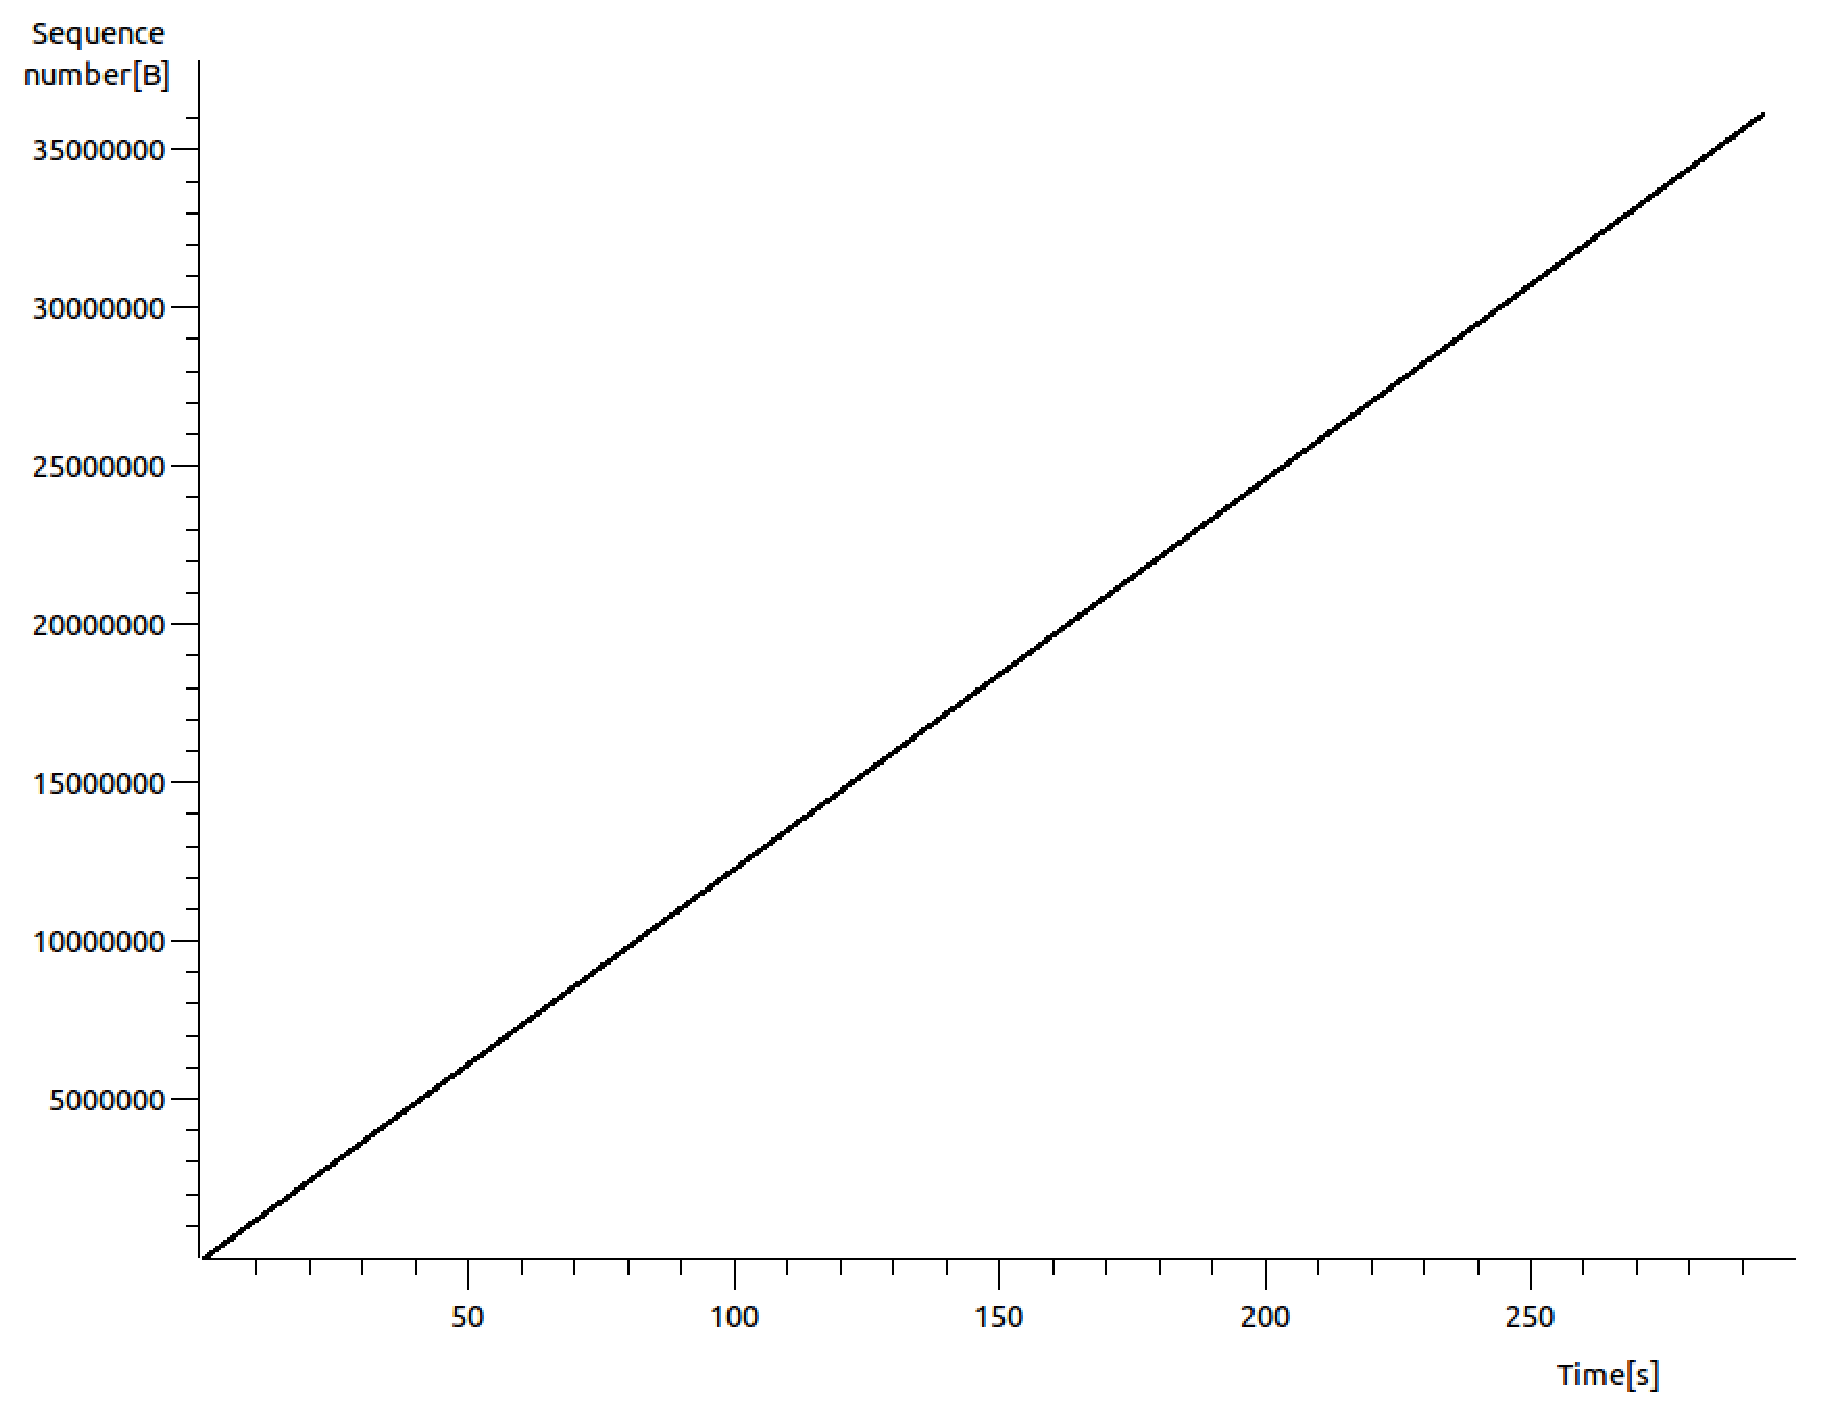
\includegraphics[width=\textwidth]{s7-0_seq}
  \caption{TCP sequence}
 \end{subfigure}
 \begin{subfigure}[b]{0.2\textwidth}
  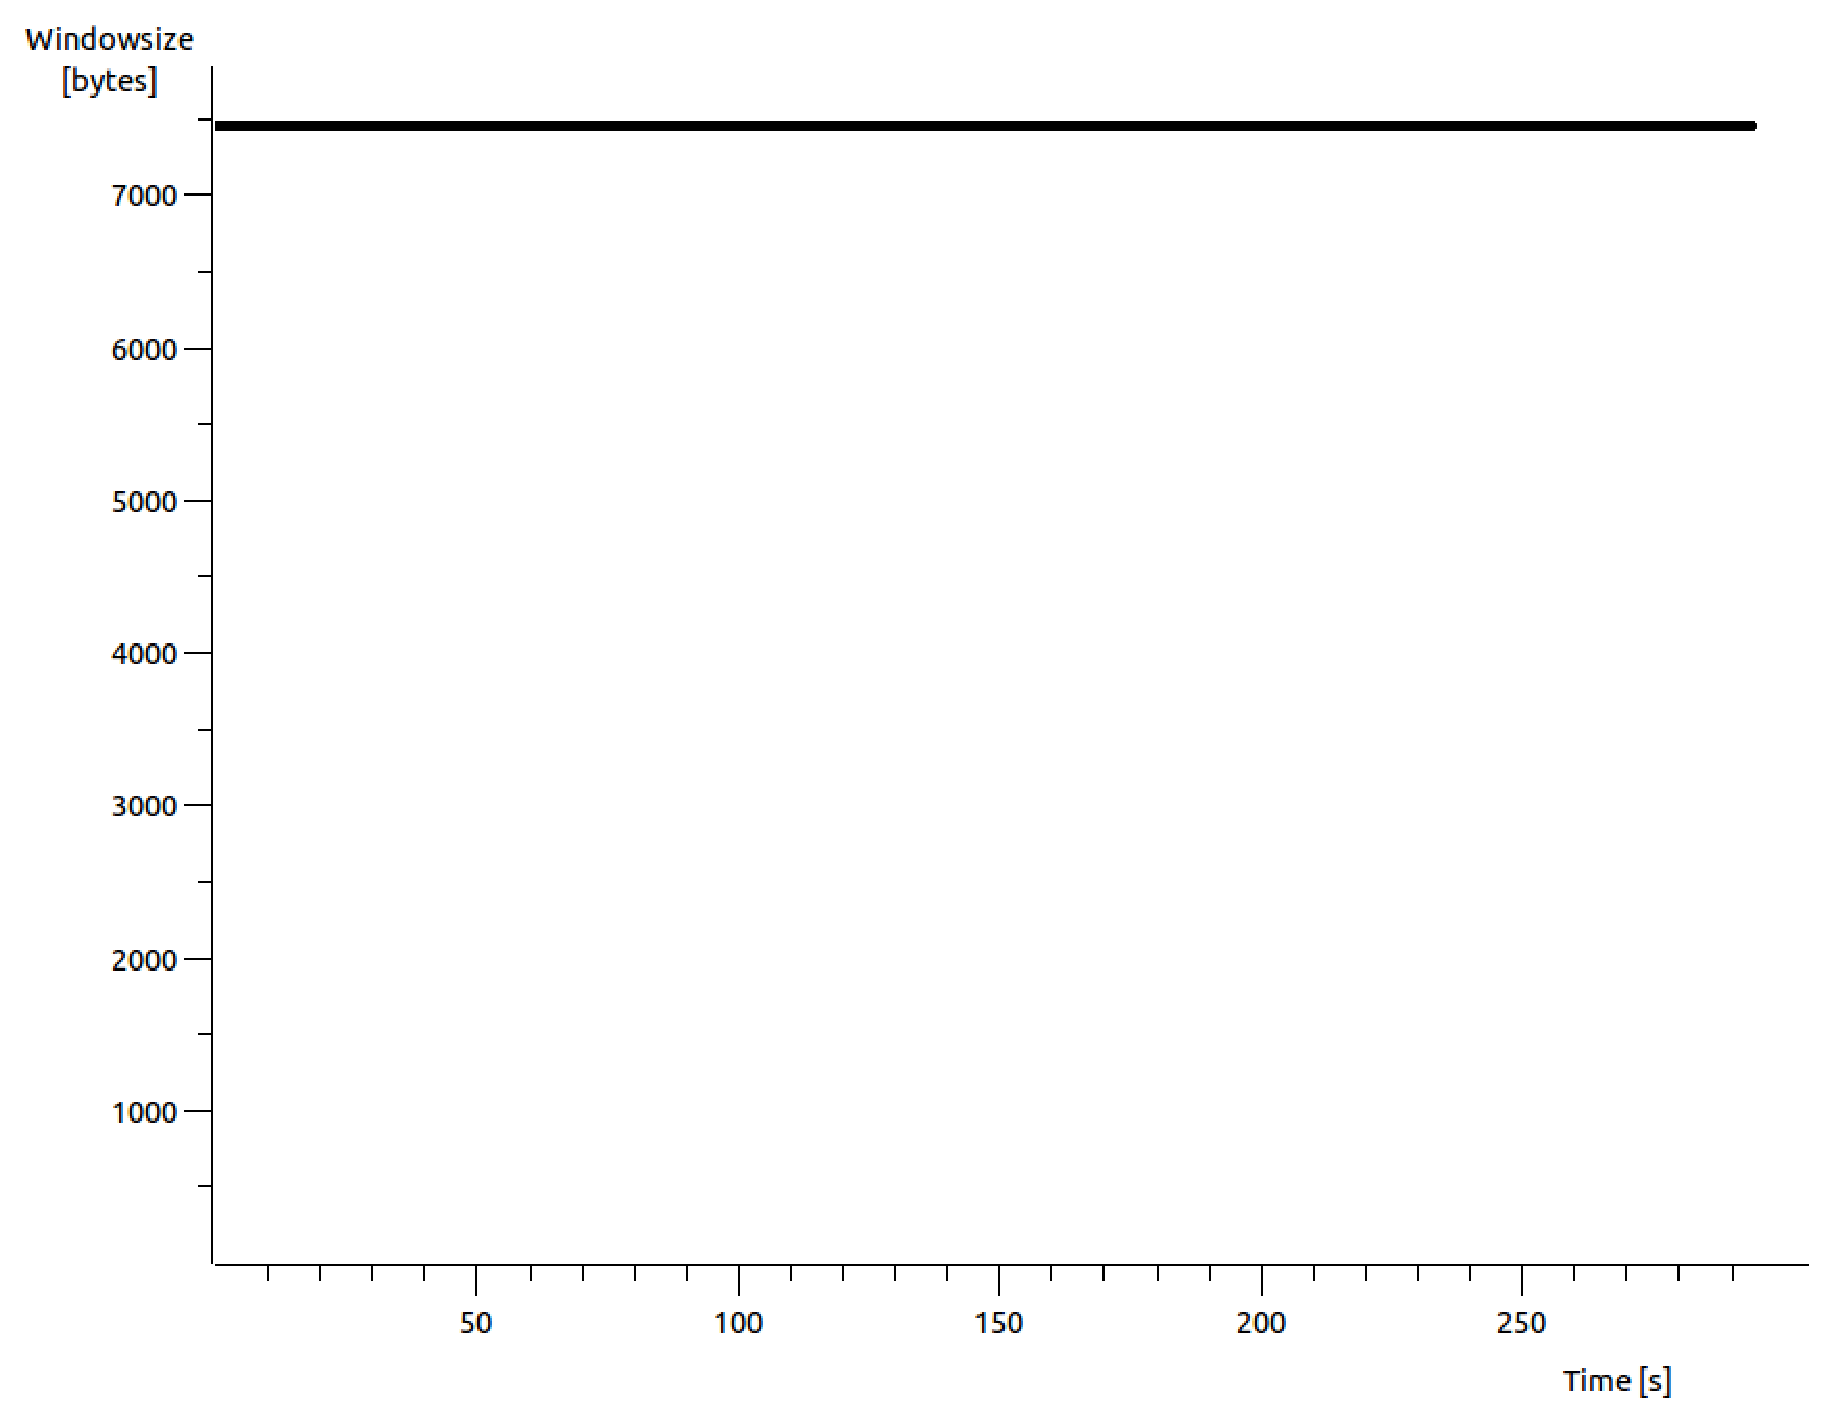
\includegraphics[width=\textwidth]{s7-0_wsize}
  \caption{Window size}
 \end{subfigure}
 \begin{subfigure}[b]{0.2\textwidth}
  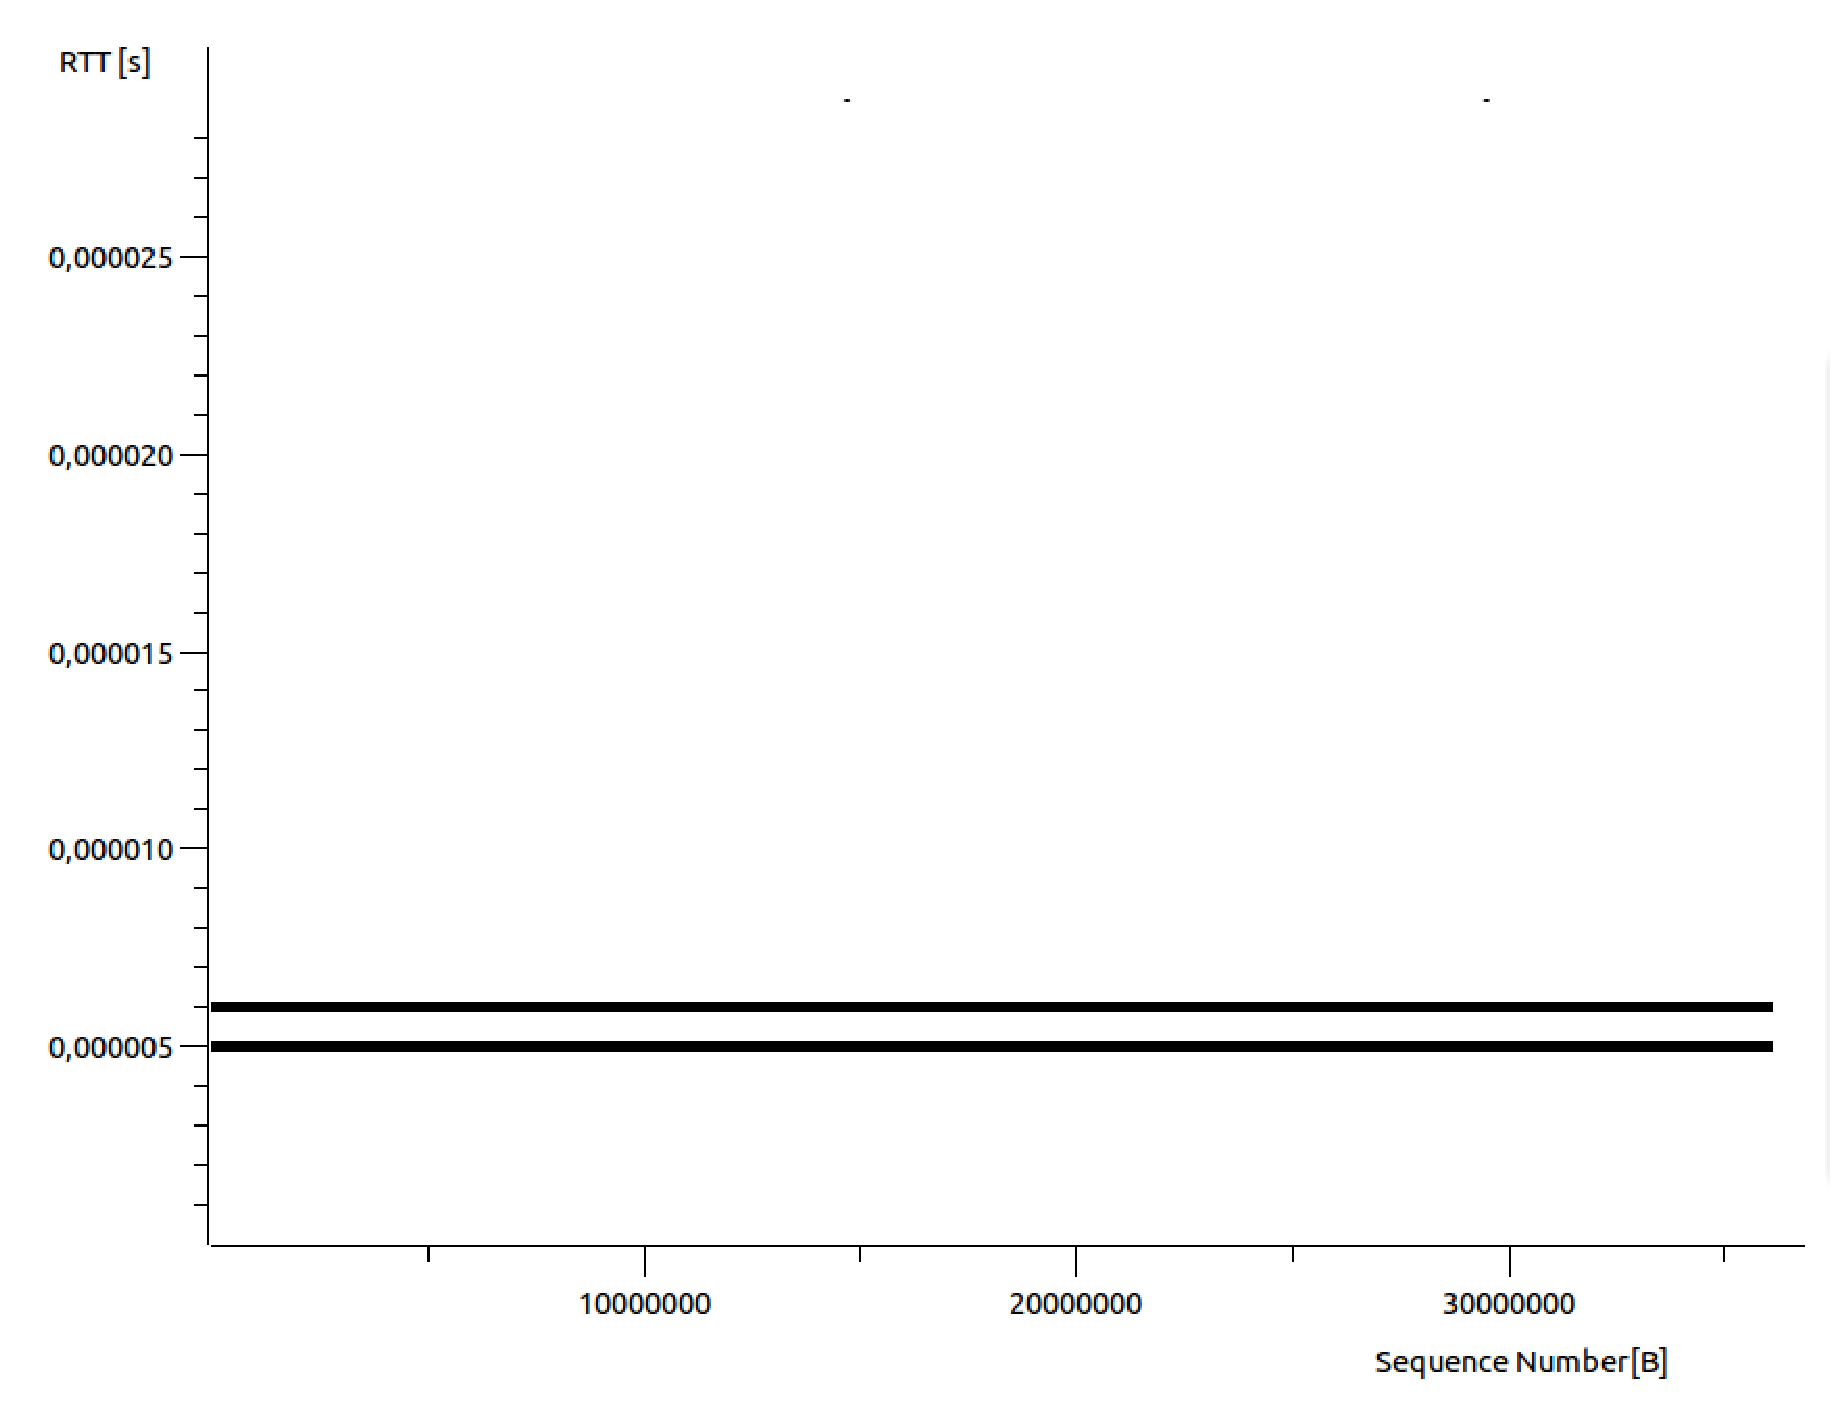
\includegraphics[width=\textwidth]{s7-0_rtt}
  \caption{RTT}
 \end{subfigure}
 \caption{Scene 7-0: TCP Vegas + 10 ms delay}
\end{figure}

\begin{figure}
 \centering
 \begin{subfigure}[b]{0.2\textwidth}
  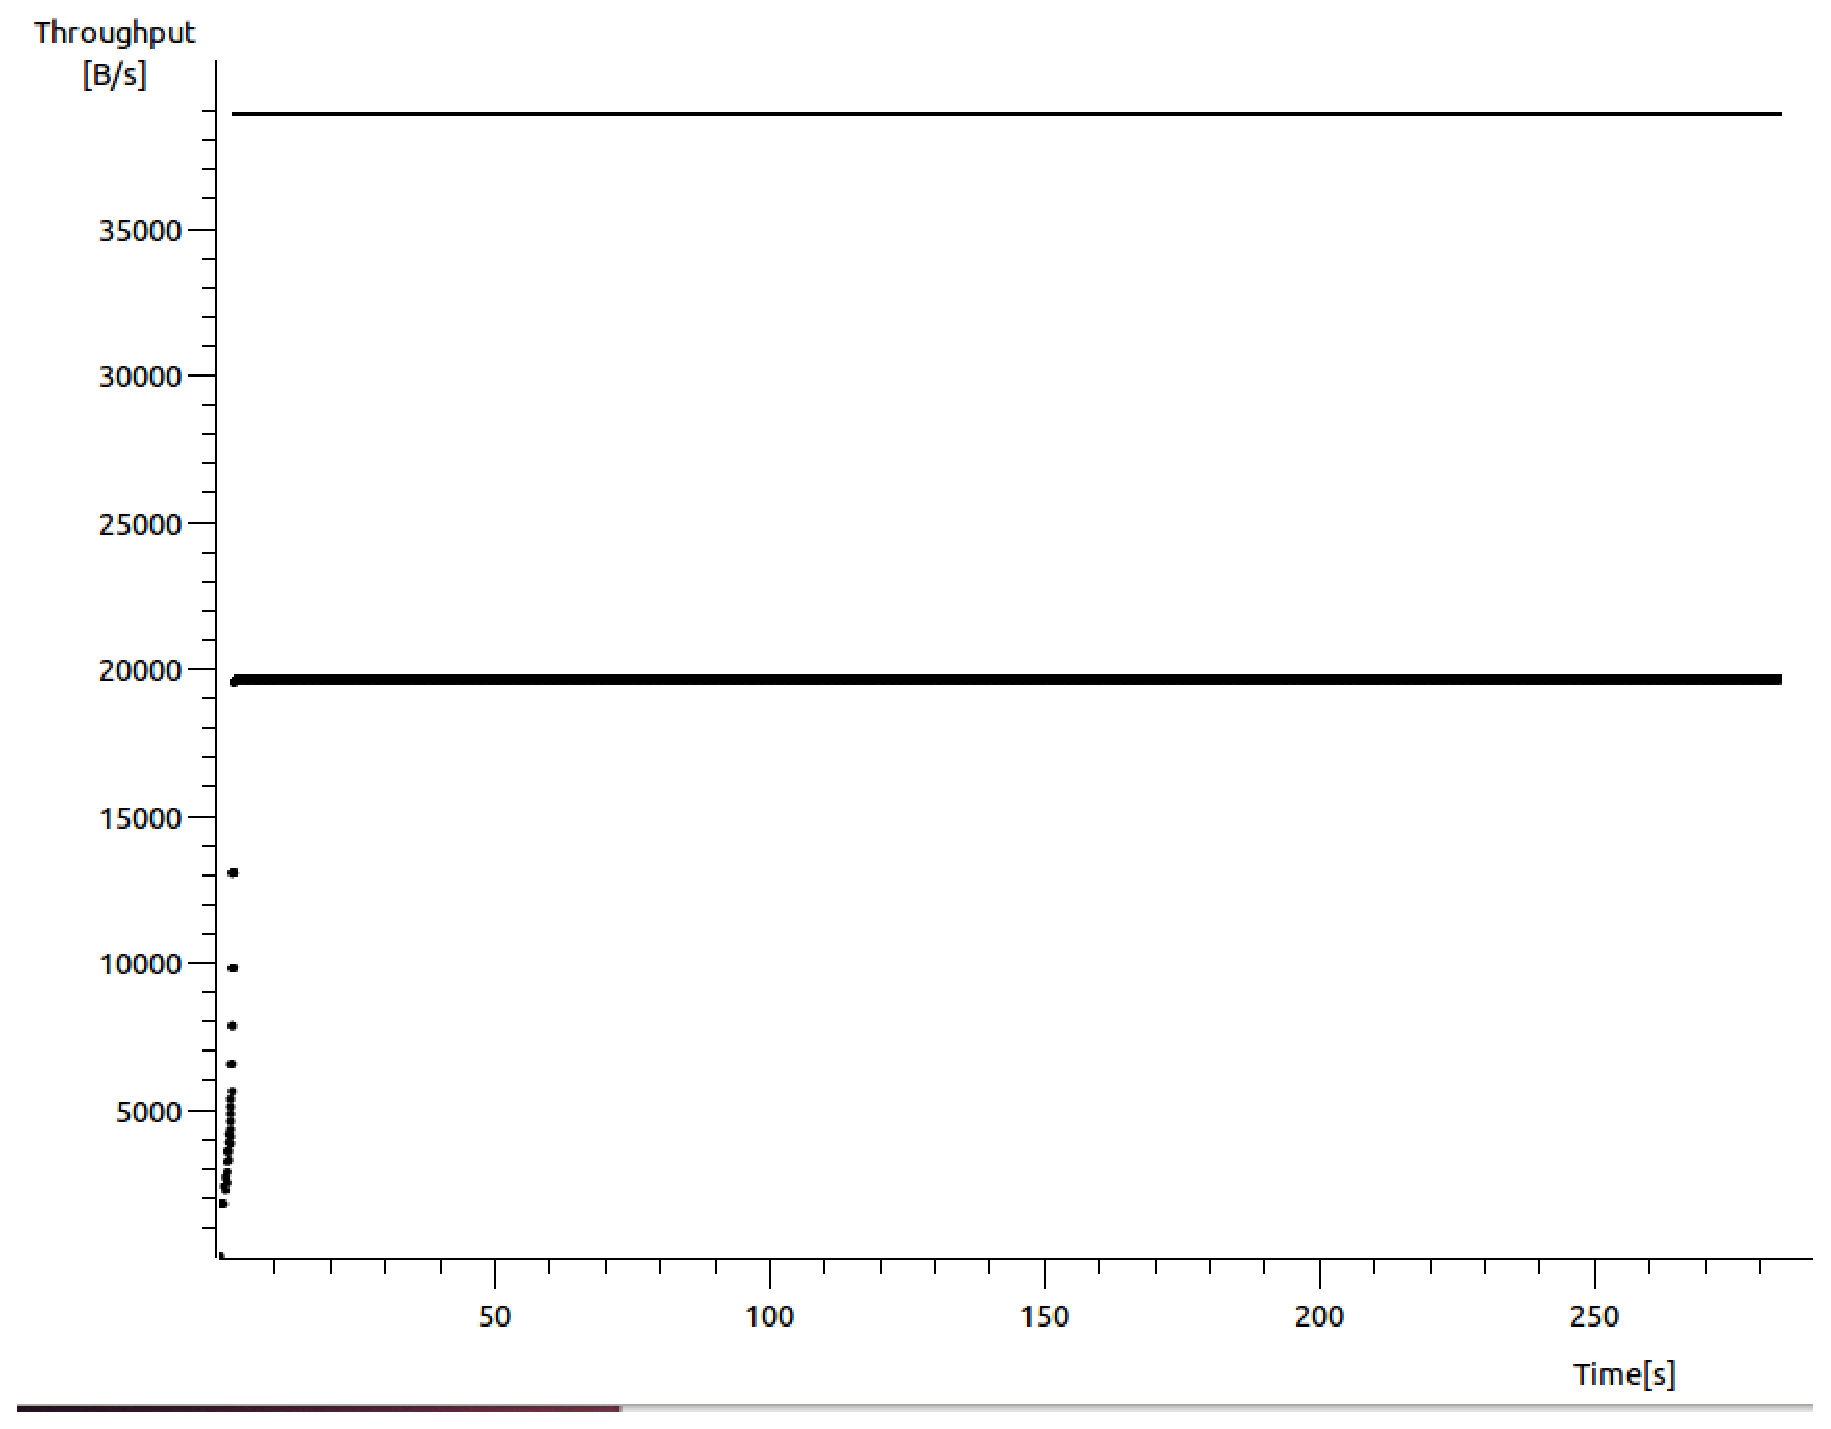
\includegraphics[width=\textwidth]{s7-1_th}
  \caption{Throughput}
 \end{subfigure}
 \begin{subfigure}[b]{0.2\textwidth}
  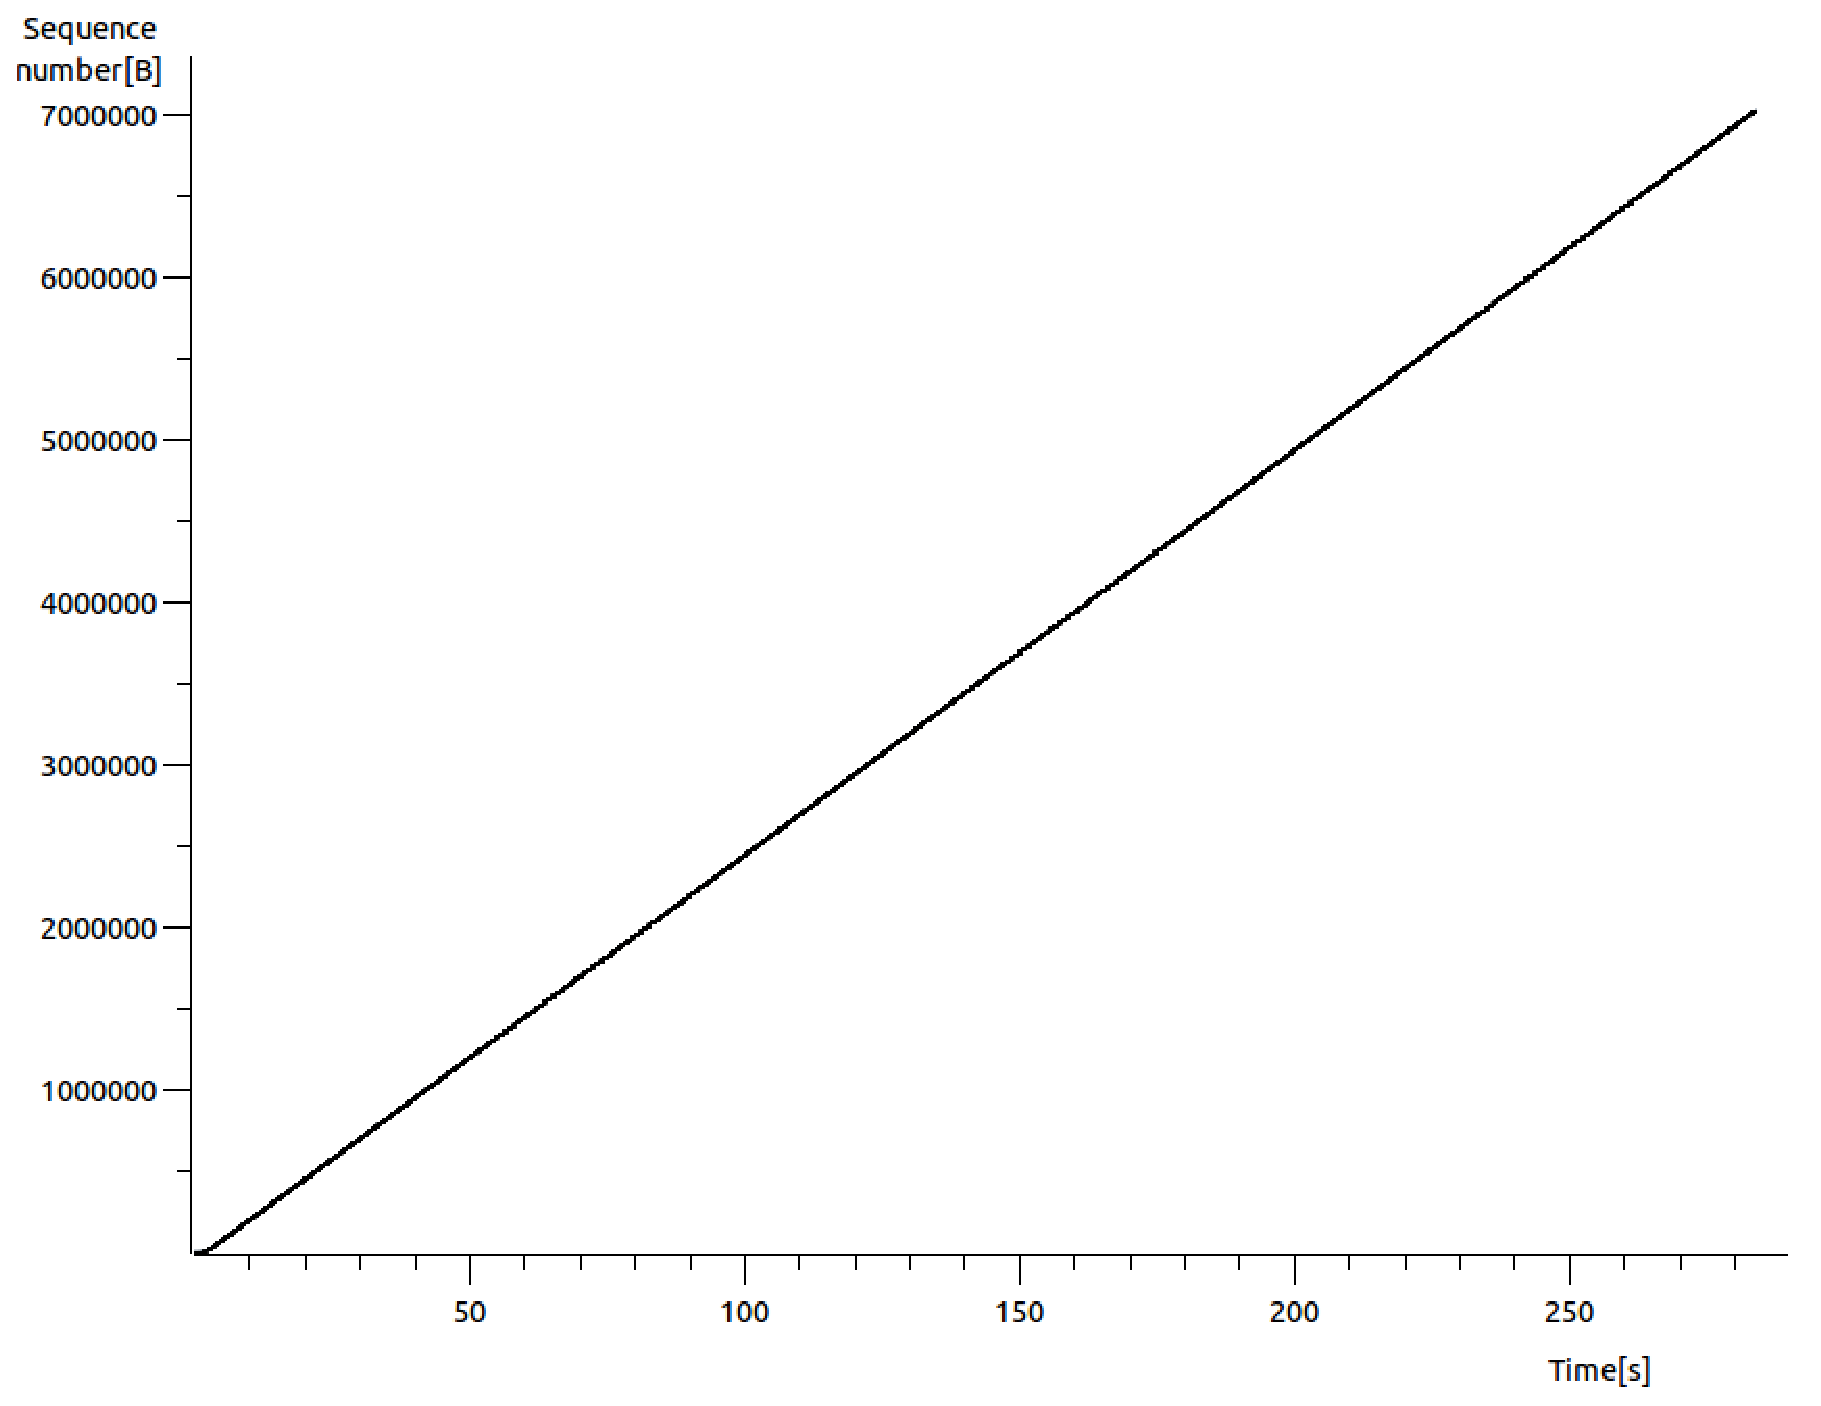
\includegraphics[width=\textwidth]{s7-1_seq}
  \caption{TCP sequence}
 \end{subfigure}
 \begin{subfigure}[b]{0.2\textwidth}
  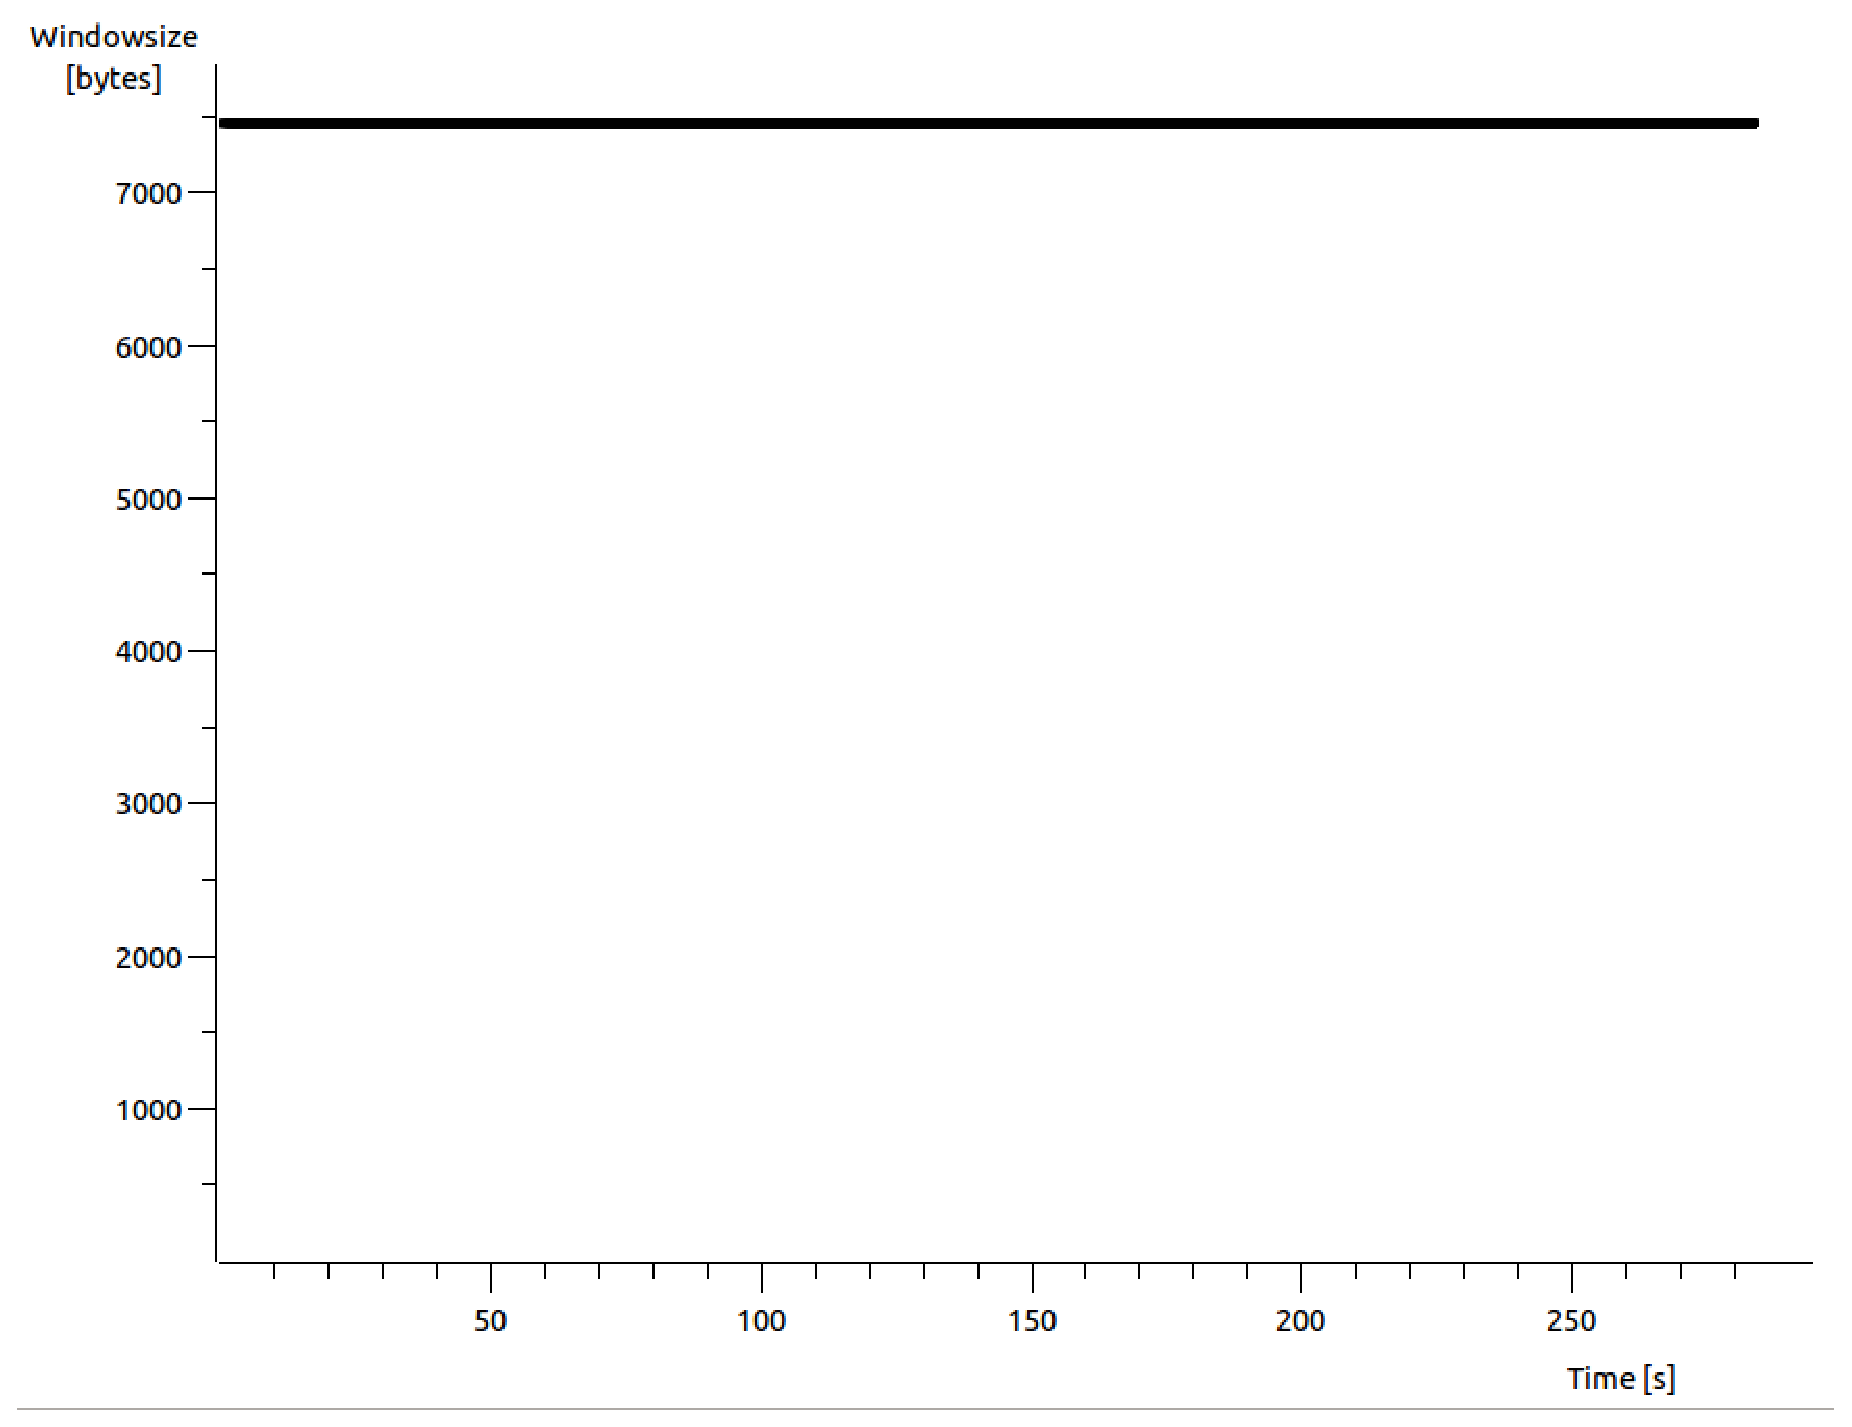
\includegraphics[width=\textwidth]{s7-1_wsize}
  \caption{Window size}
 \end{subfigure}
 \begin{subfigure}[b]{0.2\textwidth}
  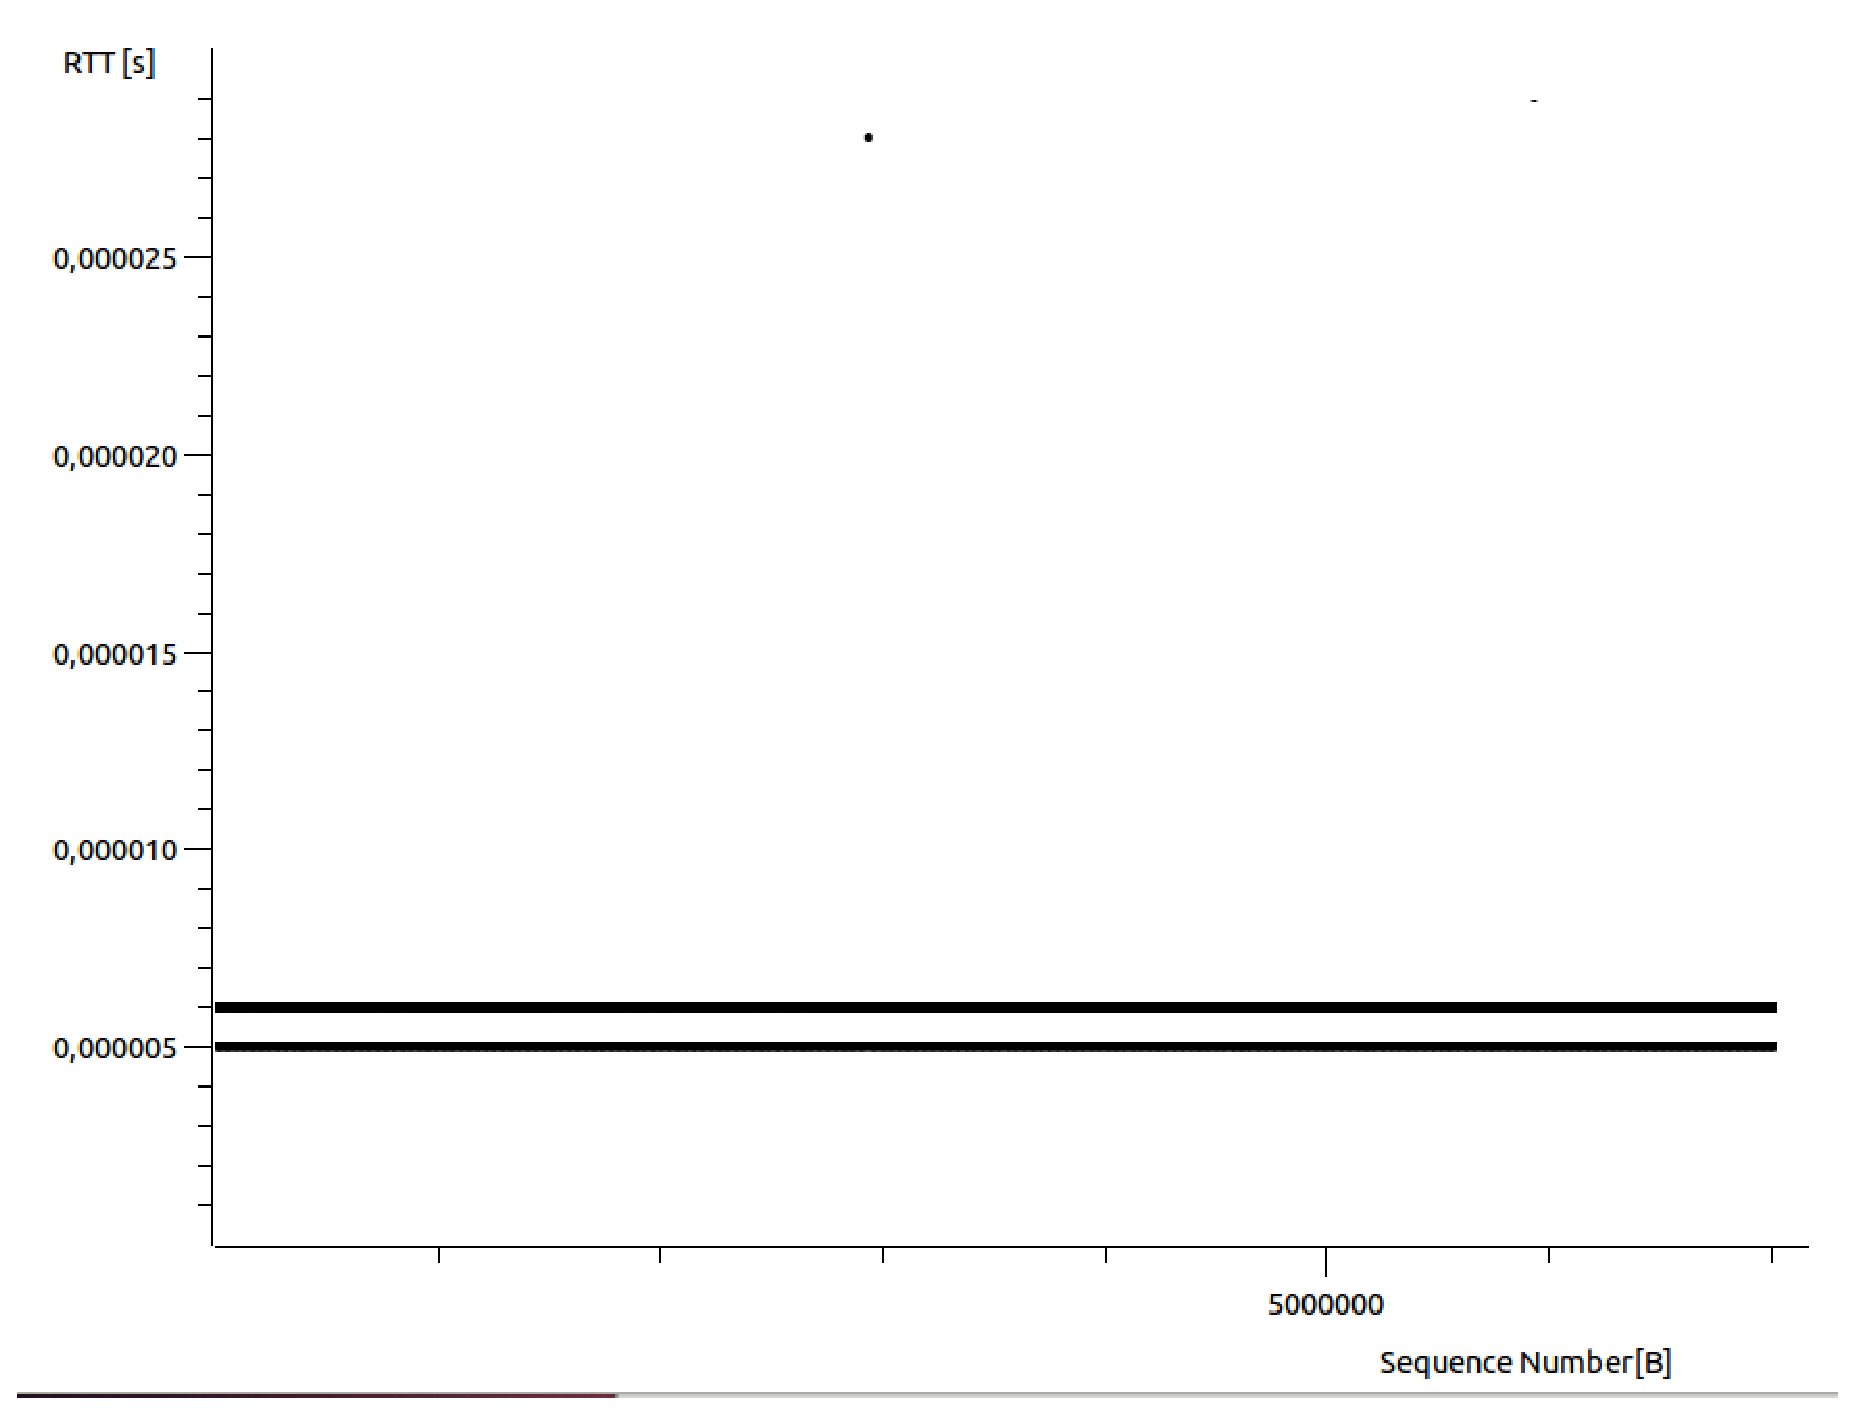
\includegraphics[width=\textwidth]{s7-1_rtt}
  \caption{RTT}
 \end{subfigure}
 \caption{Scene 7-1: TCP Vegas + 50 ms delay}
\end{figure}

\begin{figure}
 \centering
 \begin{subfigure}[b]{0.2\textwidth}
  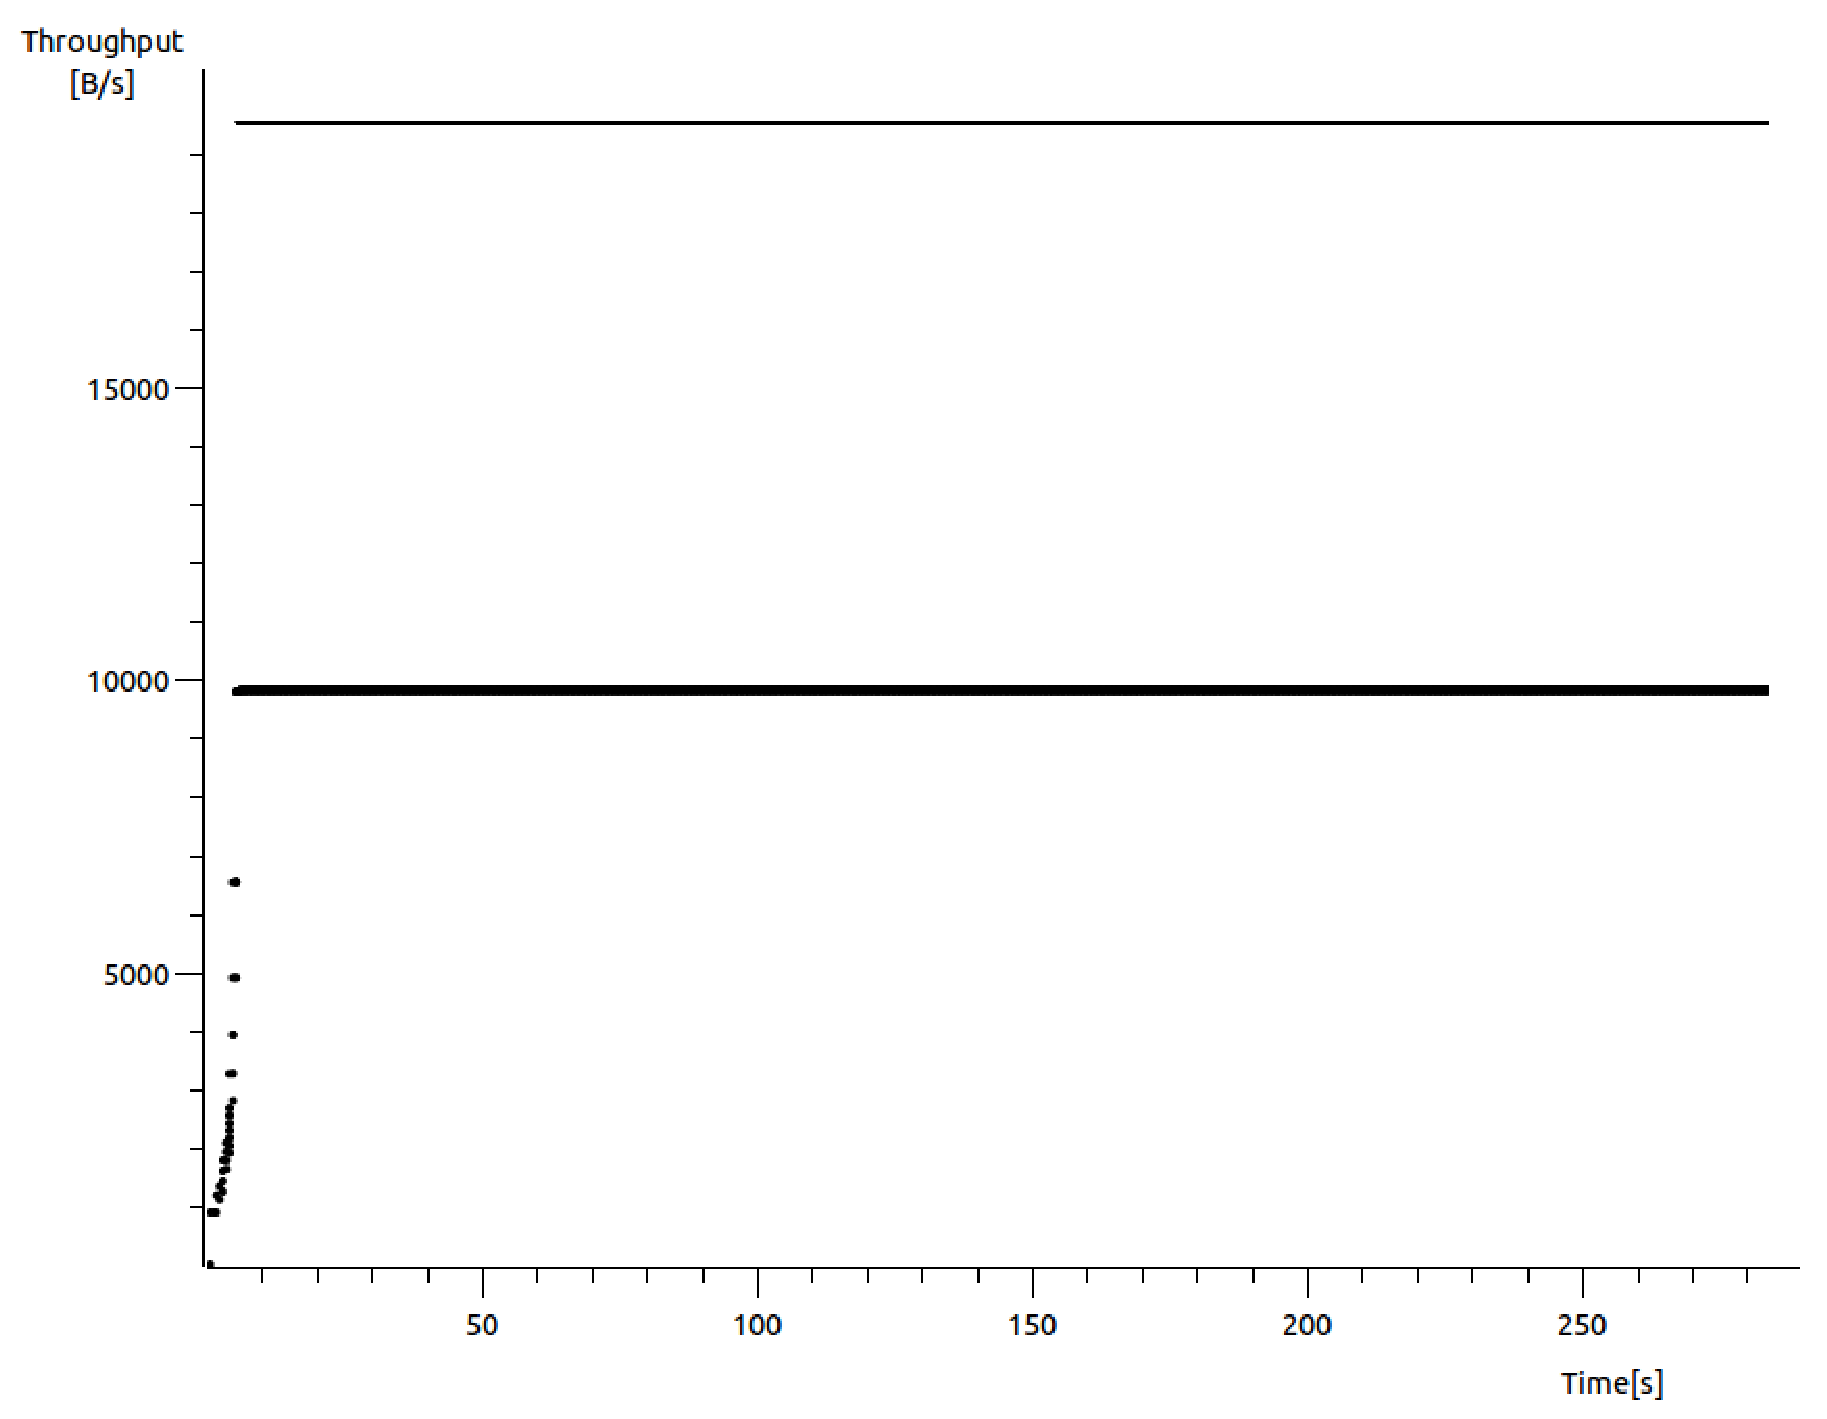
\includegraphics[width=\textwidth]{s7-2_th}
  \caption{Throughput}
 \end{subfigure}
 \begin{subfigure}[b]{0.2\textwidth}
  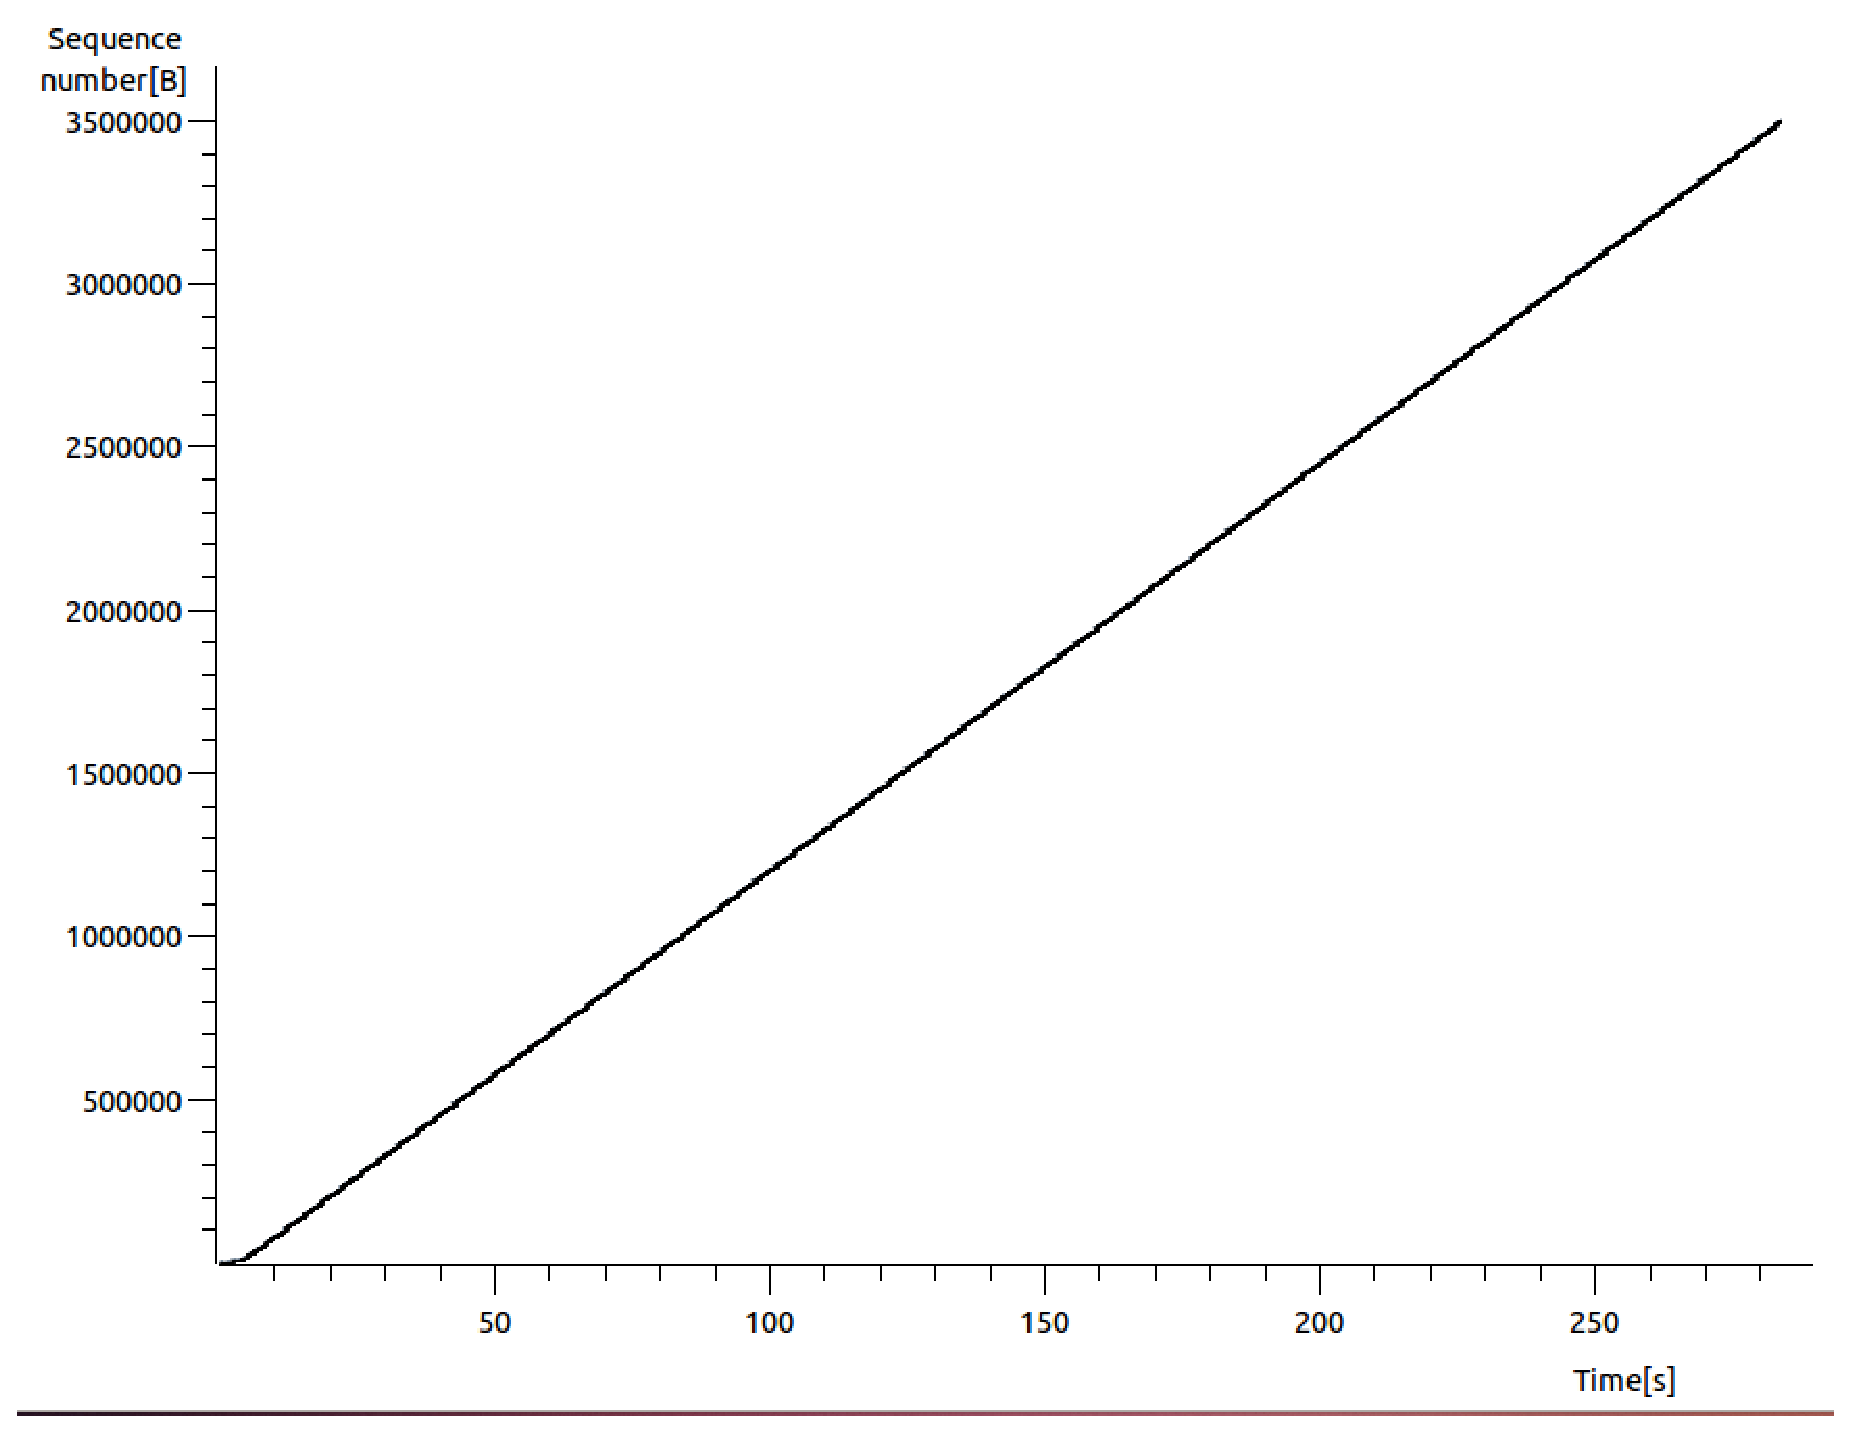
\includegraphics[width=\textwidth]{s7-2_seq}
  \caption{TCP sequence}
 \end{subfigure}
 \begin{subfigure}[b]{0.2\textwidth}
  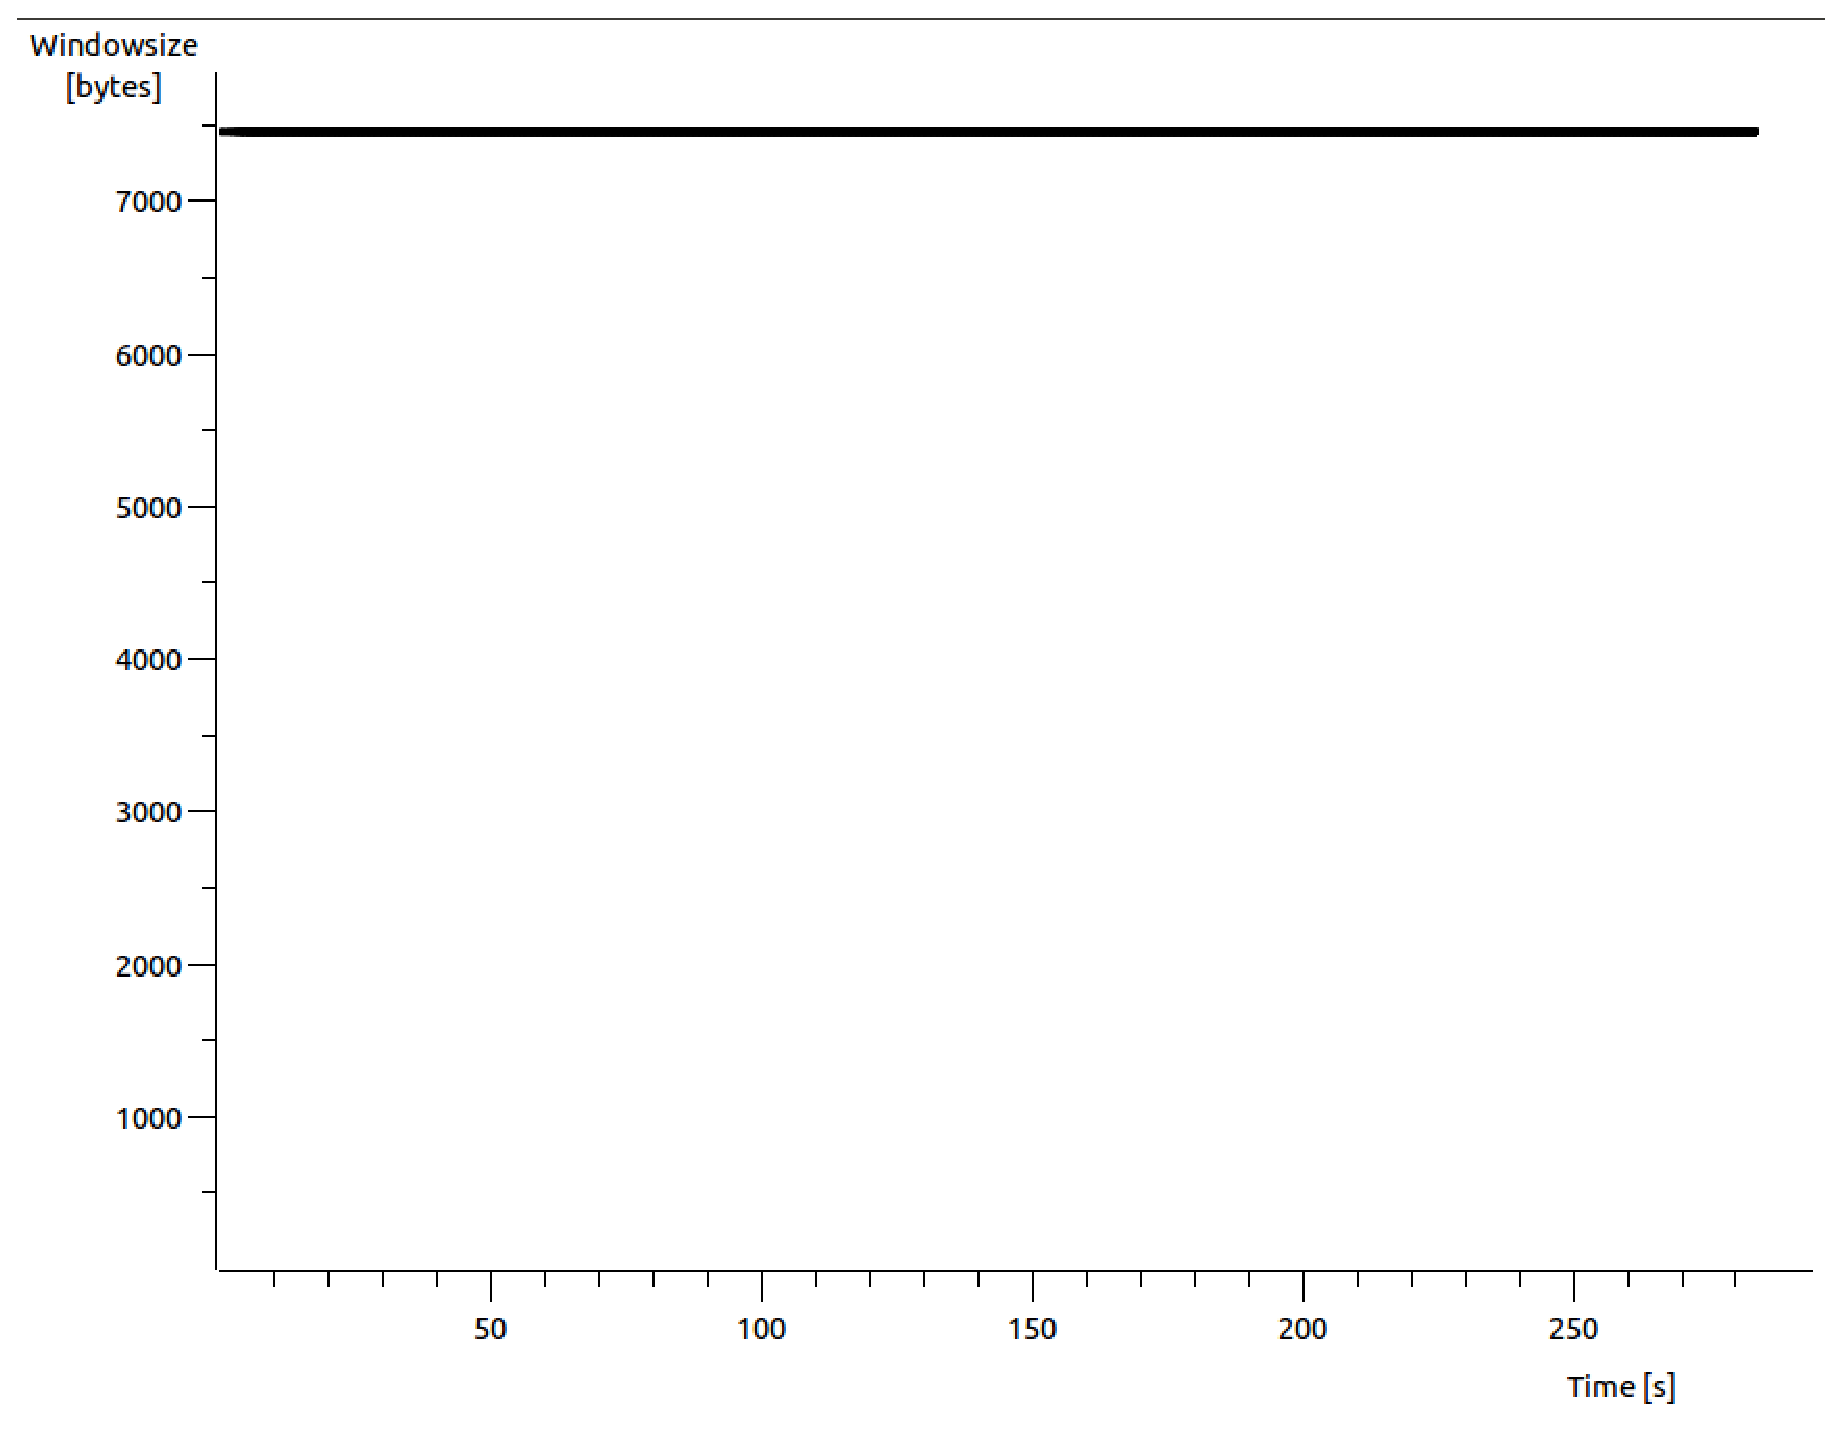
\includegraphics[width=\textwidth]{s7-2_wsize}
  \caption{Window size}
 \end{subfigure}
 \begin{subfigure}[b]{0.2\textwidth}
  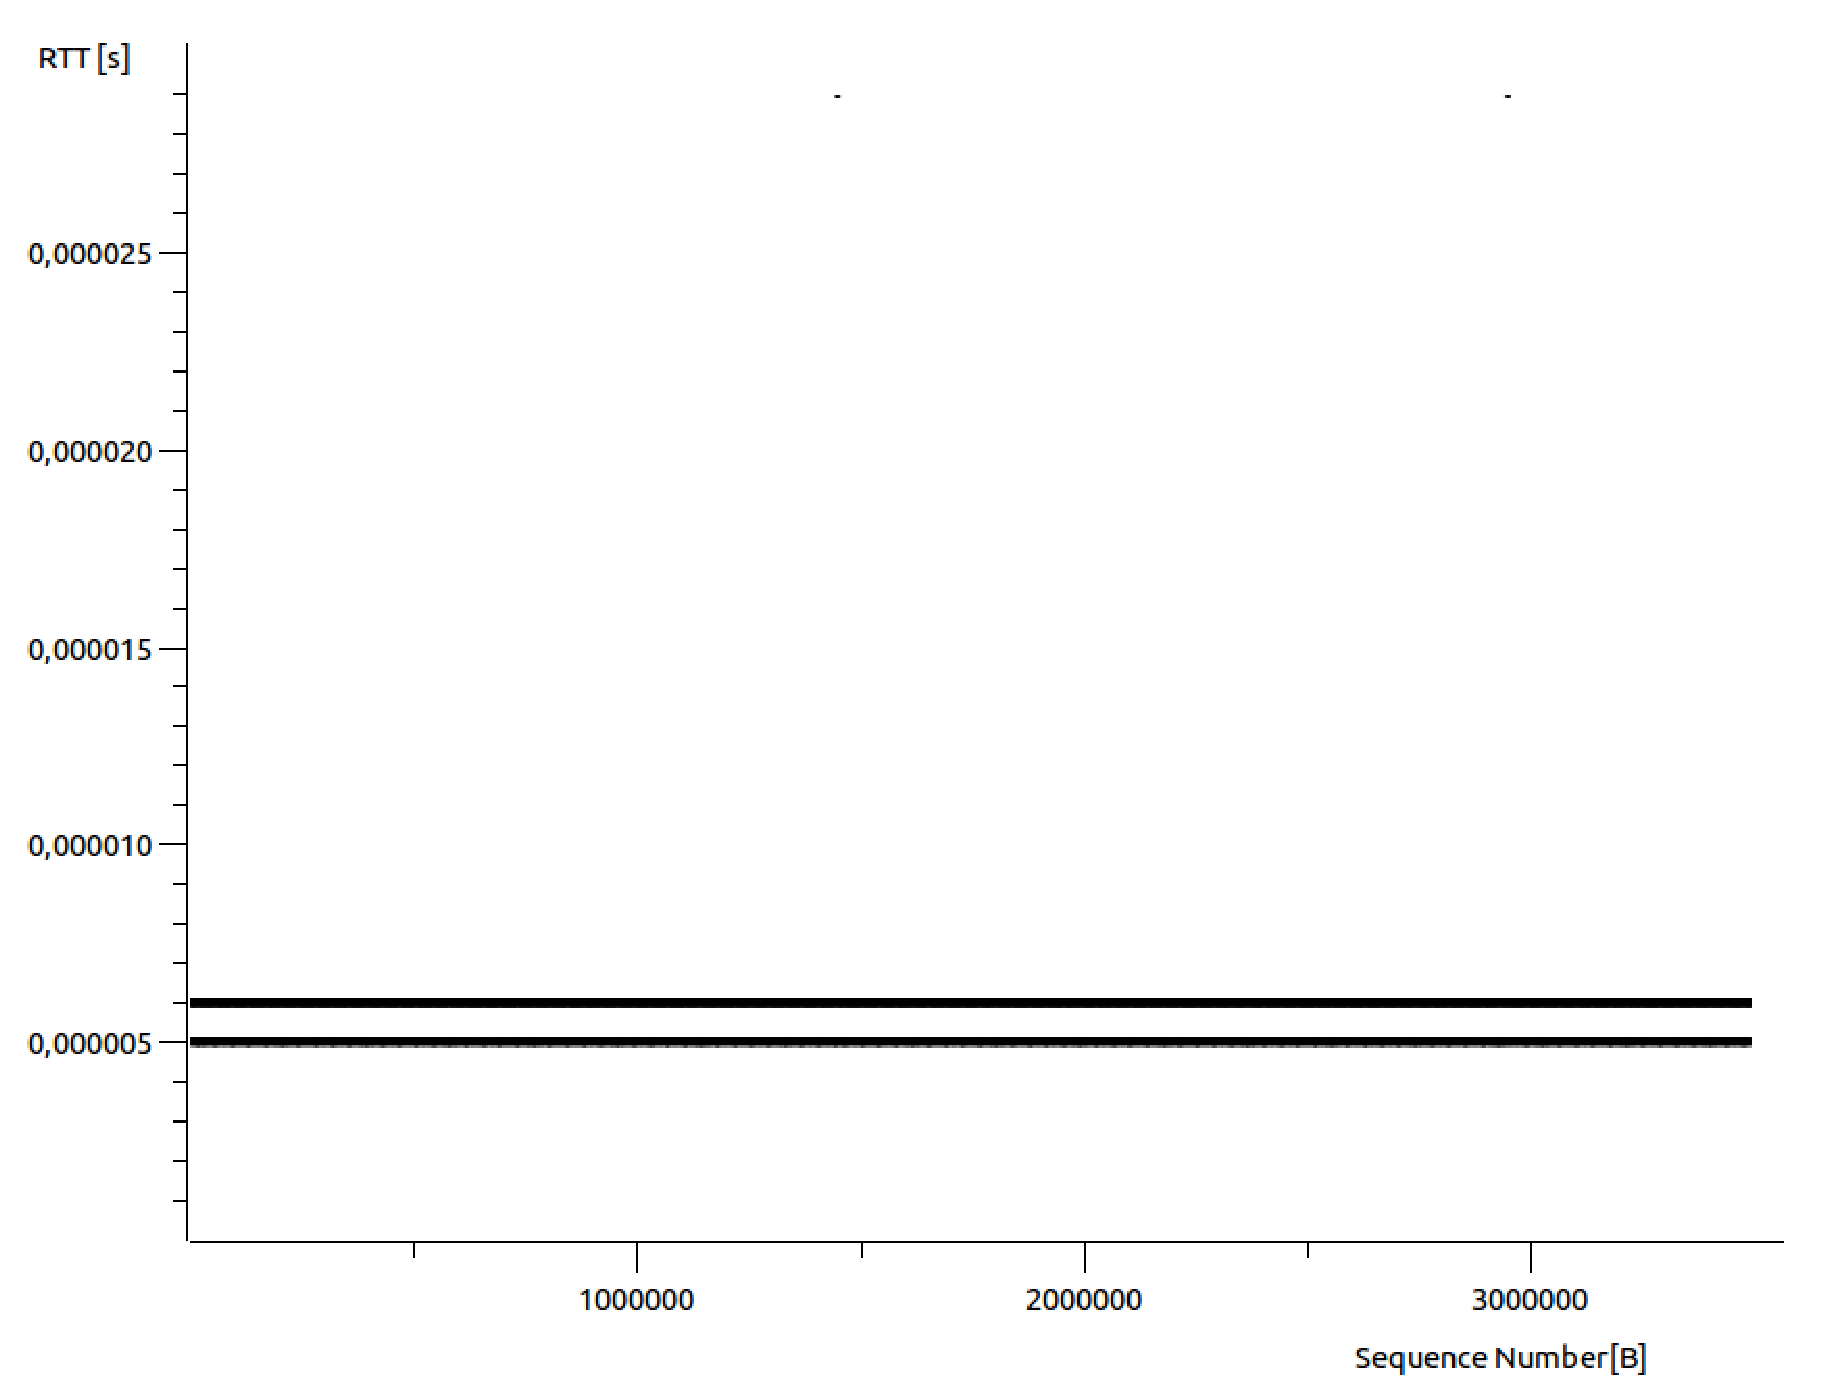
\includegraphics[width=\textwidth]{s7-2_rtt}
  \caption{RTT}
 \end{subfigure}
 \caption{Scene 7-2: TCP Vegas + 200 ms delay}
\end{figure}

\begin{figure}
 \centering
 \begin{subfigure}[b]{0.2\textwidth}
  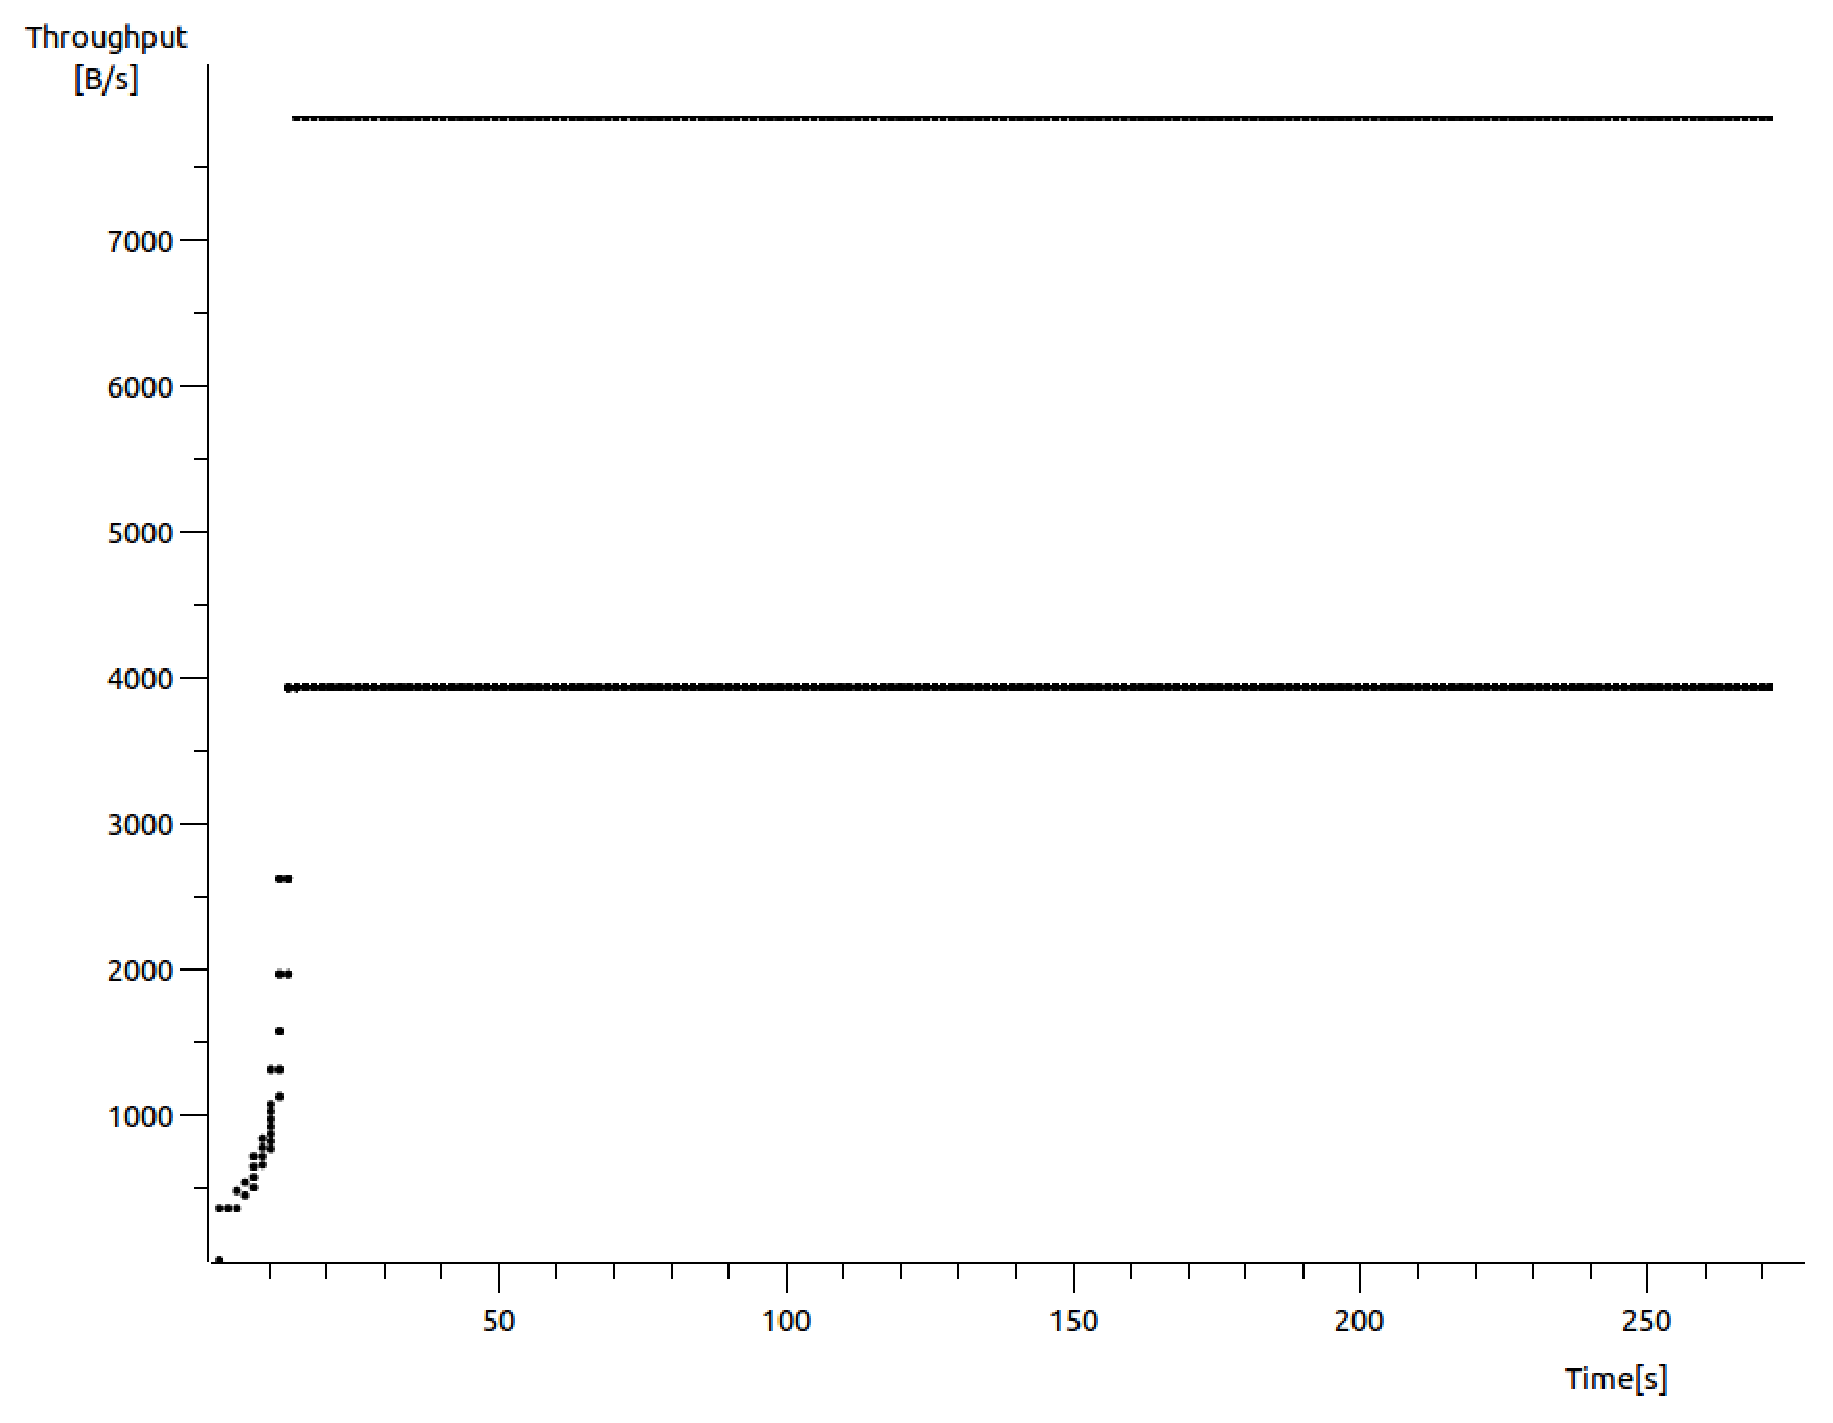
\includegraphics[width=\textwidth]{s7-3_th}
  \caption{Throughput}
 \end{subfigure}
 \begin{subfigure}[b]{0.2\textwidth}
  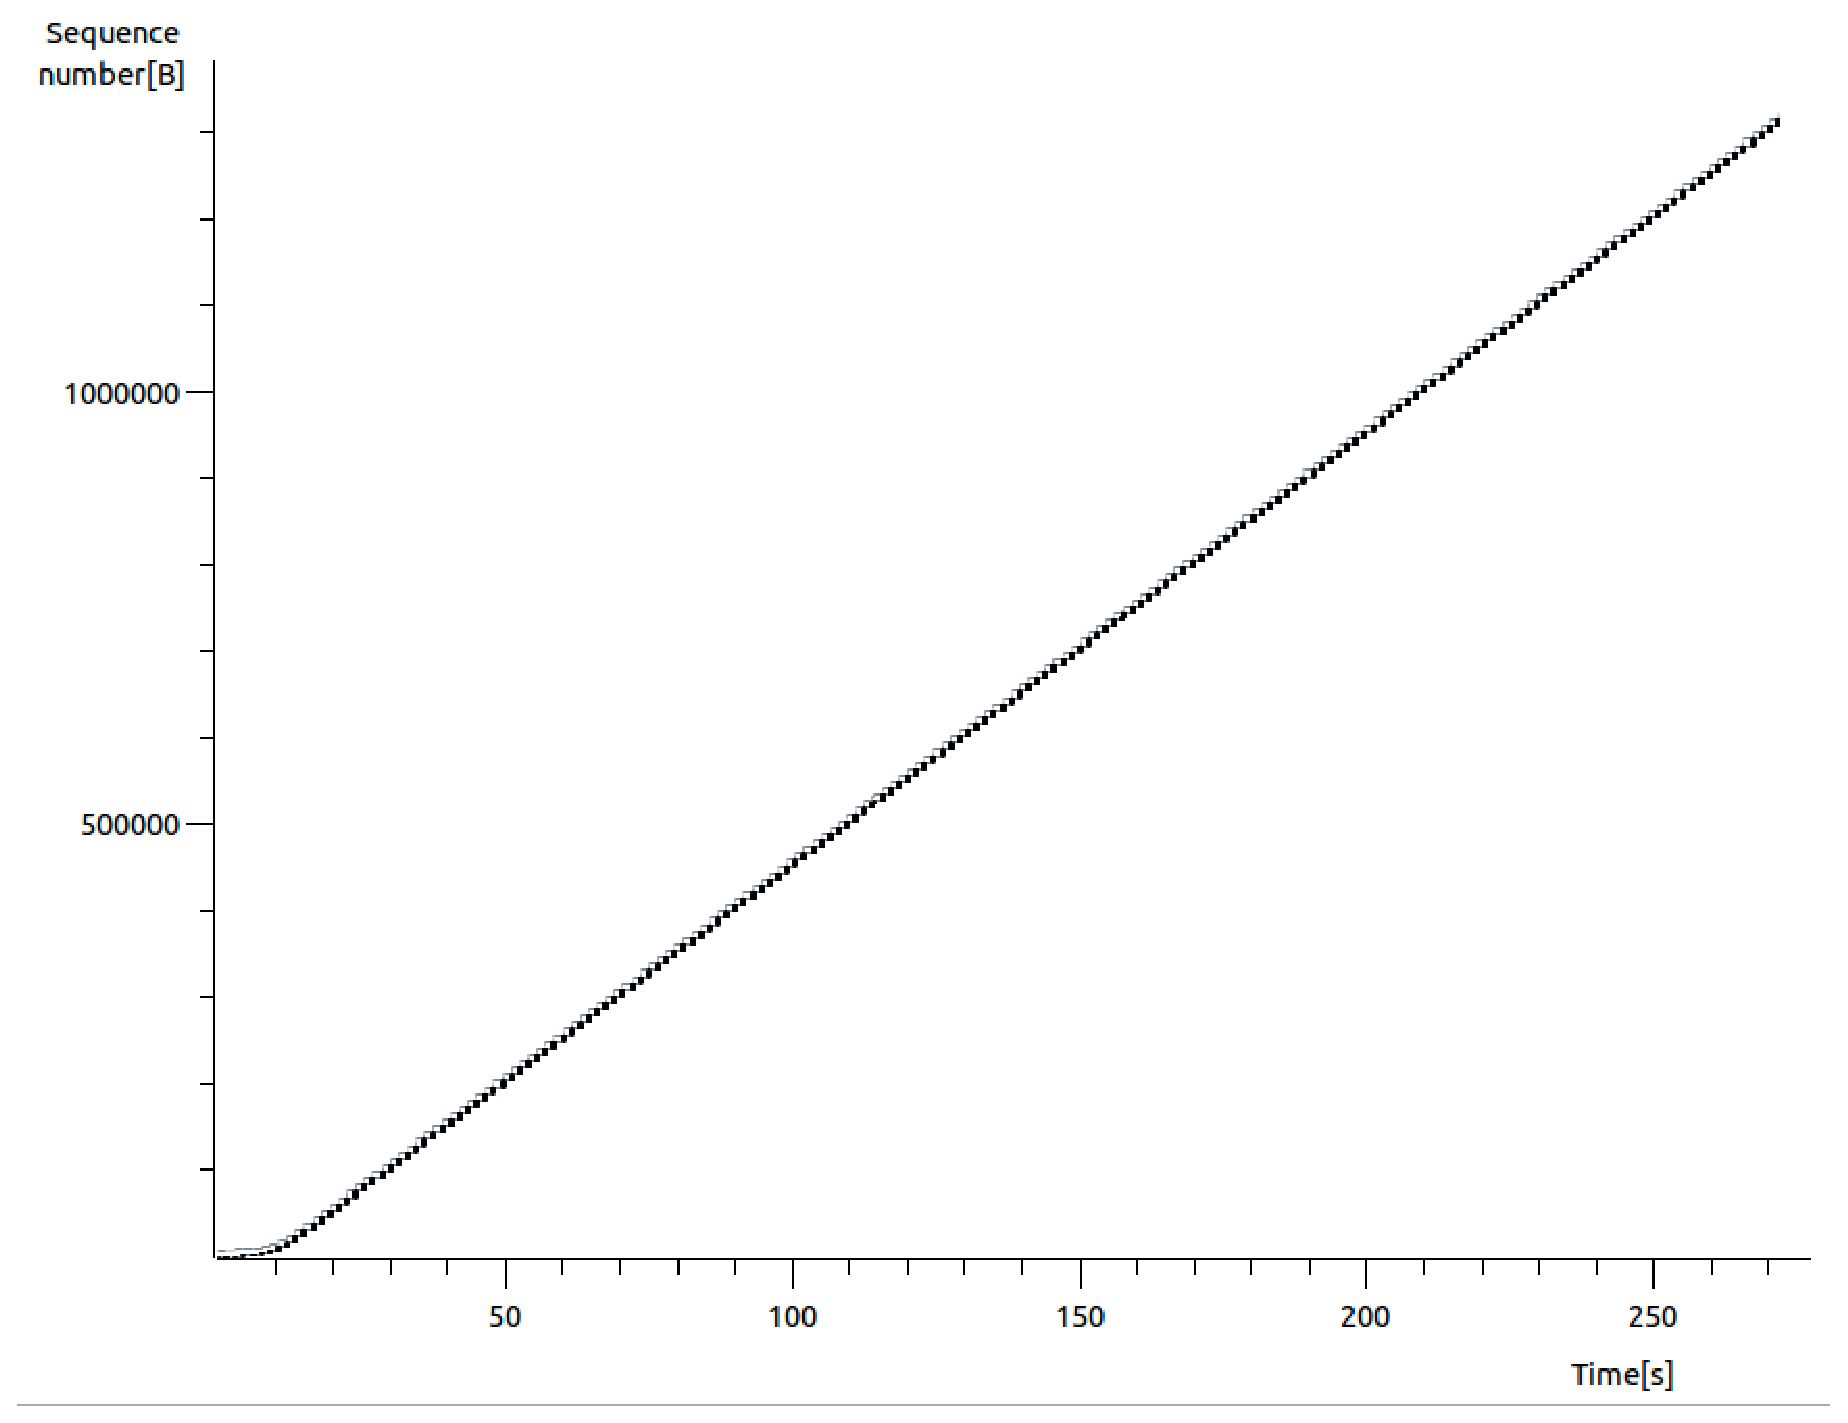
\includegraphics[width=\textwidth]{s7-3_seq}
  \caption{TCP sequence}
 \end{subfigure}
 \begin{subfigure}[b]{0.2\textwidth}
  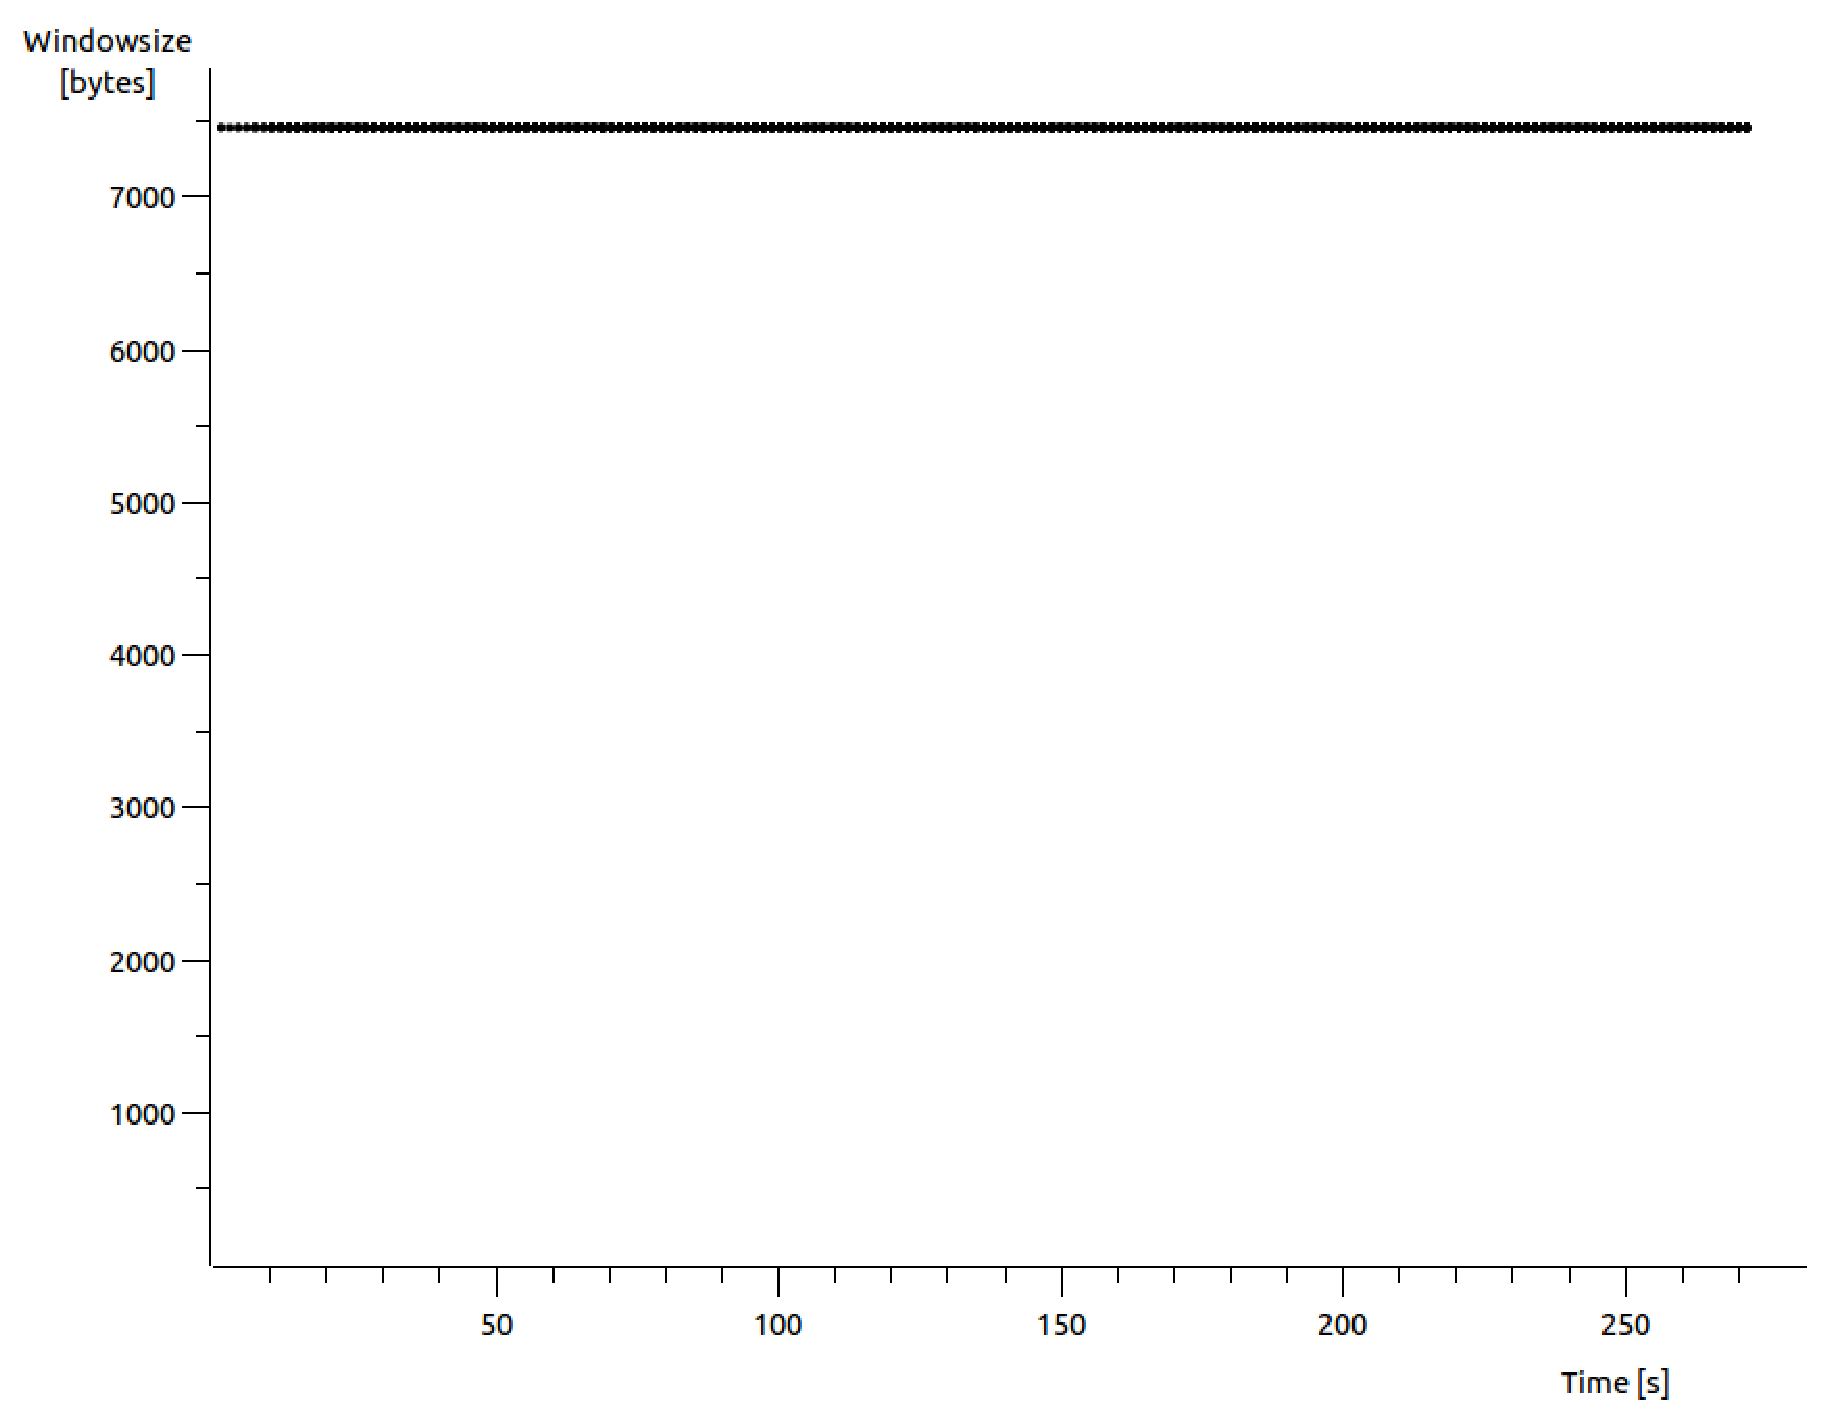
\includegraphics[width=\textwidth]{s7-3_wsize}
  \caption{Window size}
 \end{subfigure}
 \begin{subfigure}[b]{0.2\textwidth}
  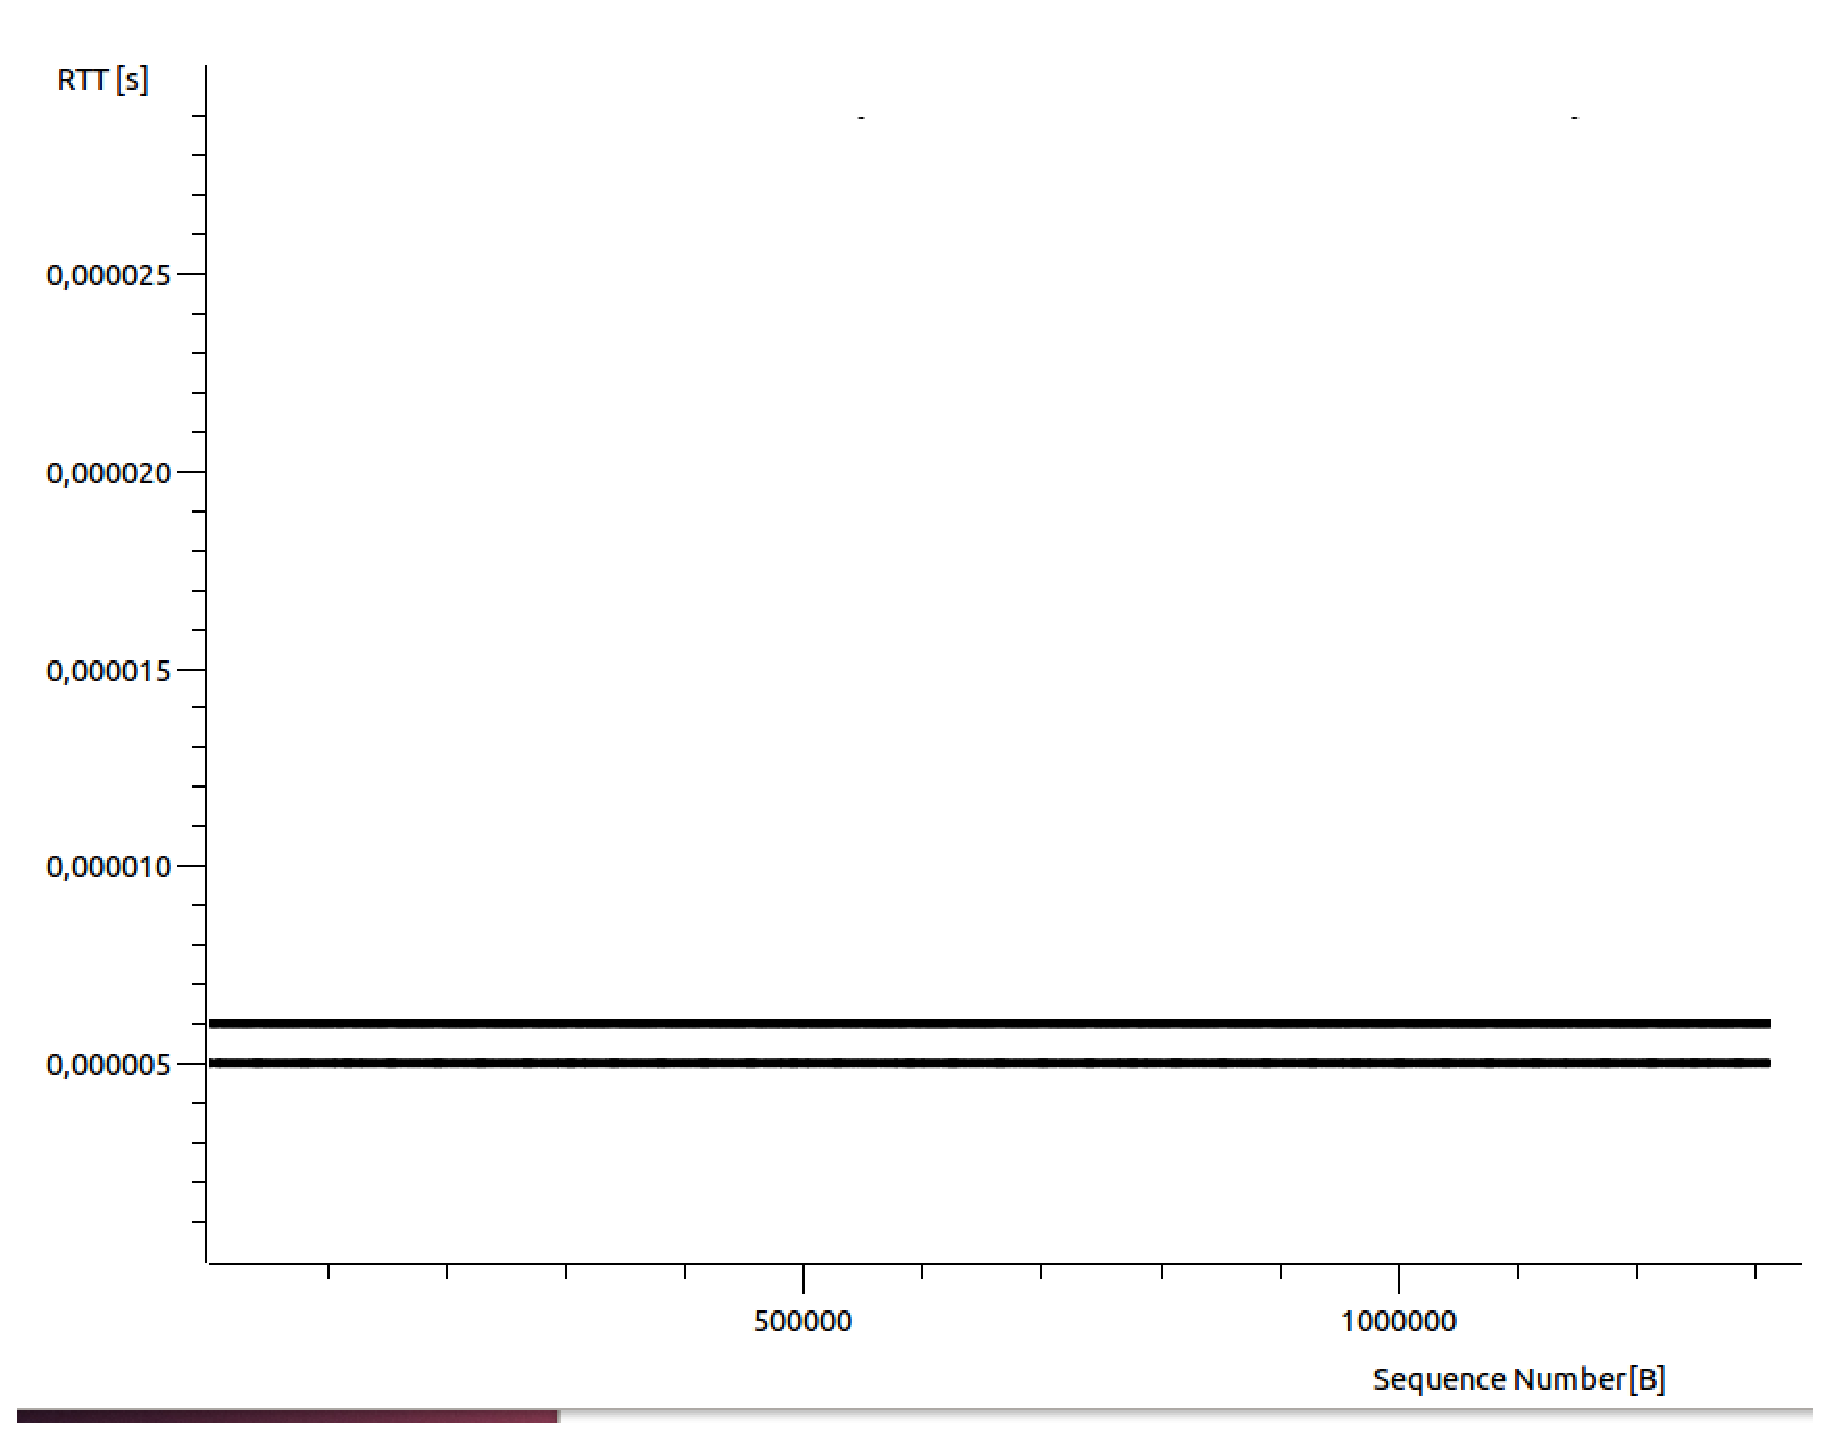
\includegraphics[width=\textwidth]{s7-3_rtt}
  \caption{RTT}
 \end{subfigure}
 \caption{Scene 7-3: TCP Vegas + 250 delay}
\end{figure}

\clearpage
% == packet error


\begin{figure}
 \centering
 \begin{subfigure}[b]{0.2\textwidth}
  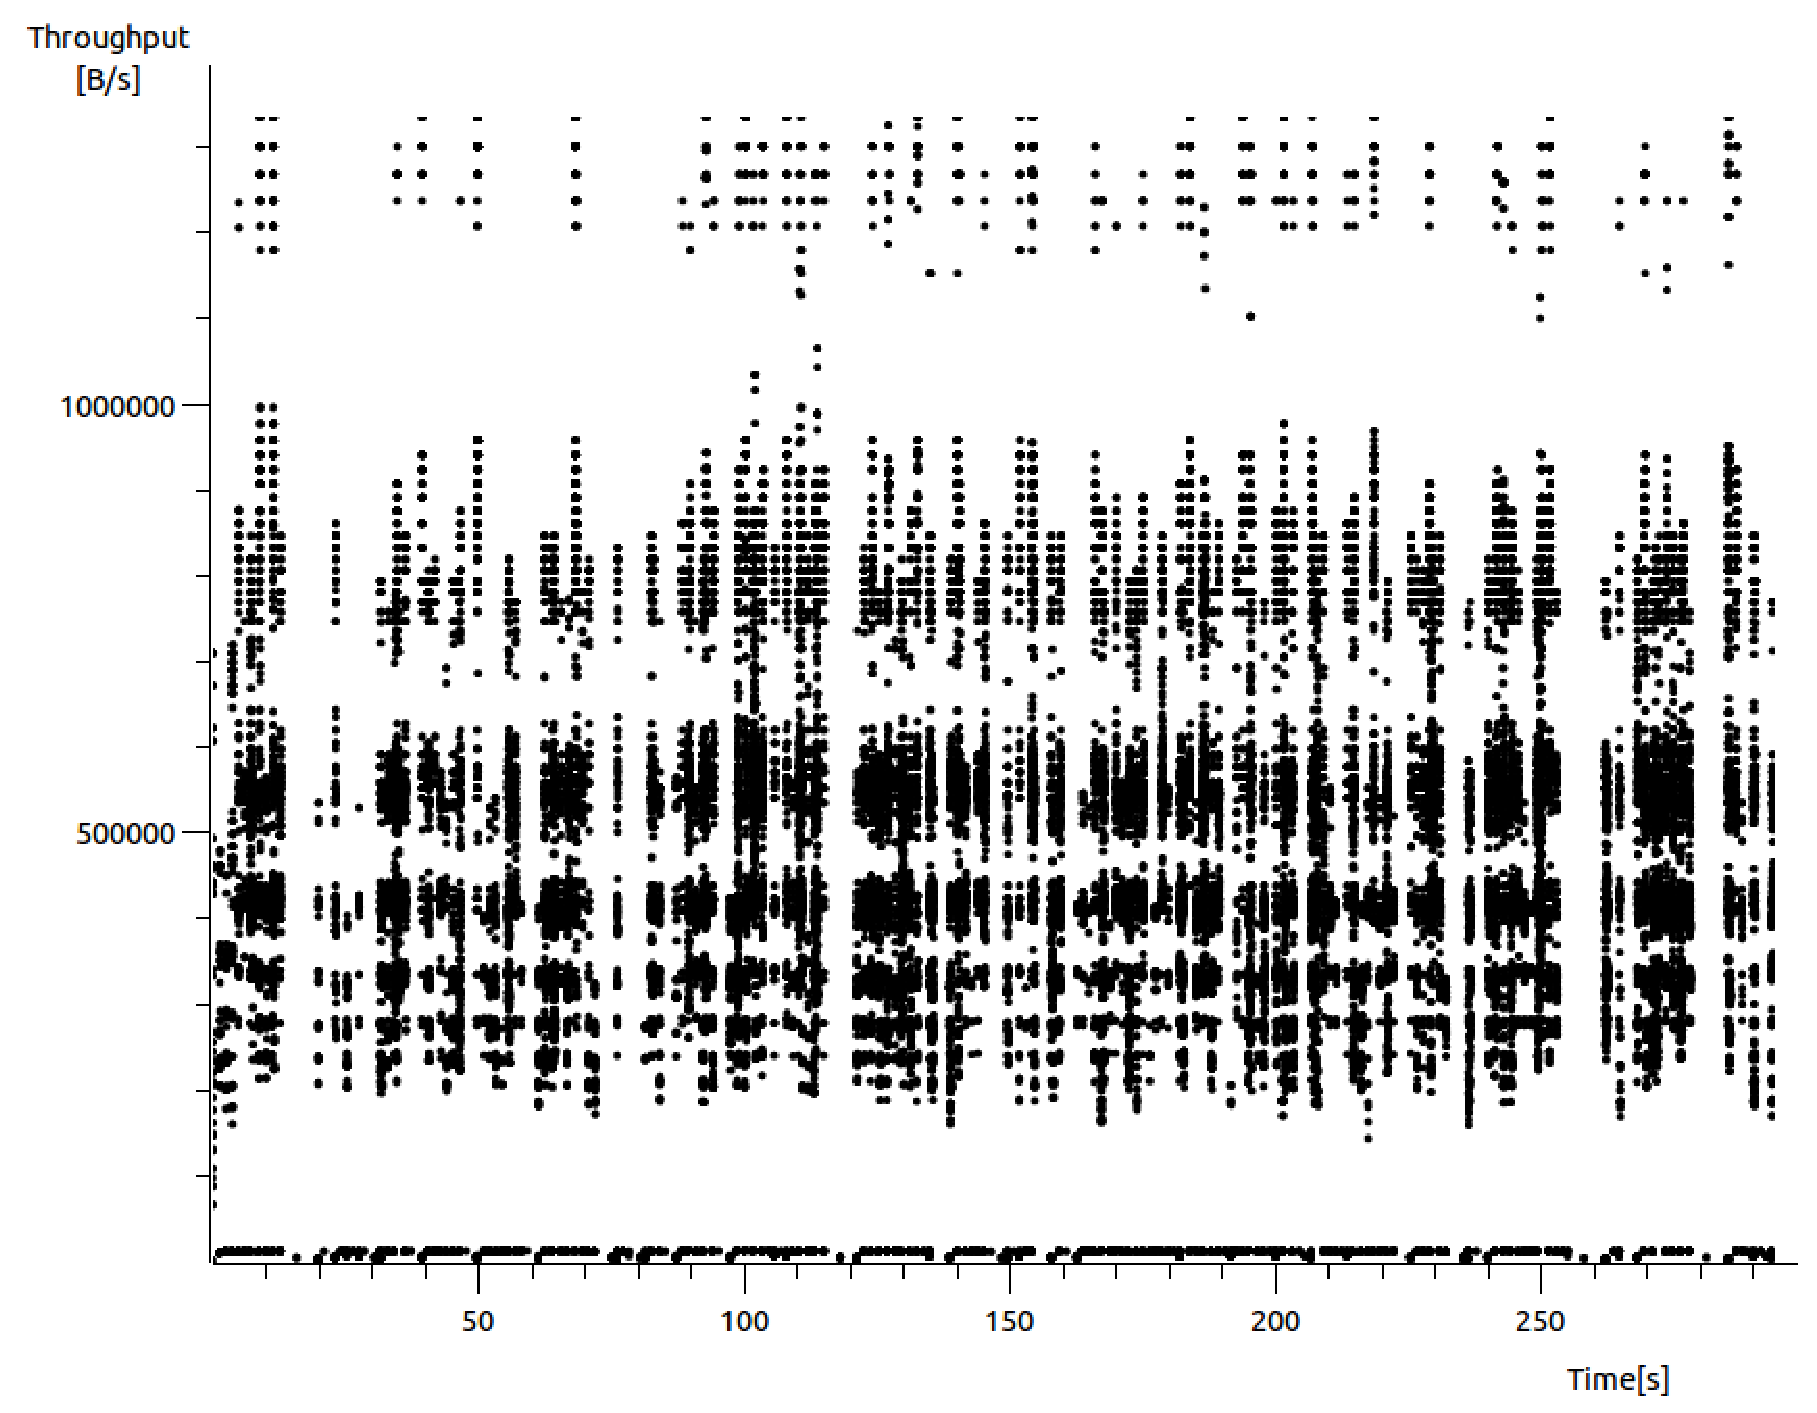
\includegraphics[width=\textwidth]{s2-0_thru}
  \caption{Throughput}
 \end{subfigure}
 \begin{subfigure}[b]{0.2\textwidth}
  \includegraphics[width=\textwidth]{s2-0_seq}
  \caption{TCP sequence}
 \end{subfigure}
 \begin{subfigure}[b]{0.2\textwidth}
  \includegraphics[width=\textwidth]{s2-0_wnd}
  \caption{Window size}
 \end{subfigure}
 \begin{subfigure}[b]{0.2\textwidth}
  \includegraphics[width=\textwidth]{s2-0_rtt}
  \caption{RTT}
 \end{subfigure}
 \caption{Scene 2-0: TCP Reno + 1\% error}
\end{figure}

\begin{figure}
 \centering
 \begin{subfigure}[b]{0.2\textwidth}
  \includegraphics[width=\textwidth]{s2-1_thru}
  \caption{Throughput}
 \end{subfigure}
 \begin{subfigure}[b]{0.2\textwidth}
  \includegraphics[width=\textwidth]{s2-1_seq}
  \caption{TCP sequence}
 \end{subfigure}
 \begin{subfigure}[b]{0.2\textwidth}
  \includegraphics[width=\textwidth]{s2-1_wnd}
  \caption{Window size}
 \end{subfigure}
 \begin{subfigure}[b]{0.2\textwidth}
  \includegraphics[width=\textwidth]{s2-1_rtt}
  \caption{RTT}
 \end{subfigure}
 \caption{Scene 2-1: TCP Reno + 5\% error}
\end{figure}

\begin{figure}
 \centering
 \begin{subfigure}[b]{0.2\textwidth}
  \includegraphics[width=\textwidth]{s2-2_thru}
  \caption{Throughput}
 \end{subfigure}
 \begin{subfigure}[b]{0.2\textwidth}
  \includegraphics[width=\textwidth]{s2-2_seq}
  \caption{TCP sequence}
 \end{subfigure}
 \begin{subfigure}[b]{0.2\textwidth}
  \includegraphics[width=\textwidth]{s2-2_wnd}
  \caption{Window size}
 \end{subfigure}
 \begin{subfigure}[b]{0.2\textwidth}
  \includegraphics[width=\textwidth]{s2-2_rtt}
  \caption{RTT}
 \end{subfigure}
 \caption{Scene 2-2: TCP Reno + 10\% error}
\end{figure}

\begin{figure}
 \centering
 \begin{subfigure}[b]{0.2\textwidth}
  \includegraphics[width=\textwidth]{s2-3_thru}
  \caption{Throughput}
 \end{subfigure}
 \begin{subfigure}[b]{0.2\textwidth}
  \includegraphics[width=\textwidth]{s2-3_seq}
  \caption{TCP sequence}
 \end{subfigure}
 \begin{subfigure}[b]{0.2\textwidth}
  \includegraphics[width=\textwidth]{s2-3_wnd}
  \caption{Window size}
 \end{subfigure}
 \begin{subfigure}[b]{0.2\textwidth}
  \includegraphics[width=\textwidth]{s2-3_rtt}
  \caption{RTT}
 \end{subfigure}
 \caption{Scene 2-3: TCP Reno + 20\% error}
\end{figure}


\begin{figure}
 \centering
 \begin{subfigure}[b]{0.2\textwidth}
  \includegraphics[width=\textwidth]{s5-0_th}
  \caption{Throughput}
 \end{subfigure}
 \begin{subfigure}[b]{0.2\textwidth}
  \includegraphics[width=\textwidth]{s5-0_seq}
  \caption{TCP sequence}
 \end{subfigure}
 \begin{subfigure}[b]{0.2\textwidth}
  \includegraphics[width=\textwidth]{s5-0_wsize}
  \caption{Window size}
 \end{subfigure}
 \begin{subfigure}[b]{0.2\textwidth}
  \includegraphics[width=\textwidth]{s5-0_rtt}
  \caption{RTT}
 \end{subfigure}
 \caption{Scene 5-0: TCP New Reno + 1\% error}
\end{figure}

\begin{figure}
 \centering
 \begin{subfigure}[b]{0.2\textwidth}
  \includegraphics[width=\textwidth]{s5-1_th}
  \caption{Throughput}
 \end{subfigure}
 \begin{subfigure}[b]{0.2\textwidth}
  \includegraphics[width=\textwidth]{s5-1_seq}
  \caption{TCP sequence}
 \end{subfigure}
 \begin{subfigure}[b]{0.2\textwidth}
  \includegraphics[width=\textwidth]{s5-1_wsize}
  \caption{Window size}
 \end{subfigure}
 \begin{subfigure}[b]{0.2\textwidth}
  \includegraphics[width=\textwidth]{s5-1_rtt}
  \caption{RTT}
 \end{subfigure}
 \caption{Scene 5-1: TCP New Reno + 5\% error}
\end{figure}

\begin{figure}
 \centering
 \begin{subfigure}[b]{0.2\textwidth}
  \includegraphics[width=\textwidth]{s5-2_th}
  \caption{Throughput}
 \end{subfigure}
 \begin{subfigure}[b]{0.2\textwidth}
  \includegraphics[width=\textwidth]{s5-2_seq}
  \caption{TCP sequence}
 \end{subfigure}
 \begin{subfigure}[b]{0.2\textwidth}
  \includegraphics[width=\textwidth]{s5-2_wsize}
  \caption{Window size}
 \end{subfigure}
 \begin{subfigure}[b]{0.2\textwidth}
  \includegraphics[width=\textwidth]{s5-2_rtt}
  \caption{RTT}
 \end{subfigure}
 \caption{Scene 5-2: TCP New Reno + 10\% error}
\end{figure}

\begin{figure}
 \centering
 \begin{subfigure}[b]{0.2\textwidth}
  \includegraphics[width=\textwidth]{s5-3_th}
  \caption{Throughput}
 \end{subfigure}
 \begin{subfigure}[b]{0.2\textwidth}
  \includegraphics[width=\textwidth]{s5-3_seq}
  \caption{TCP sequence}
 \end{subfigure}
 \begin{subfigure}[b]{0.2\textwidth}
  \includegraphics[width=\textwidth]{s5-3_wsize}
  \caption{Window size}
 \end{subfigure}
 \begin{subfigure}[b]{0.2\textwidth}
  \includegraphics[width=\textwidth]{s5-3_rtt}
  \caption{RTT}
 \end{subfigure}
 \caption{Scene 5-3: TCP New Reno + 20\% error}
\end{figure}

\begin{figure}
 \centering
 \begin{subfigure}[b]{0.2\textwidth}
  \includegraphics[width=\textwidth]{s8-0_th}
  \caption{Throughput}
 \end{subfigure}
 \begin{subfigure}[b]{0.2\textwidth}
  \includegraphics[width=\textwidth]{s8-0_seq}
  \caption{TCP sequence}
 \end{subfigure}
 \begin{subfigure}[b]{0.2\textwidth}
  \includegraphics[width=\textwidth]{s8-0_wsize}
  \caption{Window size}
 \end{subfigure}
 \begin{subfigure}[b]{0.2\textwidth}
  \includegraphics[width=\textwidth]{s8-0_rtt}
  \caption{RTT}
 \end{subfigure}
 \caption{Scene 8-0: TCP Vegas + 1\% error}
\end{figure}

\begin{figure}
 \centering
 \begin{subfigure}[b]{0.2\textwidth}
  \includegraphics[width=\textwidth]{s8-1_th}
  \caption{Throughput}
 \end{subfigure}
 \begin{subfigure}[b]{0.2\textwidth}
  \includegraphics[width=\textwidth]{s8-1_seq}
  \caption{TCP sequence}
 \end{subfigure}
 \begin{subfigure}[b]{0.2\textwidth}
  \includegraphics[width=\textwidth]{s8-1_wsize}
  \caption{Window size}
 \end{subfigure}
 \begin{subfigure}[b]{0.2\textwidth}
  \includegraphics[width=\textwidth]{s8-1_rtt}
  \caption{RTT}
 \end{subfigure}
 \caption{Scene 8-1: TCP Vegas + 5\% error}
\end{figure}

\begin{figure}
 \centering
 \begin{subfigure}[b]{0.2\textwidth}
  \includegraphics[width=\textwidth]{s8-2_th}
  \caption{Throughput}
 \end{subfigure}
 \begin{subfigure}[b]{0.2\textwidth}
  \includegraphics[width=\textwidth]{s8-2_seq}
  \caption{TCP sequence}
 \end{subfigure}
 \begin{subfigure}[b]{0.2\textwidth}
  \includegraphics[width=\textwidth]{s8-2_wsize}
  \caption{Window size}
 \end{subfigure}
 \begin{subfigure}[b]{0.2\textwidth}
  \includegraphics[width=\textwidth]{s8-2_rtt}
  \caption{RTT}
 \end{subfigure}
 \caption{Scene 8-2: TCP Vegas + 10\% error}
\end{figure}

\begin{figure}
 \centering
 \begin{subfigure}[b]{0.2\textwidth}
  \includegraphics[width=\textwidth]{s8-3_th}
  \caption{Throughput}
 \end{subfigure}
 \begin{subfigure}[b]{0.2\textwidth}
  \includegraphics[width=\textwidth]{s8-3_seq}
  \caption{TCP sequence}
 \end{subfigure}
 \begin{subfigure}[b]{0.2\textwidth}
  \includegraphics[width=\textwidth]{s8-3_wsize}
  \caption{Window size}
 \end{subfigure}
 \begin{subfigure}[b]{0.2\textwidth}
  \includegraphics[width=\textwidth]{s8-3_rtt}
  \caption{RTT}
 \end{subfigure}
 \caption{Scene 8-3: TCP Vegas + 20\% error}
\end{figure}

% ==== routes
\clearpage

\begin{figure}
 \centering
 \begin{subfigure}[b]{0.2\textwidth}
  \includegraphics[width=\textwidth]{s3-0_thru}
  \caption{Throughput}
 \end{subfigure}
 \begin{subfigure}[b]{0.2\textwidth}
  \includegraphics[width=\textwidth]{s3-0_seq}
  \caption{TCP sequence}
 \end{subfigure}
 \begin{subfigure}[b]{0.2\textwidth}
  \includegraphics[width=\textwidth]{s3-0_wnd}
  \caption{Window size}
 \end{subfigure}
 \begin{subfigure}[b]{0.2\textwidth}
  \includegraphics[width=\textwidth]{s3-0_rtt}
  \caption{RTT}
 \end{subfigure}
 \caption{Scene 3: TCP Reno + Router failure}
\end{figure}

\begin{figure}
 \centering
 \begin{subfigure}[b]{0.2\textwidth}
  \includegraphics[width=\textwidth]{s6-0_th}
  \caption{Throughput}
 \end{subfigure}
 \begin{subfigure}[b]{0.2\textwidth}
  \includegraphics[width=\textwidth]{s6-0_seq}
  \caption{TCP sequence}
 \end{subfigure}
 \begin{subfigure}[b]{0.2\textwidth}
  \includegraphics[width=\textwidth]{s6-0_wsize}
  \caption{Window size}
 \end{subfigure}
 \begin{subfigure}[b]{0.2\textwidth}
  \includegraphics[width=\textwidth]{s6-0_rtt}
  \caption{RTT}
 \end{subfigure}
 \caption{Scene 6: TCP New Reno + Router failure}
\end{figure}

\begin{figure}
 \centering
 \begin{subfigure}[b]{0.2\textwidth}
  \includegraphics[width=\textwidth]{s9-0_th}
  \caption{Throughput}
 \end{subfigure}
 \begin{subfigure}[b]{0.2\textwidth}
  \includegraphics[width=\textwidth]{s9-0_seq}
  \caption{TCP sequence}
 \end{subfigure}
 \begin{subfigure}[b]{0.2\textwidth}
  \includegraphics[width=\textwidth]{s9-0_wsize}
  \caption{Window size}
 \end{subfigure}
 \begin{subfigure}[b]{0.2\textwidth}
  \includegraphics[width=\textwidth]{s9-0_rtt}
  \caption{RTT}
 \end{subfigure}
 \caption{Scene 9: TCP Vegas + Router failure}
\end{figure}


\section{Analysis}


\section{Conclusion}
Our implementation is available at: \url{https://github.com/zwuh/heat_ble/}.


\section*{Acknowledgement}
The authors would like to thank Vu Ba Tien Dung for his guidance throughout this project.



% trigger a \newpage just before the given reference
% number - used to balance the columns on the last page
% adjust value as needed - may need to be readjusted if
% the document is modified later
%\IEEEtriggeratref{8}
% The "triggered" command can be changed if desired:
%\IEEEtriggercmd{\enlargethispage{-5in}}

% references section
\nocite*{}
\bibliographystyle{../../sty/IEEEtran}
\bibliography{omnet}


\end{document}

